% Verification review document (generated by explaneat export verification-pack).
\documentclass[a4paper,11pt]{article}
\usepackage[margin=2.2cm]{geometry}
\usepackage{amsmath}
\usepackage{amssymb}
\usepackage{booktabs}
\usepackage{tabularx}
\usepackage{graphicx}
\usepackage[table,usenames,dvipsnames]{xcolor}
\usepackage{tikz}
\usetikzlibrary{arrows.meta,fit,backgrounds,positioning,calc}
\usepackage[unicode=true,hidelinks]{hyperref}
\setcounter{tocdepth}{1}
\usepackage{cleveref}
\usepackage{pdfpages}
% Review markers, copied from dissertation.tex (7 Nov 2026) for standalone builds.
\newif\ifreviewmarks
\reviewmarkstrue
\newcommand{\reviewrule}{\noindent{\color{BrickRed}\rule{\linewidth}{0.8pt}}}
\newenvironment{drafted}[1][]{%
  \ifreviewmarks\par\addvspace{\medskipamount}\reviewrule\par\nopagebreak
  \noindent{\color{BrickRed}\sffamily\footnotesize\textbf{Thesis Draft}\quad #1\hfill review}\par\nopagebreak\smallskip\fi}{%
  \ifreviewmarks\par\smallskip\noindent{\color{BrickRed}\sffamily\footnotesize end of thesis draft}\par\nopagebreak\reviewrule\par\medskip\fi}
\newcommand{\figreview}[1]{\ifreviewmarks\par\smallskip{\color{NavyBlue}\sffamily\footnotesize\textbf{Figure note:} #1}\par\fi}

\providecommand{\explaneatcertdir}[1]{}
\renewcommand{\explaneatcertdir}[1]{#1/}
\begin{document}
\begin{titlepage}
\centering
{\Large\bfseries Verification pack\par}
\vspace{6mm}
{\small Generated by explaneat export from the JSON records; order as pre-registered (\texttt{PRE} in \texttt{experiments/10seed/build\_explanations\_csv.py}).\par}
\vspace{8mm}
\begin{tabular}{@{}rllrrrl@{}}
\toprule
\# & Genome & Dataset & Test AUC & Struct. & Comp. & Recorded verdict \\
\midrule
1 & churn100-s2-c1 & churn\_\allowbreak{}onehot & 0.8756 & 1 & 1 & none \\
2 & churn100-s2-c2 & churn\_\allowbreak{}onehot & 0.8883 & 1 & 1 & none \\
3 & churn100-s4-c2 & churn\_\allowbreak{}onehot & 0.8664 & 1 & 1 & none \\
4 & churn100-s4-c3 & churn\_\allowbreak{}onehot & 0.8671 & 1 & 1 & none \\
5 & churn100-s7-c1 & churn\_\allowbreak{}onehot & 0.9007 & 1 & 1 & none \\
6 & heart-s1-c1 & Heart Disease (binary, prepared) & 0.861 & 1 & 1 & none \\
7 & heart-s2-c1 & Heart Disease (binary, prepared) & 0.8966 & 1 & 1 & none \\
8 & heart-s2-c2 & Heart Disease (binary, prepared) & 0.9009 & 1 & 1 & none \\
9 & heart-s2-c3 & Heart Disease (binary, prepared) & 0.8987 & 1 & 1 & none \\
10 & heart-s4-c1 & Heart Disease (binary, prepared) & 0.8858 & 1 & 1 & none \\
11 & heart-s5-c1 & Heart Disease (binary, prepared) & 0.8869 & 1 & 1 & none \\
12 & heart-s5-c2 & Heart Disease (binary, prepared) & 0.8922 & 1 & 1 & none \\
13 & heart-s5-c3 & Heart Disease (binary, prepared) & 0.9084 & 1 & 1 & none \\
\bottomrule
\end{tabular}
\vspace{8mm}
\par{\small For each genome: a verification checklist (recorded vs live checks, what to look at, verdict fields and the command that records the verdict), then its explanation certificate.\par}
\end{titlepage}
\tableofcontents
\clearpage

\section*{1. churn100-s2-c1: verification checklist}
\addcontentsline{toc}{section}{1. churn100-s2-c1: verification checklist}
\label{rev:churn100-s2-c1}
\textbf{Already recorded:} nothing (no verdict in the record).

\textbf{Recorded vs live.} Agent = the drafting agent's report; orchestrator = the record's automated re-check; live = this export (current code, training split).

{\footnotesize
\begin{tabularx}{\linewidth}{@{}>{\raggedright\arraybackslash}X>{\raggedright\arraybackslash}p{2.1cm}>{\raggedright\arraybackslash}p{3.0cm}>{\raggedright\arraybackslash}p{3.0cm}l@{}}
\toprule
Check & Agent & Orchestrator & Live & Status \\
\midrule
Function preservation, max $|$change in output$|$ & 6.66e-16 & 6.66e-16 & 6.66e-16 & agree \\
Closed-form max abs error (all leaves) & 0.03121 & 0.03121 & 0.03121 & agree \\
Numeric-function max abs error & n/a & 2.66e-15 & 2.66e-15 & agree \\
Structural coverage & 1 & 1 & 1 & agree \\
Compositional coverage & 1 & 1 & 1 & agree \\
Hierarchy complete & yes & yes & yes & agree \\
Root annotation & n/a & churn\_\allowbreak{}logit & churn\_\allowbreak{}logit & agree \\
Leaf / composition counts & 8 / 2 & n/a & 8 / 2 & agree \\
Operation counts & 17 splits, 2 identity & add identity node 2, annotate 10, consolidate node 3, rename node 71, split node 17 & add identity node 2, annotate 10, consolidate node 3, rename node 71, split node 17 & agree \\
Full coverage & yes & yes & yes & agree \\
\bottomrule
\end{tabularx}}

\textbf{What to look at.}
\begin{itemize}
\item Largest closed-form error: \texttt{state\_\allowbreak{}offsets} (0.0312), then \texttt{linear\_\allowbreak{}backbone} (0.0152). This is the cost of the 3 s.f. display rounding, in the exit's own units; the numeric function is exact. Check that the rounded formula still supports the hypothesis as worded.
\item Strong claim in \texttt{csc\_\allowbreak{}usage\_\allowbreak{}gate}: \emph{``Mean churn by calls 0-6: 0.115/\allowbreak{}0.110/\allowbreak{}0.110/\allowbreak{}0.106/\allowbreak{}0.437/\allowbreak{}0.571/\allowbreak{}0.679,\allowbreak{} model 0.098/\allowbreak{}0.092/\allowbreak{}0.099/\allowbreak{}0.147/\allowbreak{}0.333/\allowbreak{}0.645/\allowbreak{}0.923;\allowbreak{}''} Is this (exactness, threshold, rare category) supported by the evidence, or fitted to a few rows?
\item Strong claim in \texttt{voicemail\_\allowbreak{}chain}: \emph{``All three are always active on train (minimum pre-activations 0.35, 0.73, 2.91), so the chain is exactly affine in its binary inputs (least-squares R2 = 1.0).''} Is this (exactness, threshold, rare category) supported by the evidence, or fitted to a few rows?
\item 2 hidden-node split(s), which decide how a unit's roles are divided: \texttt{2627}$\to$\texttt{2627\_\allowbreak{}a}, \texttt{2627\_\allowbreak{}b}; \texttt{9555}$\to$\texttt{9555\_\allowbreak{}a}, \texttt{9555\_\allowbreak{}b}. Do the copies really play the different roles the annotations give them?
\item 3 consolidation(s): copies merged back after a split. Check that the merged copies carry the same role.
\item Read the root's hypothesis against its closed form: does the stated combination of children (additive, gated, serial) match the formula?
\end{itemize}
\textbf{Tool notes (record):} split\_\allowbreak{}node cannot re-split a consolidated copy ('Cannot re-split -71\_\allowbreak{}bde: expected 3 outputs, got 5'), so the hidden splits (2627, 9555) had to come before the input splits (undo\_\allowbreak{}operation from seq 71, then redo). The Bash sandbox refused shell loops/variables around uv, so tool calls were driven from a scratch Python script that runs experiments/\allowbreak{}species\_\allowbreak{}leads/\allowbreak{}xn.py per call (all calls logged).

\textbf{Plain-language layer} (AI-assisted draft for review (unverified)): the read-down document follows this page (summary, parts, evidence, worth checking; also \texttt{churn100-s2-c1-plain-v5.pdf} in this genome's folder). Record a verdict on it with \texttt{uv run python -m explaneat export record-plain-verdict churn100-s2-c1 --verified --minutes N --notes "..."}.

\textbf{Verdict.}

\begin{tabularx}{\linewidth}{@{}lX@{}}
Verified (correct as it stands, or after my changes): & $\square$ yes \quad $\square$ no \\[4pt]
Minutes: & \rule{3cm}{0.4pt} \\[4pt]
Changes: & \rule{\linewidth}{0.4pt} \\[10pt]
 & \rule{\linewidth}{0.4pt} \\[4pt]
Notes: & \rule{\linewidth}{0.4pt} \\[10pt]
 & \rule{\linewidth}{0.4pt} \\
\end{tabularx}

\textbf{Record it} (writes \texttt{mike\_verification} into \texttt{experiments/10seed/explanations/churn100-s2-c1.json}; use \texttt{-{}-not-verified} for no; rebuild the CSVs with \texttt{uv run python experiments/10seed/build\_explanations\_csv.py}):

{\footnotesize\raggedright\texttt{uv run python -m explaneat export record-verdict churn100-s2-c1 --verified --minutes N --changes "..." --notes "..."}\par}


\clearpage
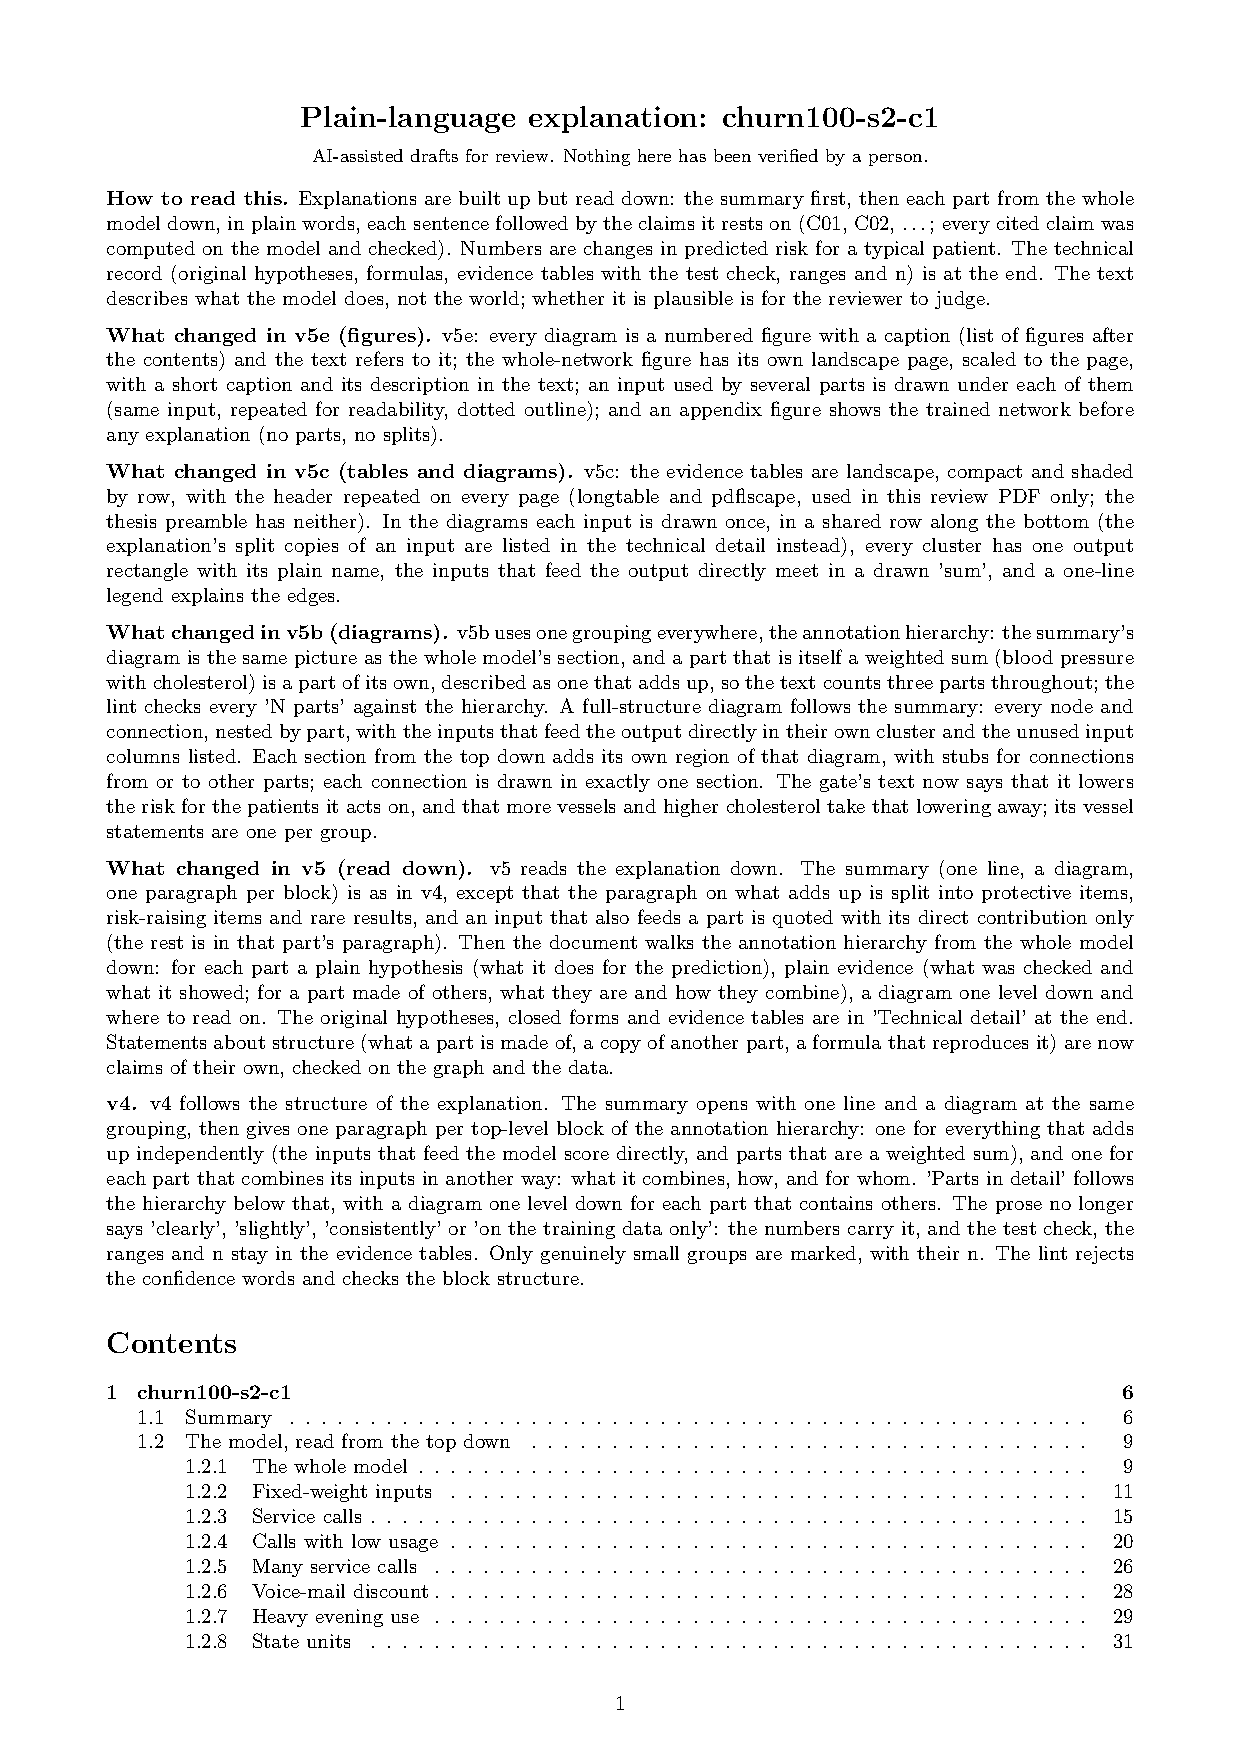
\includepdf[pages={1-7},addtotoc={1,section,1,{churn100-s2-c1: plain-language explanation (read-down document)},plain:churn100-s2-c1}]{churn100-s2-c1/churn100-s2-c1-plain-v5.pdf}
\includepdf[pages={8},landscape]{churn100-s2-c1/churn100-s2-c1-plain-v5.pdf}
\includepdf[pages={9-41}]{churn100-s2-c1/churn100-s2-c1-plain-v5.pdf}
\includepdf[pages={42-44},landscape]{churn100-s2-c1/churn100-s2-c1-plain-v5.pdf}
\includepdf[pages={45}]{churn100-s2-c1/churn100-s2-c1-plain-v5.pdf}
\includepdf[pages={46-48},landscape]{churn100-s2-c1/churn100-s2-c1-plain-v5.pdf}
\includepdf[pages={49}]{churn100-s2-c1/churn100-s2-c1-plain-v5.pdf}
\includepdf[pages={50-51},landscape]{churn100-s2-c1/churn100-s2-c1-plain-v5.pdf}
\includepdf[pages={52}]{churn100-s2-c1/churn100-s2-c1-plain-v5.pdf}
\includepdf[pages={53-54},landscape]{churn100-s2-c1/churn100-s2-c1-plain-v5.pdf}
\includepdf[pages={55}]{churn100-s2-c1/churn100-s2-c1-plain-v5.pdf}
\includepdf[pages={56},landscape]{churn100-s2-c1/churn100-s2-c1-plain-v5.pdf}
\includepdf[pages={57}]{churn100-s2-c1/churn100-s2-c1-plain-v5.pdf}
\includepdf[pages={58},landscape]{churn100-s2-c1/churn100-s2-c1-plain-v5.pdf}
\includepdf[pages={59}]{churn100-s2-c1/churn100-s2-c1-plain-v5.pdf}
\includepdf[pages={60},landscape]{churn100-s2-c1/churn100-s2-c1-plain-v5.pdf}
\includepdf[pages={61}]{churn100-s2-c1/churn100-s2-c1-plain-v5.pdf}
\includepdf[pages={62},landscape]{churn100-s2-c1/churn100-s2-c1-plain-v5.pdf}
\includepdf[pages={63}]{churn100-s2-c1/churn100-s2-c1-plain-v5.pdf}
\includepdf[pages={64},landscape]{churn100-s2-c1/churn100-s2-c1-plain-v5.pdf}
\includepdf[pages={65}]{churn100-s2-c1/churn100-s2-c1-plain-v5.pdf}
\includepdf[pages={66},landscape]{churn100-s2-c1/churn100-s2-c1-plain-v5.pdf}
\includepdf[pages={67}]{churn100-s2-c1/churn100-s2-c1-plain-v5.pdf}
\includepdf[pages={68},landscape]{churn100-s2-c1/churn100-s2-c1-plain-v5.pdf}
\includepdf[pages={69}]{churn100-s2-c1/churn100-s2-c1-plain-v5.pdf}
\addcontentsline{toc}{section}{churn100-s2-c1: coverage certificate}
% Coverage certificate for churn100-s2-c1 (genome f188e353-beb3-4b23-9e19-b64aba8cb5ba); content sha256 e92cc46d5657fbebd82ffc26951bda1ae38642e451964be2a42c3c8e8064f0e4.
\providecommand{\explaneatcertdir}[1]{}
\begin{drafted}[churn100-s2-c1 coverage certificate]
\section{Coverage certificate: churn100-s2-c1}\label{app:churn100-s2-c1:sec}
Provenance, coverage and checks of the explanation, rendered from the canonical JSON record \texttt{churn100-s2-c1.json} (schema 1.4.0, SHA-256 \texttt{e92cc46d5657fbeb}\ldots). The explanation itself (summary, parts, evidence, figures) is the read-down document before this page.

\begin{table}[htbp]
\centering\small
\begin{tabularx}{\linewidth}{@{}lX@{}}
\toprule
Dataset & churn\_\allowbreak{}onehot \\
Experiment & churn100-s2, seed 2 \\
Genome & \texttt{f188e353-beb3-4b23-9e19-b64aba8cb5ba} (NEAT key 24636, generation 99) \\
Explanation & \texttt{6eb705c3-d493-4a02-ab0a-6e01b8c5d696} (103 operations) \\
Train AUC / accuracy & 0.9009 / 0.9008 (n = 4000) \\
Test AUC / accuracy & 0.8756 / 0.901 (n = 1000) \\
Output activation & sigmoid \\
Phenotype & 94 nodes (71 inputs, 22 hidden, 1 output), 95 enabled edges \\
Explained model state & 116 nodes, 100 enabled edges \\
Refactoring operations & add\_\allowbreak{}identity\_\allowbreak{}node 2, consolidate\_\allowbreak{}node 3, split\_\allowbreak{}node 17 \\
Function preservation & max $|\Delta\,\mathrm{output}|$ = $6.66\times 10^{-16}$ on the training split \\
Annotations & 10 (8 leaf, 2 composition) \\
Structural coverage & 1 (115 of 115 candidate nodes; 24 Null) \\
Compositional coverage & 1 \\
Uncovered nodes / edges & 0 / 0 \\
Missing compositions & 0 \\
Full coverage & yes \\
Drafted by & AI-assisted draft \\
Verified by & unverified \\
Record hash (SHA-256) & \texttt{e92cc46d5657fbeb}\ldots \\
\bottomrule
\end{tabularx}
\caption{Explanation certificate summary: churn100-s2-c1.}
\label{app:churn100-s2-c1:summary}
\end{table}
\subsection{Coverage}\label{app:churn100-s2-c1:coverage}
Coverage is computed by the current code (the function behind the \texttt{get\_coverage} tool) under these conventions. \emph{Candidate nodes} are all nodes of the explained model state except the output nodes. A candidate node is \emph{covered} when some annotation of the hierarchy (a leaf, or a composition together with its descendants) contains it and all its enabled outgoing edges. \emph{Exact Null} parts, which have no effect on any output for any input, count as covered: nodes with no path to an output over enabled, non-zero-weight edges (disconnected inputs and dead ends), and edges that have zero weight or touch such a node. Compositional coverage is the fraction of required compositions present: every annotation except a single global root containing every output must have a parent; a parentless, childless annotation made only of Null nodes is exempt.

\begin{itemize}
\item \textbf{Null, disconnected input (24):} \texttt{-10} (state:17), \texttt{-11} (state:18), \texttt{-15} (state:21), \texttt{-16} (state:22), \texttt{-17} (state:23), \texttt{-19} (state:25), \texttt{-26} (state:31), \texttt{-29} (state:34), \texttt{-3} (state:10), \texttt{-34} (state:39), \texttt{-36} (state:40), \texttt{-39} (state:43), \texttt{-49} (state:7), \texttt{-5} (state:12), \texttt{-50} (state:8), \texttt{-51} (state:9), \texttt{-6} (state:13), \texttt{-61} (totalDayCharge), \texttt{-63} (totalEveCalls), \texttt{-67} (totalNightCharge), \texttt{-69} (totalIntlCalls), \texttt{-7} (state:14), \texttt{-8} (state:15), \texttt{-9} (state:16).
\item \textbf{Uncovered nodes:} none.
\item \textbf{Uncovered edges:} none.
\item \textbf{Missing compositions:} none.
\end{itemize}
\noindent\textbf{Agreement with the \texttt{get\_coverage} tool:} yes.

\subsection{Closed-form checks}\label{app:churn100-s2-c1:closedform}
{\small\noindent\begin{tabularx}{\linewidth}{@{}lXrr@{}}
\toprule Tag & Annotation & Closed form vs forward pass & Exact function vs forward pass \\ \midrule
A1 & churn\_\allowbreak{}logit & 0.00582 & $6.66\times 10^{-16}$ \\
A2 & intl\_\allowbreak{}state\_\allowbreak{}unit & 0.00409 & $8.88\times 10^{-16}$ \\
A3 & eve\_\allowbreak{}minutes\_\allowbreak{}hinge & 0.00493 & 0 \\
A4 & voicemail\_\allowbreak{}chain & 0.01 & $4.44\times 10^{-16}$ \\
A5 & state\_\allowbreak{}offsets & 0.0312 & 0 \\
A6 & day\_\allowbreak{}calls\_\allowbreak{}state42 & 0.0035 & 0 \\
A7 & linear\_\allowbreak{}backbone & 0.0152 & $2.66\times 10^{-15}$ \\
A8 & service\_\allowbreak{}call\_\allowbreak{}nonlinear & 0.0274 & $3.55\times 10^{-15}$ \\
A9 & csc\_\allowbreak{}usage\_\allowbreak{}gate & 0.0119 & $8.88\times 10^{-16}$ \\
A10 & csc\_\allowbreak{}hinge & 0.00181 & $4.44\times 10^{-16}$ \\
\bottomrule
\end{tabularx}\par}
\subsection{Refactoring operations}\label{app:churn100-s2-c1:operations}
The explained model state is the phenotype after these operations, replayed in order. All are function-preserving; the largest change in the model output over the 4000 training rows is $6.66\times 10^{-16}$ (tolerance $1.00\times 10^{-9}$).
\begin{itemize}
\item \#71: split \texttt{2627} into \texttt{2627\_\allowbreak{}a}, \texttt{2627\_\allowbreak{}b}.
\item \#72: split \texttt{9555} into \texttt{9555\_\allowbreak{}a}, \texttt{9555\_\allowbreak{}b}.
\item \#73: split \texttt{-71} into \texttt{-71\_\allowbreak{}a}, \texttt{-71\_\allowbreak{}b}, \texttt{-71\_\allowbreak{}c}, \texttt{-71\_\allowbreak{}d}, \texttt{-71\_\allowbreak{}e}, \texttt{-71\_\allowbreak{}f}, \texttt{-71\_\allowbreak{}g}, \texttt{-71\_\allowbreak{}h}.
\item \#74: split \texttt{-70} into \texttt{-70\_\allowbreak{}a}, \texttt{-70\_\allowbreak{}b}, \texttt{-70\_\allowbreak{}c}.
\item \#75: split \texttt{-64} into \texttt{-64\_\allowbreak{}a}, \texttt{-64\_\allowbreak{}b}.
\item \#76: split \texttt{-62} into \texttt{-62\_\allowbreak{}a}, \texttt{-62\_\allowbreak{}b}.
\item \#77: split \texttt{-60} into \texttt{-60\_\allowbreak{}a}, \texttt{-60\_\allowbreak{}b}.
\item \#78: split \texttt{-59} into \texttt{-59\_\allowbreak{}a}, \texttt{-59\_\allowbreak{}b}.
\item \#79: split \texttt{-57} into \texttt{-57\_\allowbreak{}a}, \texttt{-57\_\allowbreak{}b}.
\item \#80: split \texttt{-47} into \texttt{-47\_\allowbreak{}a}, \texttt{-47\_\allowbreak{}b}.
\item \#81: split \texttt{-45} into \texttt{-45\_\allowbreak{}a}, \texttt{-45\_\allowbreak{}b}, \texttt{-45\_\allowbreak{}c}.
\item \#82: split \texttt{-37} into \texttt{-37\_\allowbreak{}a}, \texttt{-37\_\allowbreak{}b}.
\item \#83: split \texttt{-30} into \texttt{-30\_\allowbreak{}a}, \texttt{-30\_\allowbreak{}b}, \texttt{-30\_\allowbreak{}c}, \texttt{-30\_\allowbreak{}d}.
\item \#84: split \texttt{-24} into \texttt{-24\_\allowbreak{}a}, \texttt{-24\_\allowbreak{}b}.
\item \#85: split \texttt{-21} into \texttt{-21\_\allowbreak{}a}, \texttt{-21\_\allowbreak{}b}.
\item \#86: split \texttt{-18} into \texttt{-18\_\allowbreak{}a}, \texttt{-18\_\allowbreak{}b}.
\item \#87: split \texttt{-13} into \texttt{-13\_\allowbreak{}a}, \texttt{-13\_\allowbreak{}b}.
\item \#88: consolidate \texttt{-71\_\allowbreak{}a}, \texttt{-71\_\allowbreak{}b}, \texttt{-71\_\allowbreak{}c}, \texttt{-71\_\allowbreak{}f}, \texttt{-71\_\allowbreak{}h}.
\item \#89: consolidate \texttt{-71\_\allowbreak{}e}, \texttt{-71\_\allowbreak{}g}.
\item \#90: consolidate \texttt{-30\_\allowbreak{}b}, \texttt{-30\_\allowbreak{}c}, \texttt{-30\_\allowbreak{}d}.
\item \#98: identity node \texttt{identity\_\allowbreak{}lin} before \texttt{0} (40 connection(s)).
\item \#100: identity node \texttt{identity\_\allowbreak{}svc} before \texttt{0} (3 connection(s)).
\end{itemize}
\subsection{Audit against the definitions}\label{app:churn100-s2-c1:audit}
Automatic findings on the stored explanation (codes as in the JSON record's \texttt{issues}); they flag what an examiner should check, not verdicts.
\begin{itemize}
\item \textsc{warning} \texttt{unverified}: No human verification is recorded for this explanation.
\end{itemize}
\end{drafted}

\clearpage
\section*{2. churn100-s2-c2: verification checklist}
\addcontentsline{toc}{section}{2. churn100-s2-c2: verification checklist}
\label{rev:churn100-s2-c2}
\textbf{Already recorded:} nothing (no verdict in the record).

\textbf{Recorded vs live.} Agent = the drafting agent's report; orchestrator = the record's automated re-check; live = this export (current code, training split).

{\footnotesize
\begin{tabularx}{\linewidth}{@{}>{\raggedright\arraybackslash}X>{\raggedright\arraybackslash}p{2.1cm}>{\raggedright\arraybackslash}p{3.0cm}>{\raggedright\arraybackslash}p{3.0cm}l@{}}
\toprule
Check & Agent & Orchestrator & Live & Status \\
\midrule
Function preservation, max $|$change in output$|$ & 5.55e-16 & 5.55e-16 & 5.55e-16 & agree \\
Closed-form max abs error (all leaves) & 0.04264 & 0.04264 & 0.04264 & agree \\
Numeric-function max abs error & n/a & 2.66e-15 & 2.66e-15 & agree \\
Structural coverage & 1 & 1 & 1 & agree \\
Compositional coverage & 1 & 1 & 1 & agree \\
Hierarchy complete & yes & yes & yes & agree \\
Root annotation & n/a & churn\_\allowbreak{}logit & churn\_\allowbreak{}logit & agree \\
Leaf / composition counts & 7 / 2 & n/a & 7 / 2 & agree \\
Operation counts & 13 splits, 2 identity & add identity node 2, annotate 9, consolidate node 3, rename node 71, split node 13 & add identity node 2, annotate 9, consolidate node 3, rename node 71, split node 13 & agree \\
Full coverage & yes & yes & yes & agree \\
\bottomrule
\end{tabularx}}

\textbf{What to look at.}
\begin{itemize}
\item Largest closed-form error: \texttt{state\_\allowbreak{}offsets} (0.0426), then \texttt{linear\_\allowbreak{}backbone} (0.0165). This is the cost of the 3 s.f. display rounding, in the exit's own units; the numeric function is exact. Check that the rounded formula still supports the hypothesis as worded.
\item Strong claim in \texttt{csc\_\allowbreak{}usage\_\allowbreak{}gate}: \emph{``Mean churn by calls 0-6: 0.115/\allowbreak{}0.110/\allowbreak{}0.110/\allowbreak{}0.106/\allowbreak{}0.437/\allowbreak{}0.571/\allowbreak{}0.679,\allowbreak{} model 0.087/\allowbreak{}0.078/\allowbreak{}0.080/\allowbreak{}0.113/\allowbreak{}0.246/\allowbreak{}0.503/\allowbreak{}0.820;\allowbreak{}''} Is this (exactness, threshold, rare category) supported by the evidence, or fitted to a few rows?
\item Strong claim in \texttt{area\_\allowbreak{}code\_\allowbreak{}units}: \emph{``161 = relu(-0.14 + 0.58 areaCode:415), logit weight +0.05: on exactly for area code 415 (binary), so exactly affine (+0.02 logit for area code 415).''} Is this (exactness, threshold, rare category) supported by the evidence, or fitted to a few rows?
\item 13 split(s), all of input nodes (an input feeding two annotations). These are routine; check only that each input copy sits in the annotation whose hypothesis uses it.
\item 3 consolidation(s): copies merged back after a split. Check that the merged copies carry the same role.
\item Read the root's hypothesis against its closed form: does the stated combination of children (additive, gated, serial) match the formula?
\end{itemize}
\textbf{Tool notes (record):} None new. Following the sibling agent's note, all splits were input splits before consolidation (no hidden split was needed). The Bash sandbox refused shell loops/\allowbreak{}variables/\allowbreak{}heredocs around uv, so tool calls were driven from a scratch Python script that runs experiments/\allowbreak{}species\_\allowbreak{}leads/\allowbreak{}xn.py per call (all calls logged).

\textbf{Plain-language layer} (AI-assisted draft for review (unverified)): the read-down document follows this page (summary, parts, evidence, worth checking; also \texttt{churn100-s2-c2-plain-v5.pdf} in this genome's folder). Record a verdict on it with \texttt{uv run python -m explaneat export record-plain-verdict churn100-s2-c2 --verified --minutes N --notes "..."}.

\textbf{Verdict.}

\begin{tabularx}{\linewidth}{@{}lX@{}}
Verified (correct as it stands, or after my changes): & $\square$ yes \quad $\square$ no \\[4pt]
Minutes: & \rule{3cm}{0.4pt} \\[4pt]
Changes: & \rule{\linewidth}{0.4pt} \\[10pt]
 & \rule{\linewidth}{0.4pt} \\[4pt]
Notes: & \rule{\linewidth}{0.4pt} \\[10pt]
 & \rule{\linewidth}{0.4pt} \\
\end{tabularx}

\textbf{Record it} (writes \texttt{mike\_verification} into \texttt{experiments/10seed/explanations/churn100-s2-c2.json}; use \texttt{-{}-not-verified} for no; rebuild the CSVs with \texttt{uv run python experiments/10seed/build\_explanations\_csv.py}):

{\footnotesize\raggedright\texttt{uv run python -m explaneat export record-verdict churn100-s2-c2 --verified --minutes N --changes "..." --notes "..."}\par}


\clearpage
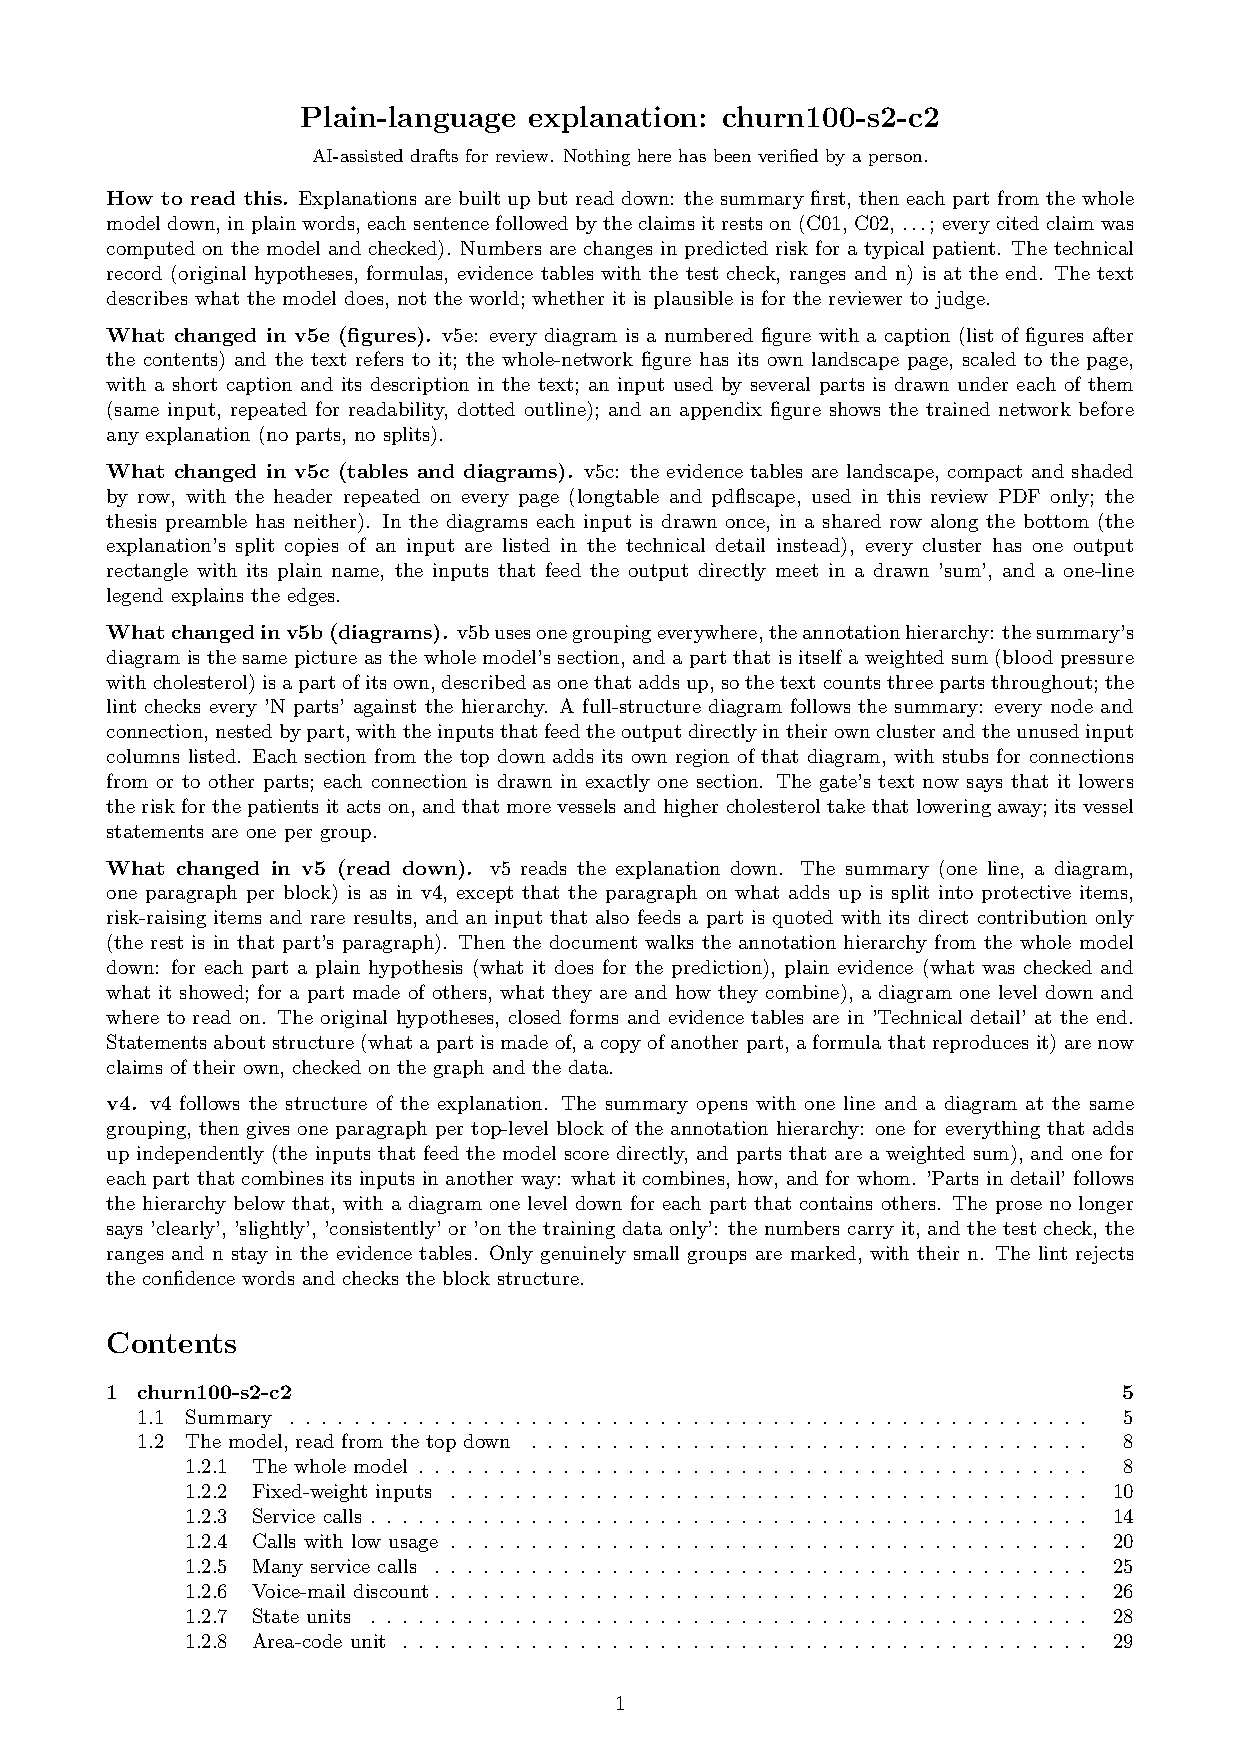
\includepdf[pages={1-6},addtotoc={1,section,1,{churn100-s2-c2: plain-language explanation (read-down document)},plain:churn100-s2-c2}]{churn100-s2-c2/churn100-s2-c2-plain-v5.pdf}
\includepdf[pages={7},landscape]{churn100-s2-c2/churn100-s2-c2-plain-v5.pdf}
\includepdf[pages={8-34}]{churn100-s2-c2/churn100-s2-c2-plain-v5.pdf}
\includepdf[pages={35-37},landscape]{churn100-s2-c2/churn100-s2-c2-plain-v5.pdf}
\includepdf[pages={38}]{churn100-s2-c2/churn100-s2-c2-plain-v5.pdf}
\includepdf[pages={39-40},landscape]{churn100-s2-c2/churn100-s2-c2-plain-v5.pdf}
\includepdf[pages={41}]{churn100-s2-c2/churn100-s2-c2-plain-v5.pdf}
\includepdf[pages={42-43},landscape]{churn100-s2-c2/churn100-s2-c2-plain-v5.pdf}
\includepdf[pages={44}]{churn100-s2-c2/churn100-s2-c2-plain-v5.pdf}
\includepdf[pages={45-46},landscape]{churn100-s2-c2/churn100-s2-c2-plain-v5.pdf}
\includepdf[pages={47}]{churn100-s2-c2/churn100-s2-c2-plain-v5.pdf}
\includepdf[pages={48},landscape]{churn100-s2-c2/churn100-s2-c2-plain-v5.pdf}
\includepdf[pages={49}]{churn100-s2-c2/churn100-s2-c2-plain-v5.pdf}
\includepdf[pages={50},landscape]{churn100-s2-c2/churn100-s2-c2-plain-v5.pdf}
\includepdf[pages={51}]{churn100-s2-c2/churn100-s2-c2-plain-v5.pdf}
\includepdf[pages={52},landscape]{churn100-s2-c2/churn100-s2-c2-plain-v5.pdf}
\includepdf[pages={53}]{churn100-s2-c2/churn100-s2-c2-plain-v5.pdf}
\includepdf[pages={54},landscape]{churn100-s2-c2/churn100-s2-c2-plain-v5.pdf}
\includepdf[pages={55}]{churn100-s2-c2/churn100-s2-c2-plain-v5.pdf}
\includepdf[pages={56},landscape]{churn100-s2-c2/churn100-s2-c2-plain-v5.pdf}
\includepdf[pages={57}]{churn100-s2-c2/churn100-s2-c2-plain-v5.pdf}
\includepdf[pages={58},landscape]{churn100-s2-c2/churn100-s2-c2-plain-v5.pdf}
\includepdf[pages={59}]{churn100-s2-c2/churn100-s2-c2-plain-v5.pdf}
\addcontentsline{toc}{section}{churn100-s2-c2: coverage certificate}
% Coverage certificate for churn100-s2-c2 (genome e5394267-5807-44ae-8629-5e157bcfb43a); content sha256 3994ace43ba746828471d4467bcb28a9e464f2912f95c9ca149d67f70e20f448.
\providecommand{\explaneatcertdir}[1]{}
\begin{drafted}[churn100-s2-c2 coverage certificate]
\section{Coverage certificate: churn100-s2-c2}\label{app:churn100-s2-c2:sec}
Provenance, coverage and checks of the explanation, rendered from the canonical JSON record \texttt{churn100-s2-c2.json} (schema 1.4.0, SHA-256 \texttt{3994ace43ba74682}\ldots). The explanation itself (summary, parts, evidence, figures) is the read-down document before this page.

\begin{table}[htbp]
\centering\small
\begin{tabularx}{\linewidth}{@{}lX@{}}
\toprule
Dataset & churn\_\allowbreak{}onehot \\
Experiment & churn100-s2, seed 2 \\
Genome & \texttt{e5394267-5807-44ae-8629-5e157bcfb43a} (NEAT key 24564, generation 99) \\
Explanation & \texttt{4792056e-ee3e-4fde-a1bb-4c4d809e2d61} (98 operations) \\
Train AUC / accuracy & 0.8944 / 0.896 (n = 4000) \\
Test AUC / accuracy & 0.8883 / 0.9 (n = 1000) \\
Output activation & sigmoid \\
Phenotype & 97 nodes (71 inputs, 25 hidden, 1 output), 89 enabled edges \\
Explained model state & 114 nodes, 91 enabled edges \\
Refactoring operations & add\_\allowbreak{}identity\_\allowbreak{}node 2, consolidate\_\allowbreak{}node 3, split\_\allowbreak{}node 13 \\
Function preservation & max $|\Delta\,\mathrm{output}|$ = $5.55\times 10^{-16}$ on the training split \\
Annotations & 9 (7 leaf, 2 composition) \\
Structural coverage & 1 (113 of 113 candidate nodes; 30 Null) \\
Compositional coverage & 1 \\
Uncovered nodes / edges & 0 / 0 \\
Missing compositions & 0 \\
Full coverage & yes \\
Drafted by & AI-assisted draft \\
Verified by & unverified \\
Record hash (SHA-256) & \texttt{3994ace43ba74682}\ldots \\
\bottomrule
\end{tabularx}
\caption{Explanation certificate summary: churn100-s2-c2.}
\label{app:churn100-s2-c2:summary}
\end{table}
\subsection{Coverage}\label{app:churn100-s2-c2:coverage}
Coverage is computed by the current code (the function behind the \texttt{get\_coverage} tool) under these conventions. \emph{Candidate nodes} are all nodes of the explained model state except the output nodes. A candidate node is \emph{covered} when some annotation of the hierarchy (a leaf, or a composition together with its descendants) contains it and all its enabled outgoing edges. \emph{Exact Null} parts, which have no effect on any output for any input, count as covered: nodes with no path to an output over enabled, non-zero-weight edges (disconnected inputs and dead ends), and edges that have zero weight or touch such a node. Compositional coverage is the fraction of required compositions present: every annotation except a single global root containing every output must have a parent; a parentless, childless annotation made only of Null nodes is exempt.

\begin{itemize}
\item \textbf{Null, disconnected input (30):} \texttt{-11} (state:18), \texttt{-13} (state:2), \texttt{-15} (state:21), \texttt{-16} (state:22), \texttt{-19} (state:25), \texttt{-2} (state:1), \texttt{-23} (state:29), \texttt{-25} (state:30), \texttt{-26} (state:31), \texttt{-27} (state:32), \texttt{-29} (state:34), \texttt{-3} (state:10), \texttt{-33} (state:38), \texttt{-34} (state:39), \texttt{-38} (state:42), \texttt{-42} (state:46), \texttt{-44} (state:48), \texttt{-46} (state:5), \texttt{-47} (state:50), \texttt{-48} (state:6), \texttt{-5} (state:12), \texttt{-51} (state:9), \texttt{-6} (state:13), \texttt{-61} (totalDayCharge), \texttt{-63} (totalEveCalls), \texttt{-66} (totalNightCalls), \texttt{-67} (totalNightCharge), \texttt{-68} (totalIntlMinutes), \texttt{-7} (state:14), \texttt{-9} (state:16).
\item \textbf{Uncovered nodes:} none.
\item \textbf{Uncovered edges:} none.
\item \textbf{Missing compositions:} none.
\end{itemize}
\noindent\textbf{Agreement with the \texttt{get\_coverage} tool:} yes.

\subsection{Closed-form checks}\label{app:churn100-s2-c2:closedform}
{\small\noindent\begin{tabularx}{\linewidth}{@{}lXrr@{}}
\toprule Tag & Annotation & Closed form vs forward pass & Exact function vs forward pass \\ \midrule
A1 & churn\_\allowbreak{}logit & 0.00617 & $8.88\times 10^{-16}$ \\
A2 & linear\_\allowbreak{}backbone & 0.0165 & $2.66\times 10^{-15}$ \\
A3 & voicemail\_\allowbreak{}chain & 0.00153 & $4.44\times 10^{-16}$ \\
A4 & intl\_\allowbreak{}state44\_\allowbreak{}unit & 0.008 & 0 \\
A5 & area\_\allowbreak{}code\_\allowbreak{}units & $3.38\times 10^{-4}$ & 0 \\
A6 & state\_\allowbreak{}offsets & 0.0426 & 0 \\
A7 & service\_\allowbreak{}call\_\allowbreak{}nonlinear & 0.0374 & $3.55\times 10^{-15}$ \\
A8 & csc\_\allowbreak{}usage\_\allowbreak{}gate & 0.0112 & $8.88\times 10^{-16}$ \\
A9 & csc\_\allowbreak{}hinge & 0.00224 & 0 \\
\bottomrule
\end{tabularx}\par}
\subsection{Refactoring operations}\label{app:churn100-s2-c2:operations}
The explained model state is the phenotype after these operations, replayed in order. All are function-preserving; the largest change in the model output over the 4000 training rows is $5.55\times 10^{-16}$ (tolerance $1.00\times 10^{-9}$).
\begin{itemize}
\item \#71: split \texttt{-71} into \texttt{-71\_\allowbreak{}a}, \texttt{-71\_\allowbreak{}b}, \texttt{-71\_\allowbreak{}c}, \texttt{-71\_\allowbreak{}d}, \texttt{-71\_\allowbreak{}e}.
\item \#72: split \texttt{-70} into \texttt{-70\_\allowbreak{}a}, \texttt{-70\_\allowbreak{}b}, \texttt{-70\_\allowbreak{}c}.
\item \#73: split \texttt{-64} into \texttt{-64\_\allowbreak{}a}, \texttt{-64\_\allowbreak{}b}.
\item \#74: split \texttt{-59} into \texttt{-59\_\allowbreak{}a}, \texttt{-59\_\allowbreak{}b}.
\item \#75: split \texttt{-57} into \texttt{-57\_\allowbreak{}a}, \texttt{-57\_\allowbreak{}b}, \texttt{-57\_\allowbreak{}c}, \texttt{-57\_\allowbreak{}d}.
\item \#76: split \texttt{-43} into \texttt{-43\_\allowbreak{}a}, \texttt{-43\_\allowbreak{}b}, \texttt{-43\_\allowbreak{}c}.
\item \#77: split \texttt{-37} into \texttt{-37\_\allowbreak{}a}, \texttt{-37\_\allowbreak{}b}.
\item \#78: split \texttt{-28} into \texttt{-28\_\allowbreak{}a}, \texttt{-28\_\allowbreak{}b}.
\item \#79: split \texttt{-24} into \texttt{-24\_\allowbreak{}a}, \texttt{-24\_\allowbreak{}b}.
\item \#80: split \texttt{-22} into \texttt{-22\_\allowbreak{}a}, \texttt{-22\_\allowbreak{}b}.
\item \#81: split \texttt{-21} into \texttt{-21\_\allowbreak{}a}, \texttt{-21\_\allowbreak{}b}.
\item \#82: split \texttt{-20} into \texttt{-20\_\allowbreak{}a}, \texttt{-20\_\allowbreak{}b}, \texttt{-20\_\allowbreak{}c}.
\item \#83: split \texttt{-1} into \texttt{-1\_\allowbreak{}a}, \texttt{-1\_\allowbreak{}b}.
\item \#84: consolidate \texttt{-71\_\allowbreak{}a}, \texttt{-71\_\allowbreak{}b}, \texttt{-71\_\allowbreak{}d}, \texttt{-71\_\allowbreak{}e}.
\item \#85: consolidate \texttt{-57\_\allowbreak{}b}, \texttt{-57\_\allowbreak{}c}, \texttt{-57\_\allowbreak{}d}.
\item \#86: consolidate \texttt{-20\_\allowbreak{}b}, \texttt{-20\_\allowbreak{}c}.
\item \#87: identity node \texttt{identity\_\allowbreak{}lin} before \texttt{0} (33 connection(s)).
\item \#88: identity node \texttt{identity\_\allowbreak{}svc} before \texttt{0} (3 connection(s)).
\end{itemize}
\subsection{Audit against the definitions}\label{app:churn100-s2-c2:audit}
Automatic findings on the stored explanation (codes as in the JSON record's \texttt{issues}); they flag what an examiner should check, not verdicts.
\begin{itemize}
\item \textsc{warning} \texttt{unverified}: No human verification is recorded for this explanation.
\end{itemize}
\end{drafted}

\clearpage
\section*{3. churn100-s4-c2: verification checklist}
\addcontentsline{toc}{section}{3. churn100-s4-c2: verification checklist}
\label{rev:churn100-s4-c2}
\textbf{Already recorded:} nothing (no verdict in the record).

\textbf{Recorded vs live.} Agent = the drafting agent's report; orchestrator = the record's automated re-check; live = this export (current code, training split).

{\footnotesize
\begin{tabularx}{\linewidth}{@{}>{\raggedright\arraybackslash}X>{\raggedright\arraybackslash}p{2.1cm}>{\raggedright\arraybackslash}p{3.0cm}>{\raggedright\arraybackslash}p{3.0cm}l@{}}
\toprule
Check & Agent & Orchestrator & Live & Status \\
\midrule
Function preservation, max $|$change in output$|$ & 4.44e-16 & 4.44e-16 & 4.44e-16 & agree \\
Closed-form max abs error (all leaves) & 0.01996 & 0.01996 & 0.01996 & agree \\
Numeric-function max abs error & n/a & 1.78e-15 & 1.78e-15 & agree \\
Structural coverage & 1 & 1 & 1 & agree \\
Compositional coverage & 1 & 1 & 1 & agree \\
Hierarchy complete & yes & yes & yes & agree \\
Root annotation & n/a & churn\_\allowbreak{}logit & churn\_\allowbreak{}logit & agree \\
Leaf / composition counts & 7 / 2 & n/a & 7 / 2 & agree \\
Operation counts & 5 splits, 2 identity & add identity node 2, annotate 9, consolidate node 1, rename node 71, split node 5 & add identity node 2, annotate 9, consolidate node 1, rename node 71, split node 5 & agree \\
Full coverage & yes & yes & yes & agree \\
\bottomrule
\end{tabularx}}

\textbf{What to look at.}
\begin{itemize}
\item Largest closed-form error: \texttt{vmail\_\allowbreak{}state18\_\allowbreak{}unit} (0.02), then \texttt{evening\_\allowbreak{}hinge} (0.0165). This is the cost of the 3 s.f. display rounding, in the exit's own units; the numeric function is exact. Check that the rounded formula still supports the hypothesis as worded.
\item Strong claim in \texttt{csc\_\allowbreak{}high\_\allowbreak{}hinge}: \emph{``Active on exactly the 8\% of customers with 4+ calls (318 rows;''} Is this (exactness, threshold, rare category) supported by the evidence, or fitted to a few rows?
\item Strong claim in \texttt{state\_\allowbreak{}offsets}: \emph{``Each depends only on one binary state indicator, so each is exactly an offset (least-squares R2 = 1.0).''} Is this (exactness, threshold, rare category) supported by the evidence, or fitted to a few rows?
\item 5 split(s), all of input nodes (an input feeding two annotations). These are routine; check only that each input copy sits in the annotation whose hypothesis uses it.
\item 1 consolidation(s): copies merged back after a split. Check that the merged copies carry the same role.
\item Read the root's hypothesis against its closed form: does the stated combination of children (additive, gated, serial) match the formula?
\end{itemize}
\textbf{Tool notes (record):} None new. Hidden-node splits were not needed; input splits were done before the one consolidation. Display name of the consolidated copy -71\_\allowbreak{}acd is None (cosmetic). Tool calls driven from scratch Python scripts that run experiments/\allowbreak{}species\_\allowbreak{}leads/\allowbreak{}xn.py per call (all logged), because the Bash sandbox refuses shell variables/loops around uv.

\textbf{Plain-language layer} (AI-assisted draft for review (unverified)): the read-down document follows this page (summary, parts, evidence, worth checking; also \texttt{churn100-s4-c2-plain-v5.pdf} in this genome's folder). Record a verdict on it with \texttt{uv run python -m explaneat export record-plain-verdict churn100-s4-c2 --verified --minutes N --notes "..."}.

\textbf{Verdict.}

\begin{tabularx}{\linewidth}{@{}lX@{}}
Verified (correct as it stands, or after my changes): & $\square$ yes \quad $\square$ no \\[4pt]
Minutes: & \rule{3cm}{0.4pt} \\[4pt]
Changes: & \rule{\linewidth}{0.4pt} \\[10pt]
 & \rule{\linewidth}{0.4pt} \\[4pt]
Notes: & \rule{\linewidth}{0.4pt} \\[10pt]
 & \rule{\linewidth}{0.4pt} \\
\end{tabularx}

\textbf{Record it} (writes \texttt{mike\_verification} into \texttt{experiments/10seed/explanations/churn100-s4-c2.json}; use \texttt{-{}-not-verified} for no; rebuild the CSVs with \texttt{uv run python experiments/10seed/build\_explanations\_csv.py}):

{\footnotesize\raggedright\texttt{uv run python -m explaneat export record-verdict churn100-s4-c2 --verified --minutes N --changes "..." --notes "..."}\par}


\clearpage
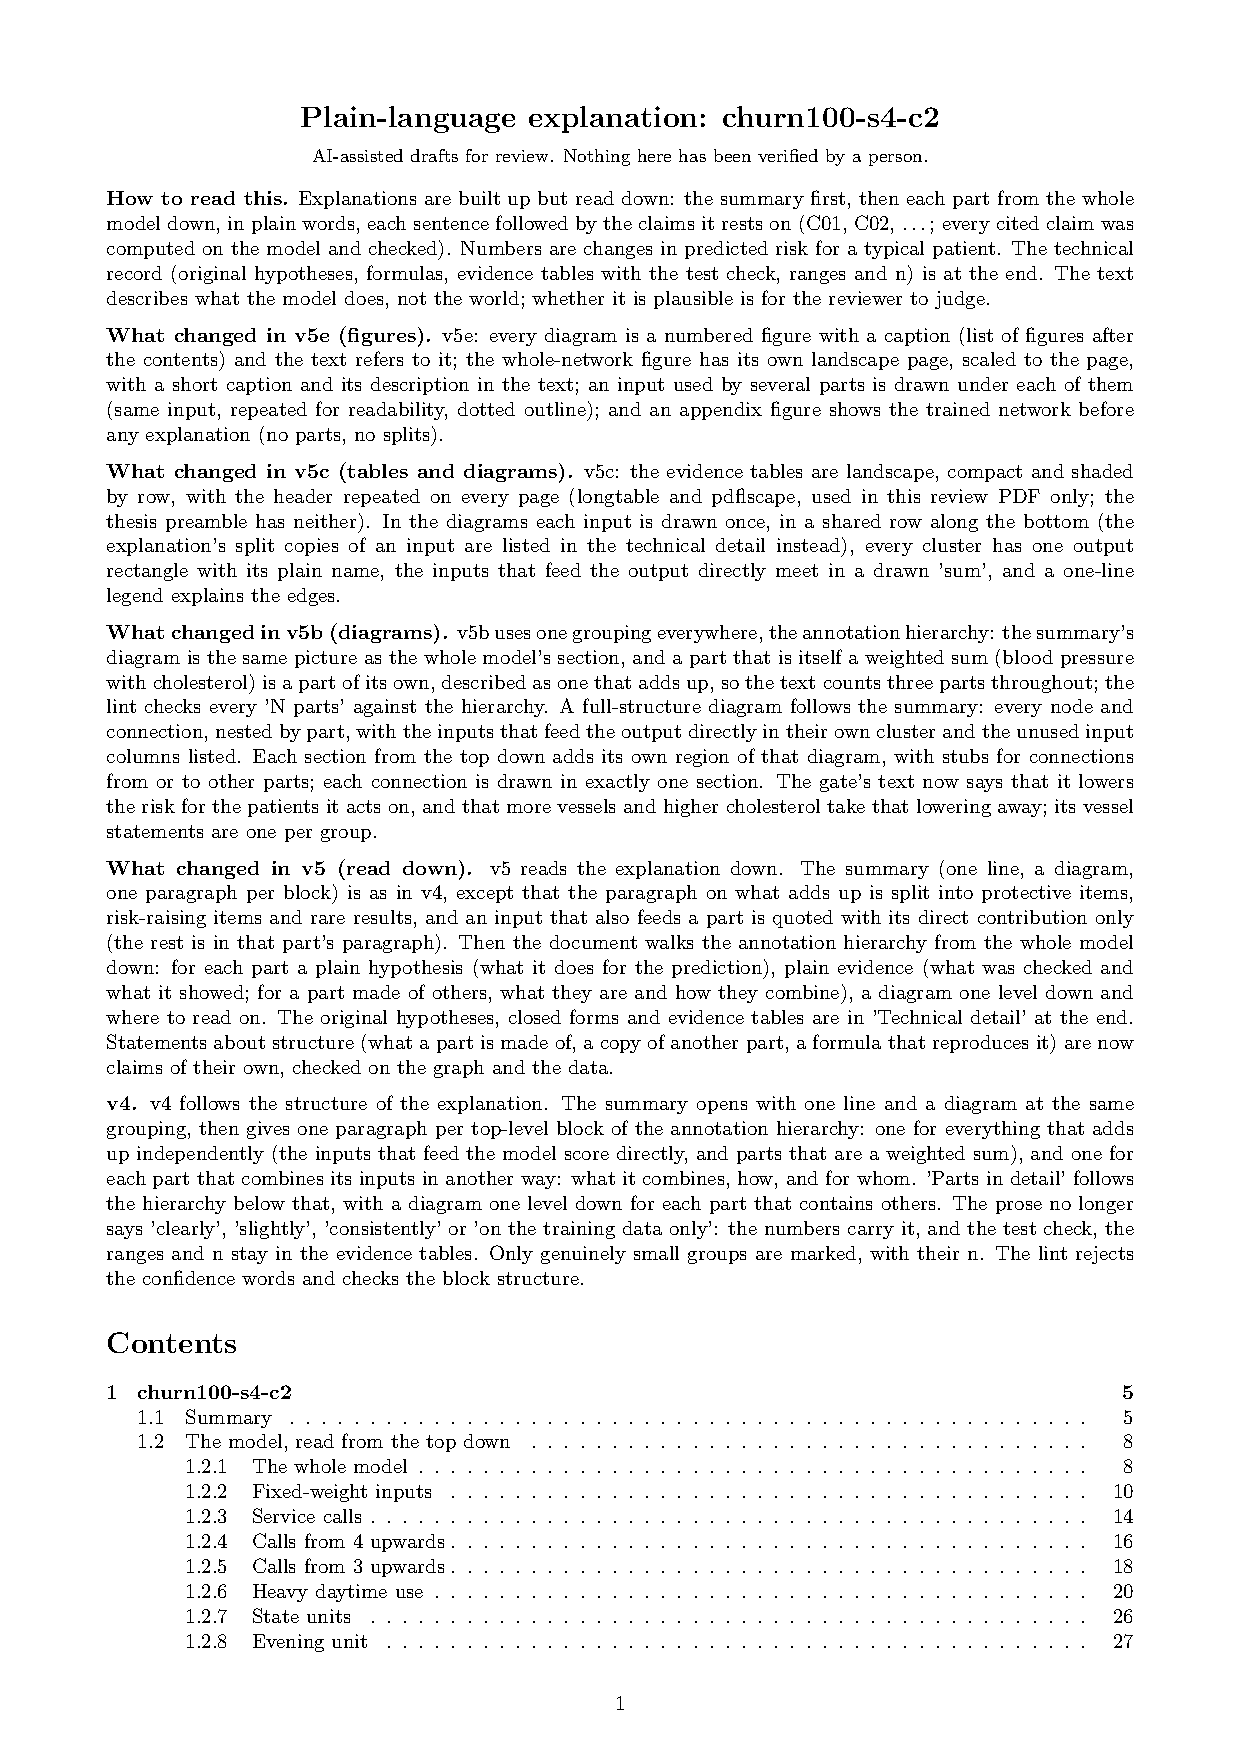
\includepdf[pages={1-6},addtotoc={1,section,1,{churn100-s4-c2: plain-language explanation (read-down document)},plain:churn100-s4-c2}]{churn100-s4-c2/churn100-s4-c2-plain-v5.pdf}
\includepdf[pages={7},landscape]{churn100-s4-c2/churn100-s4-c2-plain-v5.pdf}
\includepdf[pages={8-32}]{churn100-s4-c2/churn100-s4-c2-plain-v5.pdf}
\includepdf[pages={33-35},landscape]{churn100-s4-c2/churn100-s4-c2-plain-v5.pdf}
\includepdf[pages={36}]{churn100-s4-c2/churn100-s4-c2-plain-v5.pdf}
\includepdf[pages={37-38},landscape]{churn100-s4-c2/churn100-s4-c2-plain-v5.pdf}
\includepdf[pages={39}]{churn100-s4-c2/churn100-s4-c2-plain-v5.pdf}
\includepdf[pages={40},landscape]{churn100-s4-c2/churn100-s4-c2-plain-v5.pdf}
\includepdf[pages={41}]{churn100-s4-c2/churn100-s4-c2-plain-v5.pdf}
\includepdf[pages={42},landscape]{churn100-s4-c2/churn100-s4-c2-plain-v5.pdf}
\includepdf[pages={43}]{churn100-s4-c2/churn100-s4-c2-plain-v5.pdf}
\includepdf[pages={44},landscape]{churn100-s4-c2/churn100-s4-c2-plain-v5.pdf}
\includepdf[pages={45}]{churn100-s4-c2/churn100-s4-c2-plain-v5.pdf}
\includepdf[pages={46-47},landscape]{churn100-s4-c2/churn100-s4-c2-plain-v5.pdf}
\includepdf[pages={48}]{churn100-s4-c2/churn100-s4-c2-plain-v5.pdf}
\includepdf[pages={49},landscape]{churn100-s4-c2/churn100-s4-c2-plain-v5.pdf}
\includepdf[pages={50}]{churn100-s4-c2/churn100-s4-c2-plain-v5.pdf}
\includepdf[pages={51},landscape]{churn100-s4-c2/churn100-s4-c2-plain-v5.pdf}
\includepdf[pages={52}]{churn100-s4-c2/churn100-s4-c2-plain-v5.pdf}
\includepdf[pages={53},landscape]{churn100-s4-c2/churn100-s4-c2-plain-v5.pdf}
\includepdf[pages={54}]{churn100-s4-c2/churn100-s4-c2-plain-v5.pdf}
\includepdf[pages={55},landscape]{churn100-s4-c2/churn100-s4-c2-plain-v5.pdf}
\includepdf[pages={56}]{churn100-s4-c2/churn100-s4-c2-plain-v5.pdf}
\addcontentsline{toc}{section}{churn100-s4-c2: coverage certificate}
% Coverage certificate for churn100-s4-c2 (genome 4206744f-b5ce-4488-bc53-a39aa08fe972); content sha256 36f617b704b0542df58a0d74728f2b2ac784fcbc7a36644bcc7c6a2f886b5ed1.
\providecommand{\explaneatcertdir}[1]{}
\begin{drafted}[churn100-s4-c2 coverage certificate]
\section{Coverage certificate: churn100-s4-c2}\label{app:churn100-s4-c2:sec}
Provenance, coverage and checks of the explanation, rendered from the canonical JSON record \texttt{churn100-s4-c2.json} (schema 1.4.0, SHA-256 \texttt{36f617b704b0542d}\ldots). The explanation itself (summary, parts, evidence, figures) is the read-down document before this page.

\begin{table}[htbp]
\centering\small
\begin{tabularx}{\linewidth}{@{}lX@{}}
\toprule
Dataset & churn\_\allowbreak{}onehot \\
Experiment & churn100-s4, seed 4 \\
Genome & \texttt{4206744f-b5ce-4488-bc53-a39aa08fe972} (NEAT key 24427, generation 99) \\
Explanation & \texttt{33d6db5d-fbdf-41c8-a597-fc997715b92f} (88 operations) \\
Train AUC / accuracy & 0.8908 / 0.888 (n = 4000) \\
Test AUC / accuracy & 0.8664 / 0.898 (n = 1000) \\
Output activation & sigmoid \\
Phenotype & 85 nodes (71 inputs, 13 hidden, 1 output), 58 enabled edges \\
Explained model state & 93 nodes, 60 enabled edges \\
Refactoring operations & add\_\allowbreak{}identity\_\allowbreak{}node 2, consolidate\_\allowbreak{}node 1, split\_\allowbreak{}node 5 \\
Function preservation & max $|\Delta\,\mathrm{output}|$ = $4.44\times 10^{-16}$ on the training split \\
Annotations & 9 (7 leaf, 2 composition) \\
Structural coverage & 1 (92 of 92 candidate nodes; 37 Null) \\
Compositional coverage & 1 \\
Uncovered nodes / edges & 0 / 0 \\
Missing compositions & 0 \\
Full coverage & yes \\
Drafted by & AI-assisted draft \\
Verified by & unverified \\
Record hash (SHA-256) & \texttt{36f617b704b0542d}\ldots \\
\bottomrule
\end{tabularx}
\caption{Explanation certificate summary: churn100-s4-c2.}
\label{app:churn100-s4-c2:summary}
\end{table}
\subsection{Coverage}\label{app:churn100-s4-c2:coverage}
Coverage is computed by the current code (the function behind the \texttt{get\_coverage} tool) under these conventions. \emph{Candidate nodes} are all nodes of the explained model state except the output nodes. A candidate node is \emph{covered} when some annotation of the hierarchy (a leaf, or a composition together with its descendants) contains it and all its enabled outgoing edges. \emph{Exact Null} parts, which have no effect on any output for any input, count as covered: nodes with no path to an output over enabled, non-zero-weight edges (disconnected inputs and dead ends), and edges that have zero weight or touch such a node. Compositional coverage is the fraction of required compositions present: every annotation except a single global root containing every output must have a parent; a parentless, childless annotation made only of Null nodes is exempt.

\begin{itemize}
\item \textbf{Null, disconnected input (37):} \texttt{-1} (state:0), \texttt{-14} (state:20), \texttt{-15} (state:21), \texttt{-16} (state:22), \texttt{-17} (state:23), \texttt{-18} (state:24), \texttt{-19} (state:25), \texttt{-2} (state:1), \texttt{-20} (state:26), \texttt{-21} (state:27), \texttt{-23} (state:29), \texttt{-25} (state:30), \texttt{-27} (state:32), \texttt{-28} (state:33), \texttt{-29} (state:34), \texttt{-30} (state:35), \texttt{-35} (state:4), \texttt{-36} (state:40), \texttt{-39} (state:43), \texttt{-40} (state:44), \texttt{-44} (state:48), \texttt{-46} (state:5), \texttt{-47} (state:50), \texttt{-49} (state:7), \texttt{-5} (state:12), \texttt{-50} (state:8), \texttt{-53} (areaCode:408), \texttt{-55} (areaCode:510), \texttt{-6} (state:13), \texttt{-63} (totalEveCalls), \texttt{-65} (totalNightMinutes), \texttt{-66} (totalNightCalls), \texttt{-67} (totalNightCharge), \texttt{-69} (totalIntlCalls), \texttt{-7} (state:14), \texttt{-70} (totalIntlCharge), \texttt{-9} (state:16).
\item \textbf{Uncovered nodes:} none.
\item \textbf{Uncovered edges:} none.
\item \textbf{Missing compositions:} none.
\end{itemize}
\noindent\textbf{Agreement with the \texttt{get\_coverage} tool:} yes.

\subsection{Closed-form checks}\label{app:churn100-s4-c2:closedform}
{\small\noindent\begin{tabularx}{\linewidth}{@{}lXrr@{}}
\toprule Tag & Annotation & Closed form vs forward pass & Exact function vs forward pass \\ \midrule
A1 & churn\_\allowbreak{}logit & 0.00219 & $4.44\times 10^{-16}$ \\
A2 & linear\_\allowbreak{}backbone & 0.00544 & $1.78\times 10^{-15}$ \\
A3 & day\_\allowbreak{}usage\_\allowbreak{}hinges & $8.05\times 10^{-4}$ & $4.44\times 10^{-16}$ \\
A4 & evening\_\allowbreak{}hinge & 0.0165 & 0 \\
A5 & vmail\_\allowbreak{}state18\_\allowbreak{}unit & 0.02 & $1.78\times 10^{-15}$ \\
A6 & state\_\allowbreak{}offsets & 0.00698 & 0 \\
A7 & service\_\allowbreak{}calls & 0.0106 & $1.78\times 10^{-15}$ \\
A8 & csc\_\allowbreak{}moderate\_\allowbreak{}chain & 0.00332 & $1.11\times 10^{-16}$ \\
A9 & csc\_\allowbreak{}high\_\allowbreak{}hinge & 0.0119 & 0 \\
\bottomrule
\end{tabularx}\par}
\subsection{Refactoring operations}\label{app:churn100-s4-c2:operations}
The explained model state is the phenotype after these operations, replayed in order. All are function-preserving; the largest change in the model output over the 4000 training rows is $4.44\times 10^{-16}$ (tolerance $1.00\times 10^{-9}$).
\begin{itemize}
\item \#71: split \texttt{-71} into \texttt{-71\_\allowbreak{}a}, \texttt{-71\_\allowbreak{}b}, \texttt{-71\_\allowbreak{}c}, \texttt{-71\_\allowbreak{}d}.
\item \#72: split \texttt{-58} into \texttt{-58\_\allowbreak{}a}, \texttt{-58\_\allowbreak{}b}, \texttt{-58\_\allowbreak{}c}.
\item \#73: split \texttt{-43} into \texttt{-43\_\allowbreak{}a}, \texttt{-43\_\allowbreak{}b}.
\item \#74: split \texttt{-34} into \texttt{-34\_\allowbreak{}a}, \texttt{-34\_\allowbreak{}b}.
\item \#75: split \texttt{-11} into \texttt{-11\_\allowbreak{}a}, \texttt{-11\_\allowbreak{}b}.
\item \#76: consolidate \texttt{-71\_\allowbreak{}a}, \texttt{-71\_\allowbreak{}c}, \texttt{-71\_\allowbreak{}d}.
\item \#77: identity node \texttt{identity\_\allowbreak{}lin} before \texttt{0} (29 connection(s)).
\item \#78: identity node \texttt{identity\_\allowbreak{}svc} before \texttt{0} (3 connection(s)).
\end{itemize}
\subsection{Audit against the definitions}\label{app:churn100-s4-c2:audit}
Automatic findings on the stored explanation (codes as in the JSON record's \texttt{issues}); they flag what an examiner should check, not verdicts.
\begin{itemize}
\item \textsc{warning} \texttt{unverified}: No human verification is recorded for this explanation.
\end{itemize}
\end{drafted}

\clearpage
\section*{4. churn100-s4-c3: verification checklist}
\addcontentsline{toc}{section}{4. churn100-s4-c3: verification checklist}
\label{rev:churn100-s4-c3}
\textbf{Already recorded:} nothing (no verdict in the record).

\textbf{Recorded vs live.} Agent = the drafting agent's report; orchestrator = the record's automated re-check; live = this export (current code, training split).

{\footnotesize
\begin{tabularx}{\linewidth}{@{}>{\raggedright\arraybackslash}X>{\raggedright\arraybackslash}p{2.1cm}>{\raggedright\arraybackslash}p{3.0cm}>{\raggedright\arraybackslash}p{3.0cm}l@{}}
\toprule
Check & Agent & Orchestrator & Live & Status \\
\midrule
Function preservation, max $|$change in output$|$ & 4.44e-16 & 4.44e-16 & 4.44e-16 & agree \\
Closed-form max abs error (all leaves) & 0.0277 & 0.0277 & 0.0277 & agree \\
Numeric-function max abs error & n/a & 1.78e-15 & 1.78e-15 & agree \\
Structural coverage & 1 & 1 & 1 & agree \\
Compositional coverage & 1 & 1 & 1 & agree \\
Hierarchy complete & yes & yes & yes & agree \\
Root annotation & n/a & churn\_\allowbreak{}logit & churn\_\allowbreak{}logit & agree \\
Leaf / composition counts & 5 / 2 & n/a & 5 / 2 & agree \\
Operation counts & 8 splits, 2 identity & add identity node 2, annotate 7, consolidate node 1, rename node 71, split node 8 & add identity node 2, annotate 7, consolidate node 1, rename node 71, split node 8 & agree \\
Full coverage & yes & yes & yes & agree \\
\bottomrule
\end{tabularx}}

\textbf{What to look at.}
\begin{itemize}
\item Largest closed-form error: \texttt{state\_\allowbreak{}offsets} (0.0277). This is the cost of the 3 s.f. display rounding, in the exit's own units; the numeric function is exact. Check that the rounded formula still supports the hypothesis as worded.
\item Strong claim in \texttt{day\_\allowbreak{}usage\_\allowbreak{}hinges}: \emph{``churn by band 0.06/\allowbreak{}0.14/\allowbreak{}0.26/\allowbreak{}0.46/\allowbreak{}0.58/\allowbreak{}0.79 against model 0.04/\allowbreak{}0.08/\allowbreak{}0.15/\allowbreak{}0.24/\allowbreak{}0.37/\allowbreak{}0.64 (right shape, under-predicted, as is the whole model).''} Is this (exactness, threshold, rare category) supported by the evidence, or fitted to a few rows?
\item Strong claim in \texttt{state\_\allowbreak{}offsets}: \emph{``net -0.55 vs empirical log-odds offset -0.93, 82 customers), 11361 (state:46, +0.77 against direct -2.22), 5786 (state:26/33/34: +0.38 for state:26 and state:34, -0.68 for state:33 against its direct +1.05), 1390 (state:25 +0.39),...''} Is this (exactness, threshold, rare category) supported by the evidence, or fitted to a few rows?
\item 8 split(s), all of input nodes (an input feeding two annotations). These are routine; check only that each input copy sits in the annotation whose hypothesis uses it.
\item 1 consolidation(s): copies merged back after a split. Check that the merged copies carry the same role.
\item Read the root's hypothesis against its closed form: does the stated combination of children (additive, gated, serial) match the formula?
\end{itemize}
\textbf{Tool notes (record):} None new. Hidden-node splits were not needed; input splits were done before the one consolidation. The line\_\allowbreak{}plot for csc\_\allowbreak{}early\_\allowbreak{}hinge sweeps only its first entry (state:29), so it is flat at 0; sensitivity and local forward passes were used instead. Display name of the consolidated copy -71\_\allowbreak{}ac is None (cosmetic). Tool calls driven from scratch Python scripts that run experiments/\allowbreak{}species\_\allowbreak{}leads/\allowbreak{}xn.py per call (all logged), because the Bash sandbox refuses shell variables around uv.

\textbf{Plain-language layer} (AI-assisted draft for review (unverified)): the read-down document follows this page (summary, parts, evidence, worth checking; also \texttt{churn100-s4-c3-plain-v5.pdf} in this genome's folder). Record a verdict on it with \texttt{uv run python -m explaneat export record-plain-verdict churn100-s4-c3 --verified --minutes N --notes "..."}.

\textbf{Verdict.}

\begin{tabularx}{\linewidth}{@{}lX@{}}
Verified (correct as it stands, or after my changes): & $\square$ yes \quad $\square$ no \\[4pt]
Minutes: & \rule{3cm}{0.4pt} \\[4pt]
Changes: & \rule{\linewidth}{0.4pt} \\[10pt]
 & \rule{\linewidth}{0.4pt} \\[4pt]
Notes: & \rule{\linewidth}{0.4pt} \\[10pt]
 & \rule{\linewidth}{0.4pt} \\
\end{tabularx}

\textbf{Record it} (writes \texttt{mike\_verification} into \texttt{experiments/10seed/explanations/churn100-s4-c3.json}; use \texttt{-{}-not-verified} for no; rebuild the CSVs with \texttt{uv run python experiments/10seed/build\_explanations\_csv.py}):

{\footnotesize\raggedright\texttt{uv run python -m explaneat export record-verdict churn100-s4-c3 --verified --minutes N --changes "..." --notes "..."}\par}


\clearpage
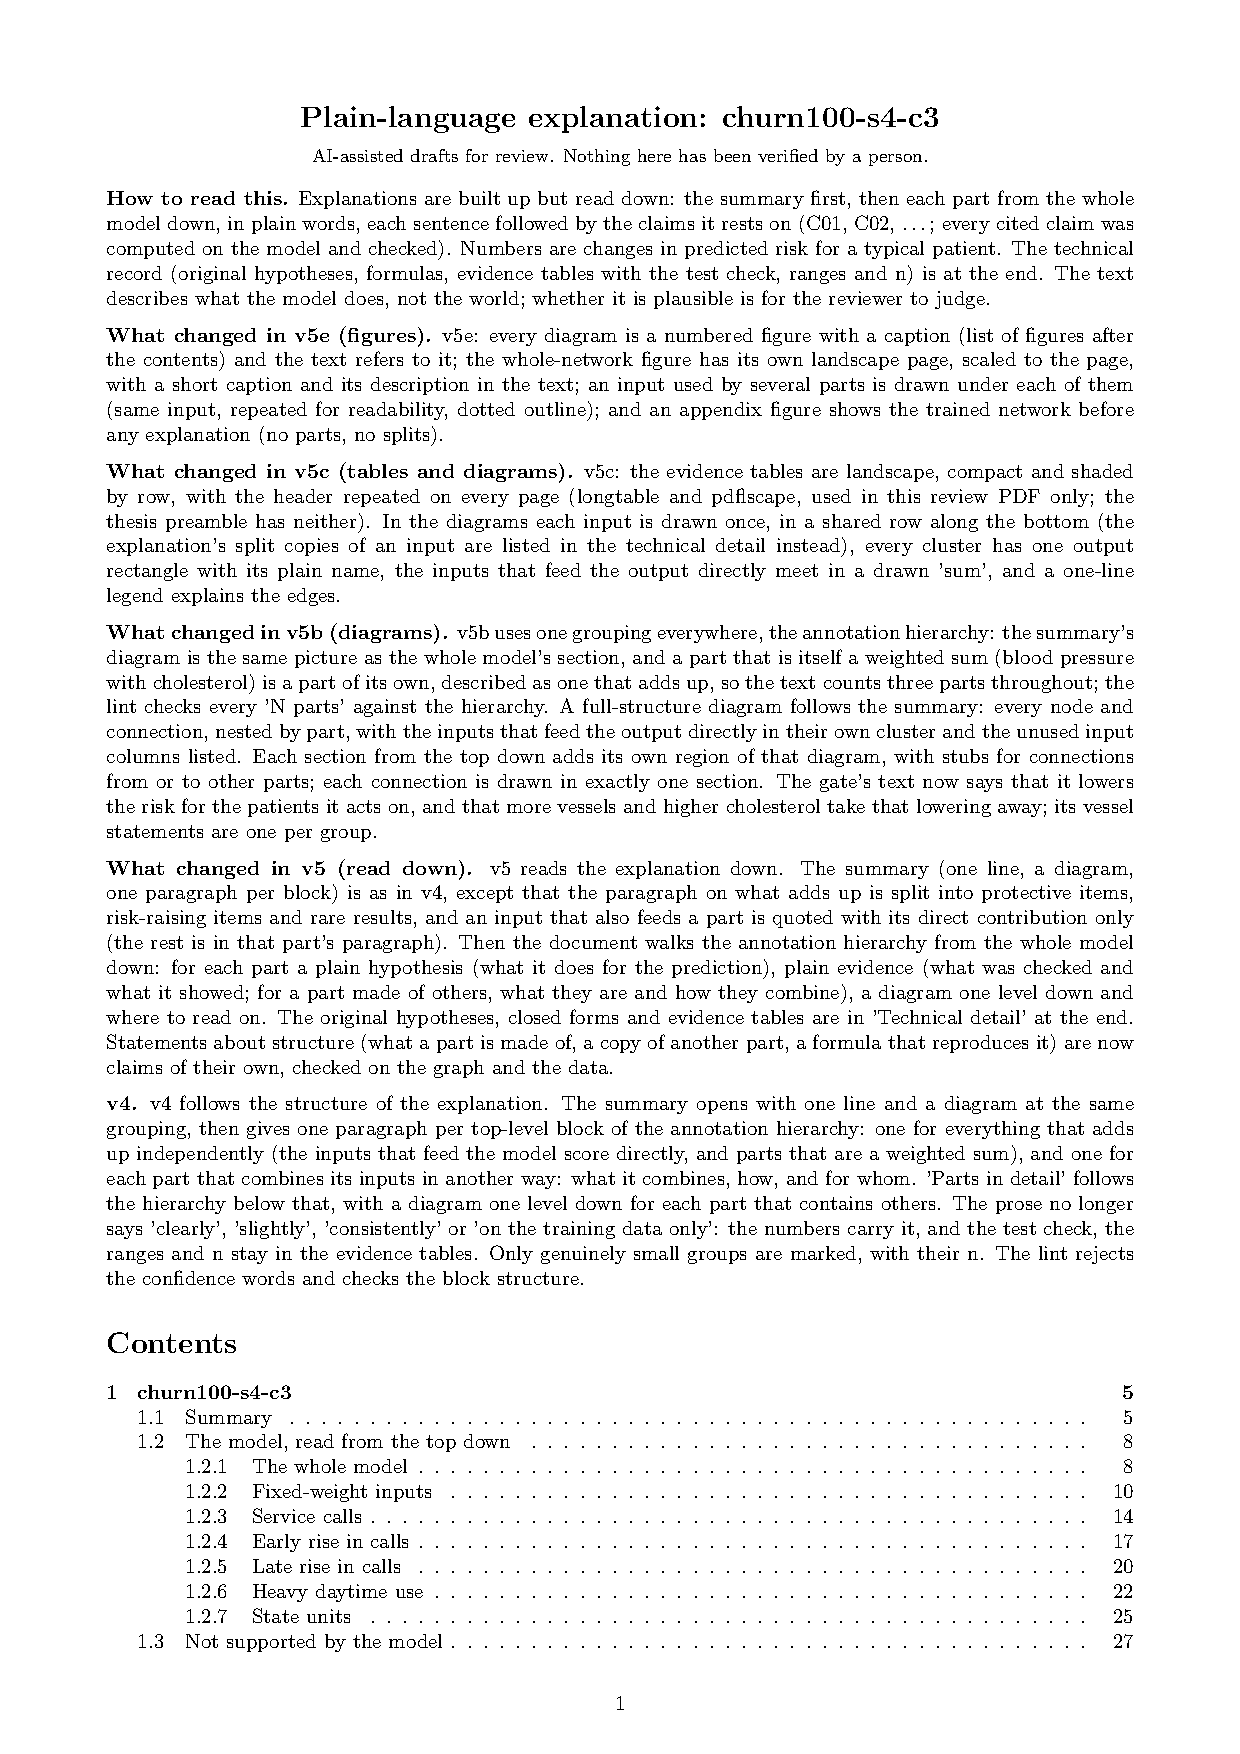
\includepdf[pages={1-6},addtotoc={1,section,1,{churn100-s4-c3: plain-language explanation (read-down document)},plain:churn100-s4-c3}]{churn100-s4-c3/churn100-s4-c3-plain-v5.pdf}
\includepdf[pages={7},landscape]{churn100-s4-c3/churn100-s4-c3-plain-v5.pdf}
\includepdf[pages={8-28}]{churn100-s4-c3/churn100-s4-c3-plain-v5.pdf}
\includepdf[pages={29-34},landscape]{churn100-s4-c3/churn100-s4-c3-plain-v5.pdf}
\includepdf[pages={35}]{churn100-s4-c3/churn100-s4-c3-plain-v5.pdf}
\includepdf[pages={36-39},landscape]{churn100-s4-c3/churn100-s4-c3-plain-v5.pdf}
\includepdf[pages={40}]{churn100-s4-c3/churn100-s4-c3-plain-v5.pdf}
\includepdf[pages={41},landscape]{churn100-s4-c3/churn100-s4-c3-plain-v5.pdf}
\includepdf[pages={42}]{churn100-s4-c3/churn100-s4-c3-plain-v5.pdf}
\includepdf[pages={43},landscape]{churn100-s4-c3/churn100-s4-c3-plain-v5.pdf}
\includepdf[pages={44}]{churn100-s4-c3/churn100-s4-c3-plain-v5.pdf}
\includepdf[pages={45},landscape]{churn100-s4-c3/churn100-s4-c3-plain-v5.pdf}
\includepdf[pages={46}]{churn100-s4-c3/churn100-s4-c3-plain-v5.pdf}
\includepdf[pages={47},landscape]{churn100-s4-c3/churn100-s4-c3-plain-v5.pdf}
\includepdf[pages={48}]{churn100-s4-c3/churn100-s4-c3-plain-v5.pdf}
\includepdf[pages={49-50},landscape]{churn100-s4-c3/churn100-s4-c3-plain-v5.pdf}
\includepdf[pages={51}]{churn100-s4-c3/churn100-s4-c3-plain-v5.pdf}
\includepdf[pages={52},landscape]{churn100-s4-c3/churn100-s4-c3-plain-v5.pdf}
\includepdf[pages={53}]{churn100-s4-c3/churn100-s4-c3-plain-v5.pdf}
\addcontentsline{toc}{section}{churn100-s4-c3: coverage certificate}
% Coverage certificate for churn100-s4-c3 (genome 27f540ac-6acb-4d58-9972-cd71fae31cf0); content sha256 99f3bce0c6f3eff7e465b5d629b8c3ce8fae606cf84601487b0a16525378c202.
\providecommand{\explaneatcertdir}[1]{}
\begin{drafted}[churn100-s4-c3 coverage certificate]
\section{Coverage certificate: churn100-s4-c3}\label{app:churn100-s4-c3:sec}
Provenance, coverage and checks of the explanation, rendered from the canonical JSON record \texttt{churn100-s4-c3.json} (schema 1.4.0, SHA-256 \texttt{99f3bce0c6f3eff7}\ldots). The explanation itself (summary, parts, evidence, figures) is the read-down document before this page.

\begin{table}[htbp]
\centering\small
\begin{tabularx}{\linewidth}{@{}lX@{}}
\toprule
Dataset & churn\_\allowbreak{}onehot \\
Experiment & churn100-s4, seed 4 \\
Genome & \texttt{27f540ac-6acb-4d58-9972-cd71fae31cf0} (NEAT key 24445, generation 99) \\
Explanation & \texttt{ffdb207f-1e0f-4d2e-a330-f47b1ca75c4a} (89 operations) \\
Train AUC / accuracy & 0.8884 / 0.8795 (n = 4000) \\
Test AUC / accuracy & 0.8671 / 0.875 (n = 1000) \\
Output activation & sigmoid \\
Phenotype & 93 nodes (71 inputs, 21 hidden, 1 output), 76 enabled edges \\
Explained model state & 103 nodes, 78 enabled edges \\
Refactoring operations & add\_\allowbreak{}identity\_\allowbreak{}node 2, consolidate\_\allowbreak{}node 1, split\_\allowbreak{}node 8 \\
Function preservation & max $|\Delta\,\mathrm{output}|$ = $4.44\times 10^{-16}$ on the training split \\
Annotations & 7 (5 leaf, 2 composition) \\
Structural coverage & 1 (102 of 102 candidate nodes; 30 Null) \\
Compositional coverage & 1 \\
Uncovered nodes / edges & 0 / 0 \\
Missing compositions & 0 \\
Full coverage & yes \\
Drafted by & AI-assisted draft \\
Verified by & unverified \\
Record hash (SHA-256) & \texttt{99f3bce0c6f3eff7}\ldots \\
\bottomrule
\end{tabularx}
\caption{Explanation certificate summary: churn100-s4-c3.}
\label{app:churn100-s4-c3:summary}
\end{table}
\subsection{Coverage}\label{app:churn100-s4-c3:coverage}
Coverage is computed by the current code (the function behind the \texttt{get\_coverage} tool) under these conventions. \emph{Candidate nodes} are all nodes of the explained model state except the output nodes. A candidate node is \emph{covered} when some annotation of the hierarchy (a leaf, or a composition together with its descendants) contains it and all its enabled outgoing edges. \emph{Exact Null} parts, which have no effect on any output for any input, count as covered: nodes with no path to an output over enabled, non-zero-weight edges (disconnected inputs and dead ends), and edges that have zero weight or touch such a node. Compositional coverage is the fraction of required compositions present: every annotation except a single global root containing every output must have a parent; a parentless, childless annotation made only of Null nodes is exempt.

\begin{itemize}
\item \textbf{Null, disconnected input (30):} \texttt{-10} (state:17), \texttt{-13} (state:2), \texttt{-14} (state:20), \texttt{-16} (state:22), \texttt{-17} (state:23), \texttt{-18} (state:24), \texttt{-2} (state:1), \texttt{-25} (state:30), \texttt{-26} (state:31), \texttt{-27} (state:32), \texttt{-30} (state:35), \texttt{-37} (state:41), \texttt{-39} (state:43), \texttt{-44} (state:48), \texttt{-45} (state:49), \texttt{-47} (state:50), \texttt{-48} (state:6), \texttt{-49} (state:7), \texttt{-5} (state:12), \texttt{-53} (areaCode:408), \texttt{-55} (areaCode:510), \texttt{-6} (state:13), \texttt{-62} (totalEveMinutes), \texttt{-63} (totalEveCalls), \texttt{-65} (totalNightMinutes), \texttt{-66} (totalNightCalls), \texttt{-67} (totalNightCharge), \texttt{-68} (totalIntlMinutes), \texttt{-69} (totalIntlCalls), \texttt{-70} (totalIntlCharge).
\item \textbf{Uncovered nodes:} none.
\item \textbf{Uncovered edges:} none.
\item \textbf{Missing compositions:} none.
\end{itemize}
\noindent\textbf{Agreement with the \texttt{get\_coverage} tool:} yes.

\subsection{Closed-form checks}\label{app:churn100-s4-c3:closedform}
{\small\noindent\begin{tabularx}{\linewidth}{@{}lXrr@{}}
\toprule Tag & Annotation & Closed form vs forward pass & Exact function vs forward pass \\ \midrule
A1 & churn\_\allowbreak{}logit & 0.00303 & $4.44\times 10^{-16}$ \\
A2 & linear\_\allowbreak{}backbone & 0.00552 & $1.78\times 10^{-15}$ \\
A3 & day\_\allowbreak{}usage\_\allowbreak{}hinges & 0.00207 & $4.44\times 10^{-16}$ \\
A4 & state\_\allowbreak{}offsets & 0.0277 & $4.44\times 10^{-16}$ \\
A5 & service\_\allowbreak{}calls & 0.0157 & $8.88\times 10^{-16}$ \\
A6 & csc\_\allowbreak{}late\_\allowbreak{}chain & 0.00148 & $2.22\times 10^{-16}$ \\
A7 & csc\_\allowbreak{}early\_\allowbreak{}hinge & 0.00608 & 0 \\
\bottomrule
\end{tabularx}\par}
\subsection{Refactoring operations}\label{app:churn100-s4-c3:operations}
The explained model state is the phenotype after these operations, replayed in order. All are function-preserving; the largest change in the model output over the 4000 training rows is $4.44\times 10^{-16}$ (tolerance $1.00\times 10^{-9}$).
\begin{itemize}
\item \#71: split \texttt{-71} into \texttt{-71\_\allowbreak{}a}, \texttt{-71\_\allowbreak{}b}, \texttt{-71\_\allowbreak{}c}.
\item \#72: split \texttt{-60} into \texttt{-60\_\allowbreak{}a}, \texttt{-60\_\allowbreak{}b}.
\item \#73: split \texttt{-57} into \texttt{-57\_\allowbreak{}a}, \texttt{-57\_\allowbreak{}b}.
\item \#74: split \texttt{-51} into \texttt{-51\_\allowbreak{}a}, \texttt{-51\_\allowbreak{}b}.
\item \#75: split \texttt{-42} into \texttt{-42\_\allowbreak{}a}, \texttt{-42\_\allowbreak{}b}.
\item \#76: split \texttt{-34} into \texttt{-34\_\allowbreak{}a}, \texttt{-34\_\allowbreak{}b}.
\item \#77: split \texttt{-28} into \texttt{-28\_\allowbreak{}a}, \texttt{-28\_\allowbreak{}b}.
\item \#78: split \texttt{-23} into \texttt{-23\_\allowbreak{}a}, \texttt{-23\_\allowbreak{}b}.
\item \#79: consolidate \texttt{-71\_\allowbreak{}a}, \texttt{-71\_\allowbreak{}c}.
\item \#80: identity node \texttt{identity\_\allowbreak{}lin} before \texttt{0} (28 connection(s)).
\item \#81: identity node \texttt{identity\_\allowbreak{}svc} before \texttt{0} (3 connection(s)).
\end{itemize}
\subsection{Audit against the definitions}\label{app:churn100-s4-c3:audit}
Automatic findings on the stored explanation (codes as in the JSON record's \texttt{issues}); they flag what an examiner should check, not verdicts.
\begin{itemize}
\item \textsc{warning} \texttt{unverified}: No human verification is recorded for this explanation.
\end{itemize}
\end{drafted}

\clearpage
\section*{5. churn100-s7-c1: verification checklist}
\addcontentsline{toc}{section}{5. churn100-s7-c1: verification checklist}
\label{rev:churn100-s7-c1}
\textbf{Already recorded:} nothing (no verdict in the record).

\textbf{Recorded vs live.} Agent = the drafting agent's report; orchestrator = the record's automated re-check; live = this export (current code, training split).

{\footnotesize
\begin{tabularx}{\linewidth}{@{}>{\raggedright\arraybackslash}X>{\raggedright\arraybackslash}p{2.1cm}>{\raggedright\arraybackslash}p{3.0cm}>{\raggedright\arraybackslash}p{3.0cm}l@{}}
\toprule
Check & Agent & Orchestrator & Live & Status \\
\midrule
Function preservation, max $|$change in output$|$ & 1.22e-15 & 1.22e-15 & 1.22e-15 & agree \\
Closed-form max abs error (all leaves) & 0.03806 & 0.03806 & 0.03806 & agree \\
Numeric-function max abs error & n/a & 8.88e-16 & 8.88e-16 & agree \\
Structural coverage & 1 & 1 & 1 & agree \\
Compositional coverage & 1 & 1 & 1 & agree \\
Hierarchy complete & yes & yes & yes & agree \\
Root annotation & n/a & churn\_\allowbreak{}logit & churn\_\allowbreak{}logit & agree \\
Leaf / composition counts & 5 / 2 & n/a & 5 / 2 & agree \\
Operation counts & 5 splits, 2 identity & add identity node 2, annotate 7, rename node 71, split node 5 & add identity node 2, annotate 7, rename node 71, split node 5 & agree \\
Full coverage & yes & yes & yes & agree \\
\bottomrule
\end{tabularx}}

\textbf{What to look at.}
\begin{itemize}
\item Largest closed-form error: \texttt{state\_\allowbreak{}offsets} (0.0381). This is the cost of the 3 s.f. display rounding, in the exit's own units; the numeric function is exact. Check that the rounded formula still supports the hypothesis as worded.
\item Strong claim in \texttt{state\_\allowbreak{}offsets}: \emph{``always active, constant +0.008), 5667 state:2 is never active (dead unit, zero effect).''} Is this (exactness, threshold, rare category) supported by the evidence, or fitted to a few rows?
\item Strong claim in \texttt{intl\_\allowbreak{}plan\_\allowbreak{}switch}: \emph{``linear replacement 0.9189 (identical, exact switch).''} Is this (exactness, threshold, rare category) supported by the evidence, or fitted to a few rows?
\item 5 split(s), all of input nodes (an input feeding two annotations). These are routine; check only that each input copy sits in the annotation whose hypothesis uses it.
\item Read the root's hypothesis against its closed form: does the stated combination of children (additive, gated, serial) match the formula?
\end{itemize}
\textbf{Tool notes (record):} None new. Tool calls driven from scratch Python scripts that run experiments/\allowbreak{}species\_\allowbreak{}leads/\allowbreak{}xn.py per call (all logged), because the worktree-isolated Bash refuses compound shell commands. Ablations at output-term level on the original phenotype (local numpy).

\textbf{Plain-language layer} (AI-assisted draft for review (unverified)): the read-down document follows this page (summary, parts, evidence, worth checking; also \texttt{churn100-s7-c1-plain-v5.pdf} in this genome's folder). Record a verdict on it with \texttt{uv run python -m explaneat export record-plain-verdict churn100-s7-c1 --verified --minutes N --notes "..."}.

\textbf{Verdict.}

\begin{tabularx}{\linewidth}{@{}lX@{}}
Verified (correct as it stands, or after my changes): & $\square$ yes \quad $\square$ no \\[4pt]
Minutes: & \rule{3cm}{0.4pt} \\[4pt]
Changes: & \rule{\linewidth}{0.4pt} \\[10pt]
 & \rule{\linewidth}{0.4pt} \\[4pt]
Notes: & \rule{\linewidth}{0.4pt} \\[10pt]
 & \rule{\linewidth}{0.4pt} \\
\end{tabularx}

\textbf{Record it} (writes \texttt{mike\_verification} into \texttt{experiments/10seed/explanations/churn100-s7-c1.json}; use \texttt{-{}-not-verified} for no; rebuild the CSVs with \texttt{uv run python experiments/10seed/build\_explanations\_csv.py}):

{\footnotesize\raggedright\texttt{uv run python -m explaneat export record-verdict churn100-s7-c1 --verified --minutes N --changes "..." --notes "..."}\par}


\clearpage
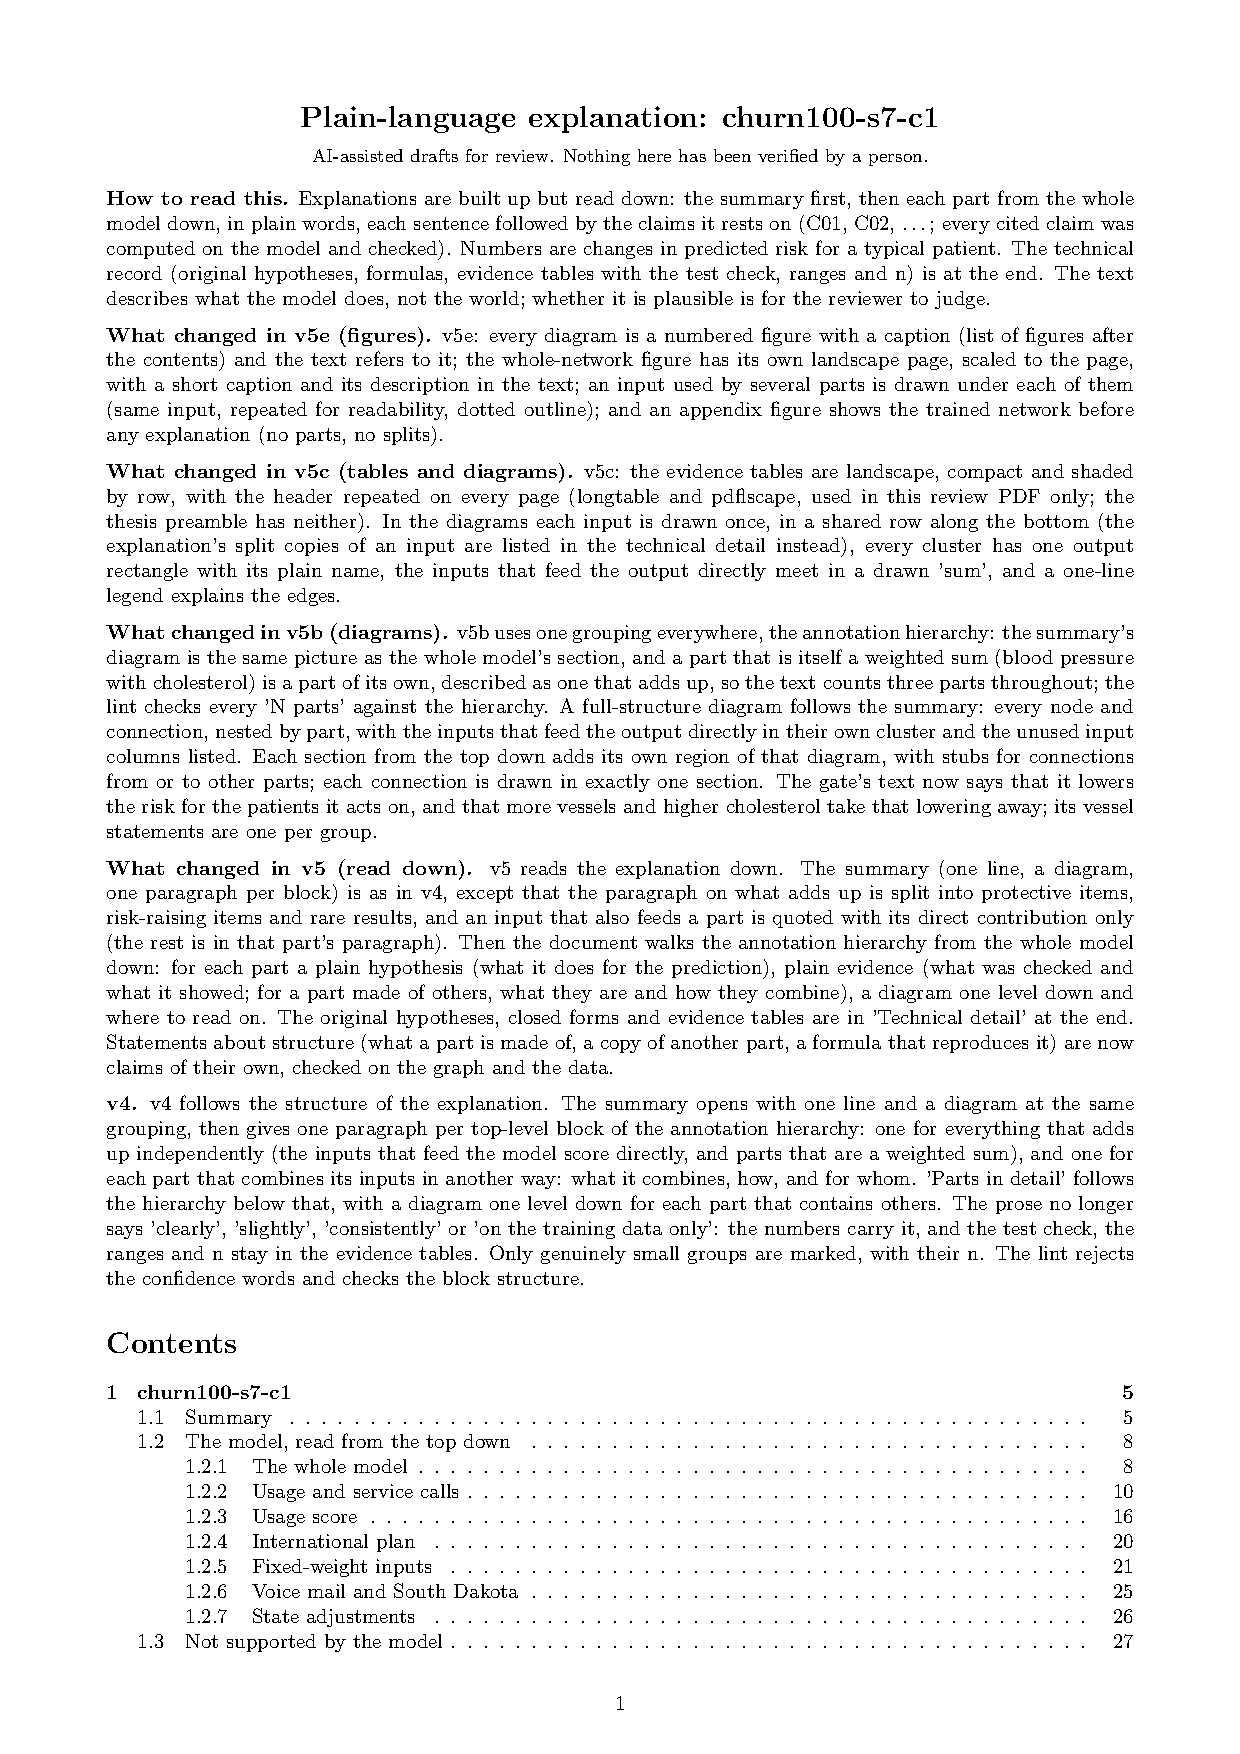
\includepdf[pages={1-6},addtotoc={1,section,1,{churn100-s7-c1: plain-language explanation (read-down document)},plain:churn100-s7-c1}]{churn100-s7-c1/churn100-s7-c1-plain-v5.pdf}
\includepdf[pages={7},landscape]{churn100-s7-c1/churn100-s7-c1-plain-v5.pdf}
\includepdf[pages={8-29}]{churn100-s7-c1/churn100-s7-c1-plain-v5.pdf}
\includepdf[pages={30-32},landscape]{churn100-s7-c1/churn100-s7-c1-plain-v5.pdf}
\includepdf[pages={33}]{churn100-s7-c1/churn100-s7-c1-plain-v5.pdf}
\includepdf[pages={34},landscape]{churn100-s7-c1/churn100-s7-c1-plain-v5.pdf}
\includepdf[pages={35}]{churn100-s7-c1/churn100-s7-c1-plain-v5.pdf}
\includepdf[pages={36-37},landscape]{churn100-s7-c1/churn100-s7-c1-plain-v5.pdf}
\includepdf[pages={38}]{churn100-s7-c1/churn100-s7-c1-plain-v5.pdf}
\includepdf[pages={39},landscape]{churn100-s7-c1/churn100-s7-c1-plain-v5.pdf}
\includepdf[pages={40}]{churn100-s7-c1/churn100-s7-c1-plain-v5.pdf}
\includepdf[pages={41-43},landscape]{churn100-s7-c1/churn100-s7-c1-plain-v5.pdf}
\includepdf[pages={44}]{churn100-s7-c1/churn100-s7-c1-plain-v5.pdf}
\includepdf[pages={45},landscape]{churn100-s7-c1/churn100-s7-c1-plain-v5.pdf}
\includepdf[pages={46}]{churn100-s7-c1/churn100-s7-c1-plain-v5.pdf}
\includepdf[pages={47},landscape]{churn100-s7-c1/churn100-s7-c1-plain-v5.pdf}
\includepdf[pages={48}]{churn100-s7-c1/churn100-s7-c1-plain-v5.pdf}
\includepdf[pages={49},landscape]{churn100-s7-c1/churn100-s7-c1-plain-v5.pdf}
\includepdf[pages={50}]{churn100-s7-c1/churn100-s7-c1-plain-v5.pdf}
\addcontentsline{toc}{section}{churn100-s7-c1: coverage certificate}
% Coverage certificate for churn100-s7-c1 (genome 32d24e98-266e-450c-88c8-5bdc1abbf5dd); content sha256 55f21bd4a4575c9cef1911b86f7cdc477cd27f4f9f1fd04622ee2dc885b3c9fe.
\providecommand{\explaneatcertdir}[1]{}
\begin{drafted}[churn100-s7-c1 coverage certificate]
\section{Coverage certificate: churn100-s7-c1}\label{app:churn100-s7-c1:sec}
Provenance, coverage and checks of the explanation, rendered from the canonical JSON record \texttt{churn100-s7-c1.json} (schema 1.4.0, SHA-256 \texttt{55f21bd4a4575c9c}\ldots). The explanation itself (summary, parts, evidence, figures) is the read-down document before this page.

\begin{table}[htbp]
\centering\small
\begin{tabularx}{\linewidth}{@{}lX@{}}
\toprule
Dataset & churn\_\allowbreak{}onehot \\
Experiment & churn100-s7, seed 7 \\
Genome & \texttt{32d24e98-266e-450c-88c8-5bdc1abbf5dd} (NEAT key 20708, generation 99) \\
Explanation & \texttt{b370983e-3d7d-40c8-8b8f-f37c41a96cc1} (85 operations) \\
Train AUC / accuracy & 0.9189 / 0.921 (n = 4000) \\
Test AUC / accuracy & 0.9007 / 0.921 (n = 1000) \\
Output activation & sigmoid \\
Phenotype & 86 nodes (71 inputs, 14 hidden, 1 output), 59 enabled edges \\
Explained model state & 95 nodes, 61 enabled edges \\
Refactoring operations & add\_\allowbreak{}identity\_\allowbreak{}node 2, split\_\allowbreak{}node 5 \\
Function preservation & max $|\Delta\,\mathrm{output}|$ = $1.22\times 10^{-15}$ on the training split \\
Annotations & 7 (5 leaf, 2 composition) \\
Structural coverage & 1 (94 of 94 candidate nodes; 35 Null) \\
Compositional coverage & 1 \\
Uncovered nodes / edges & 0 / 0 \\
Missing compositions & 0 \\
Full coverage & yes \\
Drafted by & AI-assisted draft \\
Verified by & unverified \\
Record hash (SHA-256) & \texttt{55f21bd4a4575c9c}\ldots \\
\bottomrule
\end{tabularx}
\caption{Explanation certificate summary: churn100-s7-c1.}
\label{app:churn100-s7-c1:summary}
\end{table}
\subsection{Coverage}\label{app:churn100-s7-c1:coverage}
Coverage is computed by the current code (the function behind the \texttt{get\_coverage} tool) under these conventions. \emph{Candidate nodes} are all nodes of the explained model state except the output nodes. A candidate node is \emph{covered} when some annotation of the hierarchy (a leaf, or a composition together with its descendants) contains it and all its enabled outgoing edges. \emph{Exact Null} parts, which have no effect on any output for any input, count as covered: nodes with no path to an output over enabled, non-zero-weight edges (disconnected inputs and dead ends), and edges that have zero weight or touch such a node. Compositional coverage is the fraction of required compositions present: every annotation except a single global root containing every output must have a parent; a parentless, childless annotation made only of Null nodes is exempt.

\begin{itemize}
\item \textbf{Null, disconnected input (35):} \texttt{-11} (state:18), \texttt{-12} (state:19), \texttt{-15} (state:21), \texttt{-16} (state:22), \texttt{-17} (state:23), \texttt{-18} (state:24), \texttt{-2} (state:1), \texttt{-23} (state:29), \texttt{-24} (state:3), \texttt{-25} (state:30), \texttt{-28} (state:33), \texttt{-29} (state:34), \texttt{-31} (state:36), \texttt{-33} (state:38), \texttt{-35} (state:4), \texttt{-38} (state:42), \texttt{-39} (state:43), \texttt{-4} (state:11), \texttt{-40} (state:44), \texttt{-47} (state:50), \texttt{-48} (state:6), \texttt{-49} (state:7), \texttt{-5} (state:12), \texttt{-50} (state:8), \texttt{-51} (state:9), \texttt{-53} (areaCode:408), \texttt{-54} (areaCode:415), \texttt{-6} (state:13), \texttt{-60} (totalDayCalls), \texttt{-63} (totalEveCalls), \texttt{-64} (totalEveCharge), \texttt{-67} (totalNightCharge), \texttt{-68} (totalIntlMinutes), \texttt{-7} (state:14), \texttt{-9} (state:16).
\item \textbf{Uncovered nodes:} none.
\item \textbf{Uncovered edges:} none.
\item \textbf{Missing compositions:} none.
\end{itemize}
\noindent\textbf{Agreement with the \texttt{get\_coverage} tool:} yes.

\subsection{Closed-form checks}\label{app:churn100-s7-c1:closedform}
{\small\noindent\begin{tabularx}{\linewidth}{@{}lXrr@{}}
\toprule Tag & Annotation & Closed form vs forward pass & Exact function vs forward pass \\ \midrule
A1 & churn\_\allowbreak{}logit & 0.00775 & $7.77\times 10^{-16}$ \\
A2 & linear\_\allowbreak{}backbone & 0.00352 & $8.88\times 10^{-16}$ \\
A3 & vmail\_\allowbreak{}state41\_\allowbreak{}unit & 0.00187 & 0 \\
A4 & intl\_\allowbreak{}plan\_\allowbreak{}switch & 0.00131 & 0 \\
A5 & state\_\allowbreak{}offsets & 0.0381 & 0 \\
A6 & usage\_\allowbreak{}response & 0.0254 & $4.44\times 10^{-15}$ \\
A7 & usage\_\allowbreak{}hinge & 0.00297 & $4.44\times 10^{-16}$ \\
\bottomrule
\end{tabularx}\par}
\subsection{Refactoring operations}\label{app:churn100-s7-c1:operations}
The explained model state is the phenotype after these operations, replayed in order. All are function-preserving; the largest change in the model output over the 4000 training rows is $1.22\times 10^{-15}$ (tolerance $1.00\times 10^{-9}$).
\begin{itemize}
\item \#71: split \texttt{-37} into \texttt{-37\_\allowbreak{}a}, \texttt{-37\_\allowbreak{}b}, \texttt{-37\_\allowbreak{}c}, \texttt{-37\_\allowbreak{}d}.
\item \#72: split \texttt{-57} into \texttt{-57\_\allowbreak{}a}, \texttt{-57\_\allowbreak{}b}.
\item \#73: split \texttt{-62} into \texttt{-62\_\allowbreak{}a}, \texttt{-62\_\allowbreak{}b}.
\item \#74: split \texttt{-65} into \texttt{-65\_\allowbreak{}a}, \texttt{-65\_\allowbreak{}b}.
\item \#75: split \texttt{-41} into \texttt{-41\_\allowbreak{}a}, \texttt{-41\_\allowbreak{}b}.
\item \#76: identity node \texttt{identity\_\allowbreak{}lin} before \texttt{0} (27 connection(s)).
\item \#77: identity node \texttt{identity\_\allowbreak{}usage} before \texttt{0} (3 connection(s)).
\end{itemize}
\subsection{Audit against the definitions}\label{app:churn100-s7-c1:audit}
Automatic findings on the stored explanation (codes as in the JSON record's \texttt{issues}); they flag what an examiner should check, not verdicts.
\begin{itemize}
\item \textsc{warning} \texttt{unverified}: No human verification is recorded for this explanation.
\end{itemize}
\end{drafted}

\clearpage
\section*{6. heart-s1-c1: verification checklist}
\addcontentsline{toc}{section}{6. heart-s1-c1: verification checklist}
\label{rev:heart-s1-c1}
\textbf{Already recorded:} nothing (no verdict in the record).

\textbf{Recorded vs live.} Agent = the drafting agent's report; orchestrator = the record's automated re-check; live = this export (current code, training split).

{\footnotesize
\begin{tabularx}{\linewidth}{@{}>{\raggedright\arraybackslash}X>{\raggedright\arraybackslash}p{2.1cm}>{\raggedright\arraybackslash}p{3.0cm}>{\raggedright\arraybackslash}p{3.0cm}l@{}}
\toprule
Check & Agent & Orchestrator & Live & Status \\
\midrule
Function preservation, max $|$change in output$|$ & 3.33e-16 & 3.33e-16 & 3.33e-16 & agree \\
Closed-form max abs error (all leaves) & 0.00514 & 0.00514 & 0.00514 & agree \\
Numeric-function max abs error & n/a & 0 & 0 & agree \\
Structural coverage & 1 & 1 & 1 & agree \\
Compositional coverage & 1 & 1 & 1 & agree \\
Hierarchy complete & yes & yes & yes & agree \\
Root annotation & n/a & heart\_\allowbreak{}disease\_\allowbreak{}logit & heart\_\allowbreak{}disease\_\allowbreak{}logit & agree \\
Leaf / composition counts & 5 / 1 & n/a & 5 / 1 & agree \\
Operation counts & 3 splits, 0 identity & annotate 6, rename node 26, split node 3 & annotate 6, rename node 26, split node 3 & agree \\
Full coverage & yes & yes & yes & agree \\
\bottomrule
\end{tabularx}}

\textbf{What to look at.}
\begin{itemize}
\item Largest closed-form error: \texttt{st\_\allowbreak{}depression\_\allowbreak{}normal\_\allowbreak{}ecg\_\allowbreak{}gate} (0.00514). This is the cost of the 3 s.f. display rounding, in the exit's own units; the numeric function is exact. Check that the rounded formula still supports the hypothesis as worded.
\item Strong claim in \texttt{ca\_\allowbreak{}slope2\_\allowbreak{}relay}: \emph{``Evidence (train, n=242): pre-activation 0.28..2.19, never clips, so the part is exactly affine on the data;''} Is this (exactness, threshold, rare category) supported by the evidence, or fitted to a few rows?
\item Strong claim in \texttt{st\_\allowbreak{}depression\_\allowbreak{}normal\_\allowbreak{}ecg\_\allowbreak{}gate}: \emph{``Hypothesis: node 1801 = ReLU(1.542 restecg:0 + 0.817 oldpeak - 1.521) is a gate in which ST depression (oldpeak) raises predicted risk only for patients with a normal resting ECG (restecg:0), once oldpeak is above about its mean (...''} Is this (exactness, threshold, rare category) supported by the evidence, or fitted to a few rows?
\item 3 split(s), all of input nodes (an input feeding two annotations). These are routine; check only that each input copy sits in the annotation whose hypothesis uses it.
\item Read the root's hypothesis against its closed form: does the stated combination of children (additive, gated, serial) match the formula?
\end{itemize}
\textbf{Tool notes (record):} Root annotation via apply\_\allowbreak{}operation must exclude child subgraph nodes (passing the whole graph is refused as 'already covered'); not a bug, but undocumented in the protocol. Otherwise none observed with v3 tooling.

\textbf{Plain-language layer} (AI-assisted draft for review (unverified)): the read-down document follows this page (summary, parts, evidence, worth checking; also \texttt{heart-s1-c1-plain-v5.pdf} in this genome's folder). Record a verdict on it with \texttt{uv run python -m explaneat export record-plain-verdict heart-s1-c1 --verified --minutes N --notes "..."}.

\textbf{Verdict.}

\begin{tabularx}{\linewidth}{@{}lX@{}}
Verified (correct as it stands, or after my changes): & $\square$ yes \quad $\square$ no \\[4pt]
Minutes: & \rule{3cm}{0.4pt} \\[4pt]
Changes: & \rule{\linewidth}{0.4pt} \\[10pt]
 & \rule{\linewidth}{0.4pt} \\[4pt]
Notes: & \rule{\linewidth}{0.4pt} \\[10pt]
 & \rule{\linewidth}{0.4pt} \\
\end{tabularx}

\textbf{Record it} (writes \texttt{mike\_verification} into \texttt{experiments/10seed/explanations/heart-s1-c1.json}; use \texttt{-{}-not-verified} for no; rebuild the CSVs with \texttt{uv run python experiments/10seed/build\_explanations\_csv.py}):

{\footnotesize\raggedright\texttt{uv run python -m explaneat export record-verdict heart-s1-c1 --verified --minutes N --changes "..." --notes "..."}\par}


\clearpage
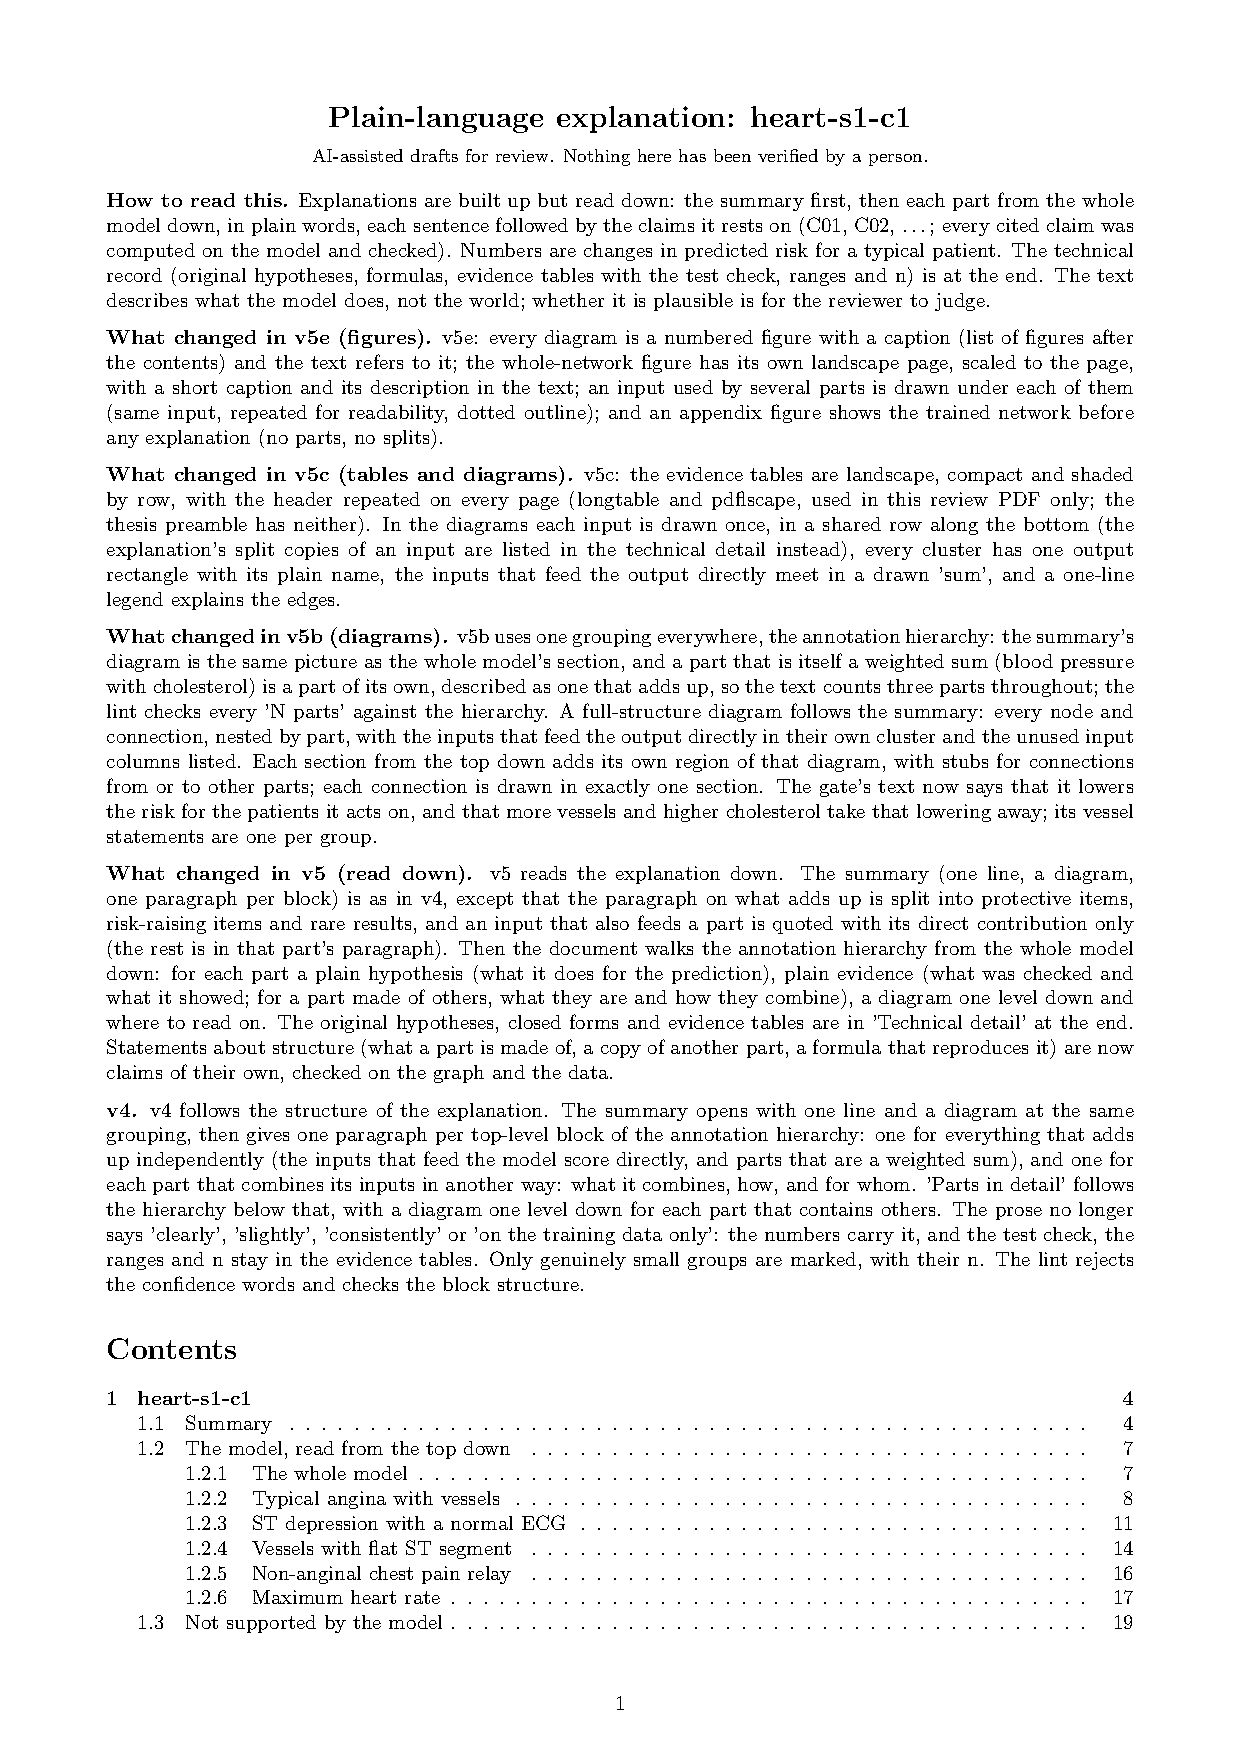
\includepdf[pages={1-5},addtotoc={1,section,1,{heart-s1-c1: plain-language explanation (read-down document)},plain:heart-s1-c1}]{heart-s1-c1/heart-s1-c1-plain-v5.pdf}
\includepdf[pages={6},landscape]{heart-s1-c1/heart-s1-c1-plain-v5.pdf}
\includepdf[pages={7-20}]{heart-s1-c1/heart-s1-c1-plain-v5.pdf}
\includepdf[pages={21-23},landscape]{heart-s1-c1/heart-s1-c1-plain-v5.pdf}
\includepdf[pages={24}]{heart-s1-c1/heart-s1-c1-plain-v5.pdf}
\includepdf[pages={25},landscape]{heart-s1-c1/heart-s1-c1-plain-v5.pdf}
\includepdf[pages={26}]{heart-s1-c1/heart-s1-c1-plain-v5.pdf}
\includepdf[pages={27},landscape]{heart-s1-c1/heart-s1-c1-plain-v5.pdf}
\includepdf[pages={28}]{heart-s1-c1/heart-s1-c1-plain-v5.pdf}
\includepdf[pages={29},landscape]{heart-s1-c1/heart-s1-c1-plain-v5.pdf}
\includepdf[pages={30}]{heart-s1-c1/heart-s1-c1-plain-v5.pdf}
\includepdf[pages={31},landscape]{heart-s1-c1/heart-s1-c1-plain-v5.pdf}
\includepdf[pages={32}]{heart-s1-c1/heart-s1-c1-plain-v5.pdf}
\includepdf[pages={33},landscape]{heart-s1-c1/heart-s1-c1-plain-v5.pdf}
\includepdf[pages={34}]{heart-s1-c1/heart-s1-c1-plain-v5.pdf}
\includepdf[pages={35},landscape]{heart-s1-c1/heart-s1-c1-plain-v5.pdf}
\includepdf[pages={36}]{heart-s1-c1/heart-s1-c1-plain-v5.pdf}
\addcontentsline{toc}{section}{heart-s1-c1: coverage certificate}
% Coverage certificate for heart-s1-c1 (genome a2df22ce-983d-47b6-bbd6-3176d38ed5ff); content sha256 555774df08fc19cc0dd5fe846e6c3e4fb3823536efda28def15a994d5545f6e2.
\providecommand{\explaneatcertdir}[1]{}
\begin{drafted}[heart-s1-c1 coverage certificate]
\section{Coverage certificate: heart-s1-c1}\label{app:heart-s1-c1:sec}
Provenance, coverage and checks of the explanation, rendered from the canonical JSON record \texttt{heart-s1-c1.json} (schema 1.4.0, SHA-256 \texttt{555774df08fc19cc}\ldots). The explanation itself (summary, parts, evidence, figures) is the read-down document before this page.

\begin{table}[htbp]
\centering\small
\begin{tabularx}{\linewidth}{@{}lX@{}}
\toprule
Dataset & Heart Disease (binary, prepared) \\
Experiment & 10seed-heart-s1, seed 1 \\
Genome & \texttt{a2df22ce-983d-47b6-bbd6-3176d38ed5ff} (NEAT key 9674, generation 39) \\
Explanation & \texttt{492866e6-a73b-4465-92a8-ecad82a2adcc} (35 operations) \\
Train AUC / accuracy & 0.9392 / 0.8802 (n = 242) \\
Test AUC / accuracy & 0.861 / 0.7705 (n = 61) \\
Output activation & sigmoid \\
Phenotype & 34 nodes (26 inputs, 7 hidden, 1 output), 30 enabled edges \\
Explained model state & 38 nodes, 30 enabled edges \\
Refactoring operations & split\_\allowbreak{}node 3 \\
Function preservation & max $|\Delta\,\mathrm{output}|$ = $3.33\times 10^{-16}$ on the training split \\
Annotations & 6 (5 leaf, 1 composition) \\
Structural coverage & 1 (37 of 37 candidate nodes; 9 Null) \\
Compositional coverage & 1 \\
Uncovered nodes / edges & 0 / 0 \\
Missing compositions & 0 \\
Full coverage & yes \\
Drafted by & AI-assisted draft \\
Verified by & unverified \\
Record hash (SHA-256) & \texttt{555774df08fc19cc}\ldots \\
\bottomrule
\end{tabularx}
\caption{Explanation certificate summary: heart-s1-c1.}
\label{app:heart-s1-c1:summary}
\end{table}
\subsection{Coverage}\label{app:heart-s1-c1:coverage}
Coverage is computed by the current code (the function behind the \texttt{get\_coverage} tool) under these conventions. \emph{Candidate nodes} are all nodes of the explained model state except the output nodes. A candidate node is \emph{covered} when some annotation of the hierarchy (a leaf, or a composition together with its descendants) contains it and all its enabled outgoing edges. \emph{Exact Null} parts, which have no effect on any output for any input, count as covered: nodes with no path to an output over enabled, non-zero-weight edges (disconnected inputs and dead ends), and edges that have zero weight or touch such a node. Compositional coverage is the fraction of required compositions present: every annotation except a single global root containing every output must have a parent; a parentless, childless annotation made only of Null nodes is exempt.

\begin{itemize}
\item \textbf{Null, disconnected input (9):} \texttt{-10} (fbs:0), \texttt{-13} (restecg:1), \texttt{-14} (restecg:2), \texttt{-16} (exang:0), \texttt{-17} (exang:1), \texttt{-19} (slope:1), \texttt{-24} (thal:4), \texttt{-26} (thal:7), \texttt{-3} (sex:1).
\item \textbf{Uncovered nodes:} none.
\item \textbf{Uncovered edges:} none.
\item \textbf{Missing compositions:} none.
\end{itemize}
\noindent\textbf{Agreement with the \texttt{get\_coverage} tool:} yes.

\subsection{Closed-form checks}\label{app:heart-s1-c1:closedform}
{\small\noindent\begin{tabularx}{\linewidth}{@{}lXrr@{}}
\toprule Tag & Annotation & Closed form vs forward pass & Exact function vs forward pass \\ \midrule
A1 & heart\_\allowbreak{}disease\_\allowbreak{}logit & 0.00427 & $4.44\times 10^{-16}$ \\
A2 & ca\_\allowbreak{}slope2\_\allowbreak{}relay & $4.47\times 10^{-4}$ & 0 \\
A3 & cp3\_\allowbreak{}relay & 0.00246 & 0 \\
A4 & st\_\allowbreak{}depression\_\allowbreak{}normal\_\allowbreak{}ecg\_\allowbreak{}gate & 0.00514 & 0 \\
A5 & max\_\allowbreak{}heart\_\allowbreak{}rate\_\allowbreak{}hinge & $7.41\times 10^{-4}$ & 0 \\
A6 & typical\_\allowbreak{}angina\_\allowbreak{}ca\_\allowbreak{}switch & 0.00423 & 0 \\
\bottomrule
\end{tabularx}\par}
\subsection{Refactoring operations}\label{app:heart-s1-c1:operations}
The explained model state is the phenotype after these operations, replayed in order. All are function-preserving; the largest change in the model output over the 242 training rows is $3.33\times 10^{-16}$ (tolerance $1.00\times 10^{-9}$).
\begin{itemize}
\item \#26: split \texttt{-22} into \texttt{-22\_\allowbreak{}a}, \texttt{-22\_\allowbreak{}b}, \texttt{-22\_\allowbreak{}c}.
\item \#27: split \texttt{-20} into \texttt{-20\_\allowbreak{}a}, \texttt{-20\_\allowbreak{}b}.
\item \#28: split \texttt{-15} into \texttt{-15\_\allowbreak{}a}, \texttt{-15\_\allowbreak{}b}.
\end{itemize}
\subsection{Audit against the definitions}\label{app:heart-s1-c1:audit}
Automatic findings on the stored explanation (codes as in the JSON record's \texttt{issues}); they flag what an examiner should check, not verdicts.
\begin{itemize}
\item \textsc{warning} \texttt{unverified}: No human verification is recorded for this explanation.
\end{itemize}
\end{drafted}

\clearpage
\section*{7. heart-s2-c1: verification checklist}
\addcontentsline{toc}{section}{7. heart-s2-c1: verification checklist}
\label{rev:heart-s2-c1}
\textbf{Already recorded:} nothing (no verdict in the record).

\textbf{Recorded vs live.} Agent = the drafting agent's report; orchestrator = the record's automated re-check; live = this export (current code, training split).

{\footnotesize
\begin{tabularx}{\linewidth}{@{}>{\raggedright\arraybackslash}X>{\raggedright\arraybackslash}p{2.1cm}>{\raggedright\arraybackslash}p{3.0cm}>{\raggedright\arraybackslash}p{3.0cm}l@{}}
\toprule
Check & Agent & Orchestrator & Live & Status \\
\midrule
Function preservation, max $|$change in output$|$ & 2.22e-16 & 2.22e-16 & 2.22e-16 & agree \\
Closed-form max abs error (all leaves) & 0.01311 & 0.01311 & 0.01311 & agree \\
Numeric-function max abs error & n/a & 8.88e-16 & 8.88e-16 & agree \\
Structural coverage & 1 & 1 & 1 & agree \\
Compositional coverage & 1 & 1 & 1 & agree \\
Hierarchy complete & yes & yes & yes & agree \\
Root annotation & n/a & heart\_\allowbreak{}disease\_\allowbreak{}logit & heart\_\allowbreak{}disease\_\allowbreak{}logit & agree \\
Leaf / composition counts & 3 / 1 & n/a & 3 / 1 & agree \\
Operation counts & 5 splits, 0 identity & annotate 4, rename node 26, split node 5 & annotate 4, rename node 26, split node 5 & agree \\
Full coverage & yes & yes & yes & agree \\
\bottomrule
\end{tabularx}}

\textbf{What to look at.}
\begin{itemize}
\item Largest closed-form error: \texttt{oldpeak\_\allowbreak{}hinges} (0.0131), then \texttt{age\_\allowbreak{}hr\_\allowbreak{}reserve\_\allowbreak{}gate} (0.0114). This is the cost of the 3 s.f. display rounding, in the exit's own units; the numeric function is exact. Check that the rounded formula still supports the hypothesis as worded.
\item Strong claim in \texttt{age\_\allowbreak{}hr\_\allowbreak{}reserve\_\allowbreak{}gate}: \emph{``Hypothesis: R3195 is an always-on affine relay of thal:7, so the gate is a single ReLU, 1718 = ReLU(-1.524 - 1.502*age + 1.023*thalach - 1.561*thal:7), that opens when the achieved max heart rate is high for the patient's age and...''} Is this (exactness, threshold, rare category) supported by the evidence, or fitted to a few rows?
\item Strong claim in \texttt{oldpeak\_\allowbreak{}hinges}: \emph{``it acts only here and in the flat-slope gate.''} Is this (exactness, threshold, rare category) supported by the evidence, or fitted to a few rows?
\item 5 split(s), all of input nodes (an input feeding two annotations). These are routine; check only that each input copy sits in the annotation whose hypothesis uses it.
\item Read the root's hypothesis against its closed form: does the stated combination of children (additive, gated, serial) match the formula?
\end{itemize}
\textbf{Tool notes (record):} No v3 tool bugs met. compute\_\allowbreak{}shap on all 242 train rows took about a minute. Input fan-out splits (-26, -15, -9, -20, -18) taken from the topology. The agent sandbox refused shell loops calling uv with variables, so tools were called through a small Python subprocess wrapper in scratch (same xn.py).

\textbf{Plain-language layer} (AI-assisted draft for review (unverified)): the read-down document follows this page (summary, parts, evidence, worth checking; also \texttt{heart-s2-c1-plain-v5.pdf} in this genome's folder). Record a verdict on it with \texttt{uv run python -m explaneat export record-plain-verdict heart-s2-c1 --verified --minutes N --notes "..."}.

\textbf{Verdict.}

\begin{tabularx}{\linewidth}{@{}lX@{}}
Verified (correct as it stands, or after my changes): & $\square$ yes \quad $\square$ no \\[4pt]
Minutes: & \rule{3cm}{0.4pt} \\[4pt]
Changes: & \rule{\linewidth}{0.4pt} \\[10pt]
 & \rule{\linewidth}{0.4pt} \\[4pt]
Notes: & \rule{\linewidth}{0.4pt} \\[10pt]
 & \rule{\linewidth}{0.4pt} \\
\end{tabularx}

\textbf{Record it} (writes \texttt{mike\_verification} into \texttt{experiments/10seed/explanations/heart-s2-c1.json}; use \texttt{-{}-not-verified} for no; rebuild the CSVs with \texttt{uv run python experiments/10seed/build\_explanations\_csv.py}):

{\footnotesize\raggedright\texttt{uv run python -m explaneat export record-verdict heart-s2-c1 --verified --minutes N --changes "..." --notes "..."}\par}


\clearpage
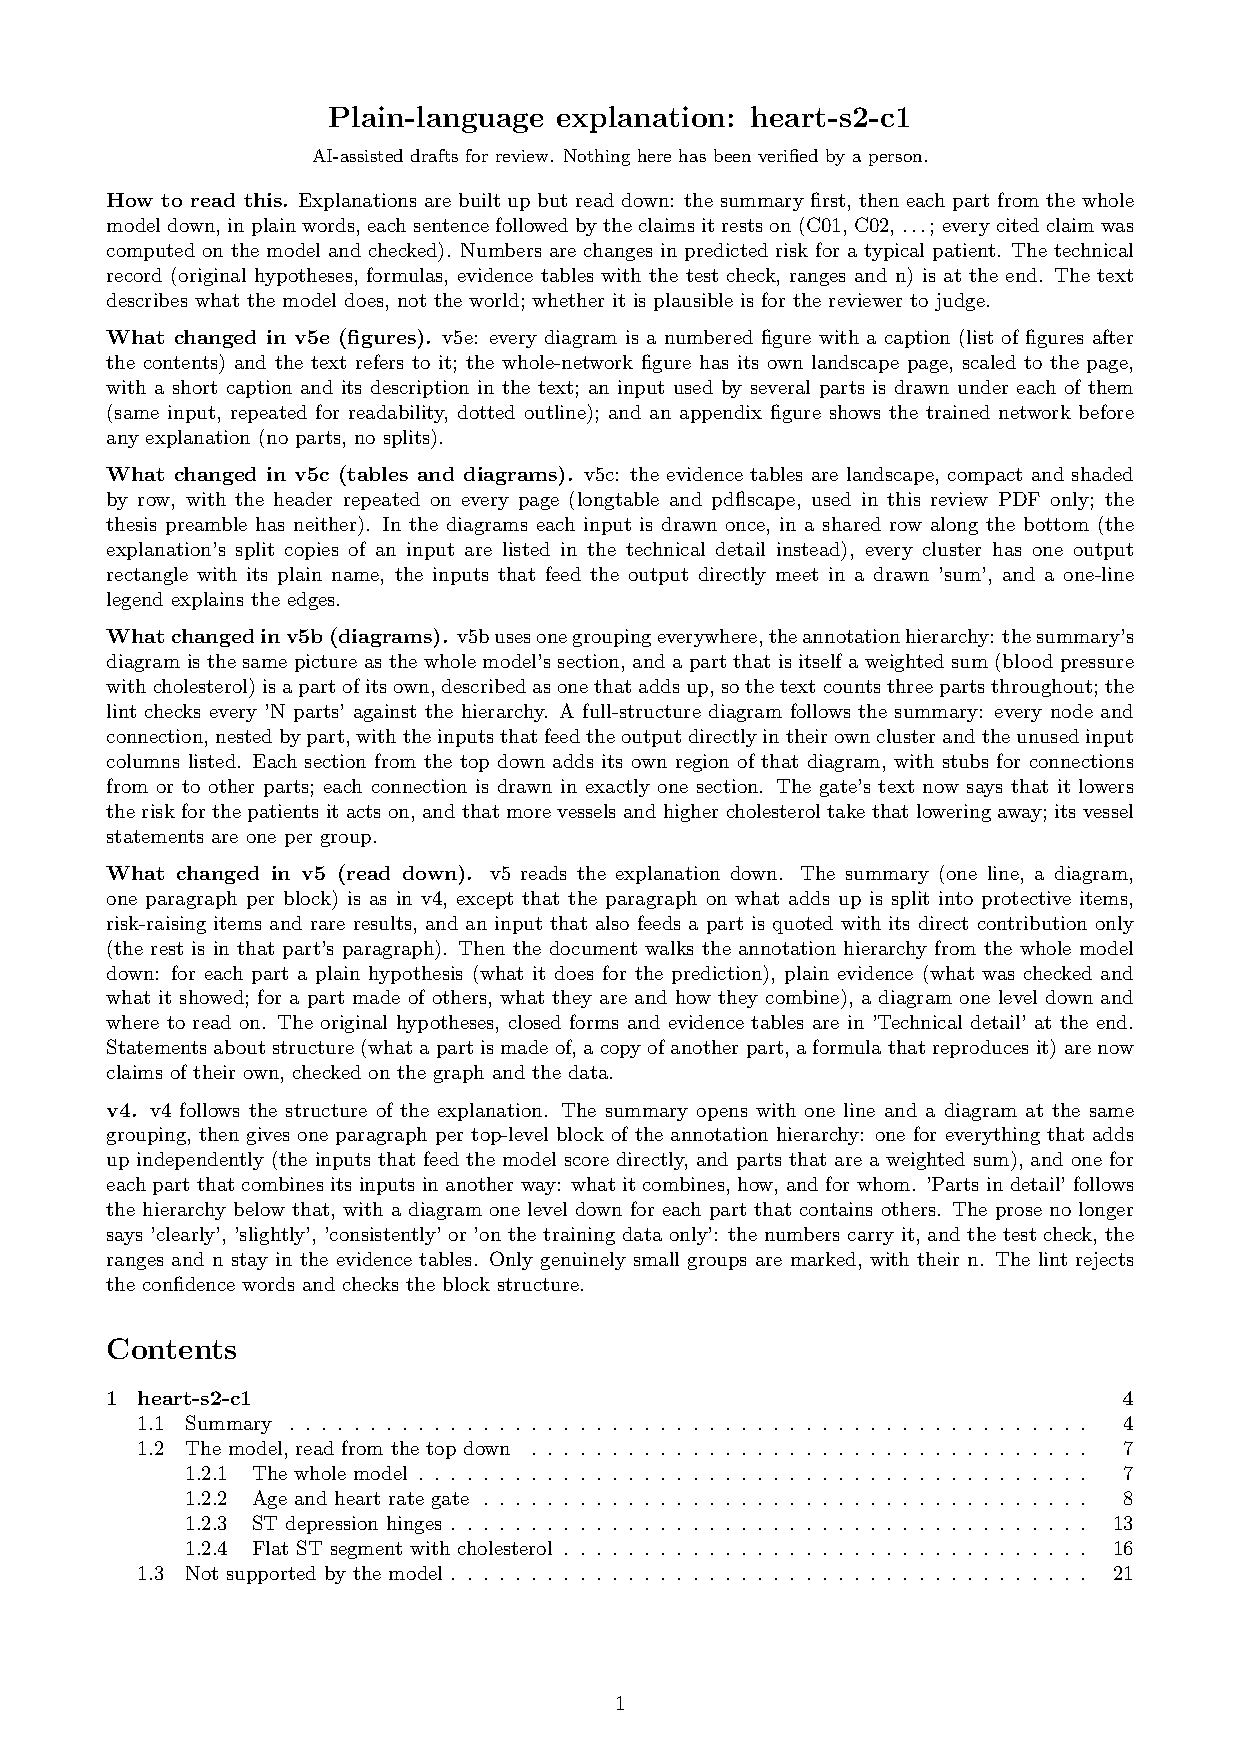
\includepdf[pages={1-5},addtotoc={1,section,1,{heart-s2-c1: plain-language explanation (read-down document)},plain:heart-s2-c1}]{heart-s2-c1/heart-s2-c1-plain-v5.pdf}
\includepdf[pages={6},landscape]{heart-s2-c1/heart-s2-c1-plain-v5.pdf}
\includepdf[pages={7-22}]{heart-s2-c1/heart-s2-c1-plain-v5.pdf}
\includepdf[pages={23-25},landscape]{heart-s2-c1/heart-s2-c1-plain-v5.pdf}
\includepdf[pages={26}]{heart-s2-c1/heart-s2-c1-plain-v5.pdf}
\includepdf[pages={27},landscape]{heart-s2-c1/heart-s2-c1-plain-v5.pdf}
\includepdf[pages={28}]{heart-s2-c1/heart-s2-c1-plain-v5.pdf}
\includepdf[pages={29},landscape]{heart-s2-c1/heart-s2-c1-plain-v5.pdf}
\includepdf[pages={30}]{heart-s2-c1/heart-s2-c1-plain-v5.pdf}
\includepdf[pages={31},landscape]{heart-s2-c1/heart-s2-c1-plain-v5.pdf}
\includepdf[pages={32}]{heart-s2-c1/heart-s2-c1-plain-v5.pdf}
\includepdf[pages={33},landscape]{heart-s2-c1/heart-s2-c1-plain-v5.pdf}
\includepdf[pages={34}]{heart-s2-c1/heart-s2-c1-plain-v5.pdf}
\addcontentsline{toc}{section}{heart-s2-c1: coverage certificate}
% Coverage certificate for heart-s2-c1 (genome 22757c22-3eac-4248-961b-ed0cd500a680); content sha256 ec79581c3744183266a79714da5938691c85a75cec2be1eb4de5c84f12391d56.
\providecommand{\explaneatcertdir}[1]{}
\begin{drafted}[heart-s2-c1 coverage certificate]
\section{Coverage certificate: heart-s2-c1}\label{app:heart-s2-c1:sec}
Provenance, coverage and checks of the explanation, rendered from the canonical JSON record \texttt{heart-s2-c1.json} (schema 1.4.0, SHA-256 \texttt{ec79581c37441832}\ldots). The explanation itself (summary, parts, evidence, figures) is the read-down document before this page.

\begin{table}[htbp]
\centering\small
\begin{tabularx}{\linewidth}{@{}lX@{}}
\toprule
Dataset & Heart Disease (binary, prepared) \\
Experiment & 10seed-heart-s2, seed 2 \\
Genome & \texttt{22757c22-3eac-4248-961b-ed0cd500a680} (NEAT key 9083, generation 39) \\
Explanation & \texttt{eac2ad3d-7d0e-4112-9d34-7f0f217a2c31} (35 operations) \\
Train AUC / accuracy & 0.9432 / 0.8802 (n = 242) \\
Test AUC / accuracy & 0.8966 / 0.8361 (n = 61) \\
Output activation & sigmoid \\
Phenotype & 33 nodes (26 inputs, 6 hidden, 1 output), 31 enabled edges \\
Explained model state & 39 nodes, 31 enabled edges \\
Refactoring operations & split\_\allowbreak{}node 5 \\
Function preservation & max $|\Delta\,\mathrm{output}|$ = $2.22\times 10^{-16}$ on the training split \\
Annotations & 4 (3 leaf, 1 composition) \\
Structural coverage & 1 (38 of 38 candidate nodes; 8 Null) \\
Compositional coverage & 1 \\
Uncovered nodes / edges & 0 / 0 \\
Missing compositions & 0 \\
Full coverage & yes \\
Drafted by & AI-assisted draft \\
Verified by & unverified \\
Record hash (SHA-256) & \texttt{ec79581c37441832}\ldots \\
\bottomrule
\end{tabularx}
\caption{Explanation certificate summary: heart-s2-c1.}
\label{app:heart-s2-c1:summary}
\end{table}
\subsection{Coverage}\label{app:heart-s2-c1:coverage}
Coverage is computed by the current code (the function behind the \texttt{get\_coverage} tool) under these conventions. \emph{Candidate nodes} are all nodes of the explained model state except the output nodes. A candidate node is \emph{covered} when some annotation of the hierarchy (a leaf, or a composition together with its descendants) contains it and all its enabled outgoing edges. \emph{Exact Null} parts, which have no effect on any output for any input, count as covered: nodes with no path to an output over enabled, non-zero-weight edges (disconnected inputs and dead ends), and edges that have zero weight or touch such a node. Compositional coverage is the fraction of required compositions present: every annotation except a single global root containing every output must have a parent; a parentless, childless annotation made only of Null nodes is exempt.

\begin{itemize}
\item \textbf{Null, disconnected input (8):} \texttt{-10} (fbs:0), \texttt{-12} (restecg:0), \texttt{-14} (restecg:2), \texttt{-16} (exang:0), \texttt{-21} (slope:3), \texttt{-23} (thal:3), \texttt{-24} (thal:4), \texttt{-6} (cp:3).
\item \textbf{Uncovered nodes:} none.
\item \textbf{Uncovered edges:} none.
\item \textbf{Missing compositions:} none.
\end{itemize}
\noindent\textbf{Agreement with the \texttt{get\_coverage} tool:} yes.

\subsection{Closed-form checks}\label{app:heart-s2-c1:closedform}
{\small\noindent\begin{tabularx}{\linewidth}{@{}lXrr@{}}
\toprule Tag & Annotation & Closed form vs forward pass & Exact function vs forward pass \\ \midrule
A1 & heart\_\allowbreak{}disease\_\allowbreak{}logit & 0.00201 & $2.22\times 10^{-16}$ \\
A2 & age\_\allowbreak{}hr\_\allowbreak{}reserve\_\allowbreak{}gate & 0.0114 & $8.88\times 10^{-16}$ \\
A3 & st\_\allowbreak{}slope\_\allowbreak{}chol\_\allowbreak{}gate & 0.00231 & $4.44\times 10^{-16}$ \\
A4 & oldpeak\_\allowbreak{}hinges & 0.0131 & 0 \\
\bottomrule
\end{tabularx}\par}
\subsection{Refactoring operations}\label{app:heart-s2-c1:operations}
The explained model state is the phenotype after these operations, replayed in order. All are function-preserving; the largest change in the model output over the 242 training rows is $2.22\times 10^{-16}$ (tolerance $1.00\times 10^{-9}$).
\begin{itemize}
\item \#26: split \texttt{-26} into \texttt{-26\_\allowbreak{}a}, \texttt{-26\_\allowbreak{}b}, \texttt{-26\_\allowbreak{}c}.
\item \#27: split \texttt{-15} into \texttt{-15\_\allowbreak{}a}, \texttt{-15\_\allowbreak{}b}.
\item \#28: split \texttt{-9} into \texttt{-9\_\allowbreak{}a}, \texttt{-9\_\allowbreak{}b}.
\item \#29: split \texttt{-20} into \texttt{-20\_\allowbreak{}a}, \texttt{-20\_\allowbreak{}b}.
\item \#30: split \texttt{-18} into \texttt{-18\_\allowbreak{}a}, \texttt{-18\_\allowbreak{}b}.
\end{itemize}
\subsection{Audit against the definitions}\label{app:heart-s2-c1:audit}
Automatic findings on the stored explanation (codes as in the JSON record's \texttt{issues}); they flag what an examiner should check, not verdicts.
\begin{itemize}
\item \textsc{warning} \texttt{unverified}: No human verification is recorded for this explanation.
\end{itemize}
\end{drafted}

\clearpage
\section*{8. heart-s2-c2: verification checklist}
\addcontentsline{toc}{section}{8. heart-s2-c2: verification checklist}
\label{rev:heart-s2-c2}
\textbf{Already recorded:} nothing (no verdict in the record).

\textbf{Recorded vs live.} Agent = the drafting agent's report; orchestrator = the record's automated re-check; live = this export (current code, training split).

{\footnotesize
\begin{tabularx}{\linewidth}{@{}>{\raggedright\arraybackslash}X>{\raggedright\arraybackslash}p{2.1cm}>{\raggedright\arraybackslash}p{3.0cm}>{\raggedright\arraybackslash}p{3.0cm}l@{}}
\toprule
Check & Agent & Orchestrator & Live & Status \\
\midrule
Function preservation, max $|$change in output$|$ & 2.22e-16 & 2.22e-16 & 2.22e-16 & agree \\
Closed-form max abs error (all leaves) & 0.005339 & 0.005339 & 0.005339 & agree \\
Numeric-function max abs error & n/a & 4.44e-16 & 4.44e-16 & agree \\
Structural coverage & 1 & 1 & 1 & agree \\
Compositional coverage & 1 & 1 & 1 & agree \\
Hierarchy complete & yes & yes & yes & agree \\
Root annotation & n/a & heart\_\allowbreak{}disease\_\allowbreak{}logit & heart\_\allowbreak{}disease\_\allowbreak{}logit & agree \\
Leaf / composition counts & 2 / 1 & n/a & 2 / 1 & agree \\
Operation counts & 2 splits, 0 identity & annotate 3, rename node 26, split node 2 & annotate 3, rename node 26, split node 2 & agree \\
Full coverage & yes & yes & yes & agree \\
\bottomrule
\end{tabularx}}

\textbf{What to look at.}
\begin{itemize}
\item Largest closed-form error: \texttt{heart\_\allowbreak{}rate\_\allowbreak{}nonanginal\_\allowbreak{}gate} (0.00534). This is the cost of the 3 s.f. display rounding, in the exit's own units; the numeric function is exact. Check that the rounded formula still supports the hypothesis as worded.
\item Strong claim in \texttt{heart\_\allowbreak{}rate\_\allowbreak{}nonanginal\_\allowbreak{}gate}: \emph{``The gate opens once max heart rate passes a threshold set by the other two inputs: about -2.3 SD with non-anginal pain (open for 66 of 68), about +0.78 SD for other pain types without a fixed defect (38 of 159), and never with a f...''} Is this (exactness, threshold, rare category) supported by the evidence, or fitted to a few rows?
\item Strong claim in \texttt{restecg2\_\allowbreak{}relay}: \emph{``exactly affine in the binary input on the data.''} Is this (exactness, threshold, rare category) supported by the evidence, or fitted to a few rows?
\item 2 split(s), all of input nodes (an input feeding two annotations). These are routine; check only that each input copy sits in the annotation whose hypothesis uses it.
\item Read the root's hypothesis against its closed form: does the stated combination of children (additive, gated, serial) match the formula?
\end{itemize}
\textbf{Tool notes (record):} No v3 tool bugs met. compute\_\allowbreak{}shap on all 242 train rows took about a minute; unconnected inputs get mean $|$SHAP$|$ about 0.0009 (KernelSHAP noise, exact effect zero). The agent sandbox refuses compound shell commands with variables, so tools were called through a small Python subprocess wrapper in scratch (same species\_\allowbreak{}leads/\allowbreak{}xn.py)\allowbreak{}.

\textbf{Plain-language layer} (AI-assisted draft for review (unverified)): the read-down document follows this page (summary, parts, evidence, worth checking; also \texttt{heart-s2-c2-plain-v5.pdf} in this genome's folder). Record a verdict on it with \texttt{uv run python -m explaneat export record-plain-verdict heart-s2-c2 --verified --minutes N --notes "..."}.

\textbf{Verdict.}

\begin{tabularx}{\linewidth}{@{}lX@{}}
Verified (correct as it stands, or after my changes): & $\square$ yes \quad $\square$ no \\[4pt]
Minutes: & \rule{3cm}{0.4pt} \\[4pt]
Changes: & \rule{\linewidth}{0.4pt} \\[10pt]
 & \rule{\linewidth}{0.4pt} \\[4pt]
Notes: & \rule{\linewidth}{0.4pt} \\[10pt]
 & \rule{\linewidth}{0.4pt} \\
\end{tabularx}

\textbf{Record it} (writes \texttt{mike\_verification} into \texttt{experiments/10seed/explanations/heart-s2-c2.json}; use \texttt{-{}-not-verified} for no; rebuild the CSVs with \texttt{uv run python experiments/10seed/build\_explanations\_csv.py}):

{\footnotesize\raggedright\texttt{uv run python -m explaneat export record-verdict heart-s2-c2 --verified --minutes N --changes "..." --notes "..."}\par}


\clearpage
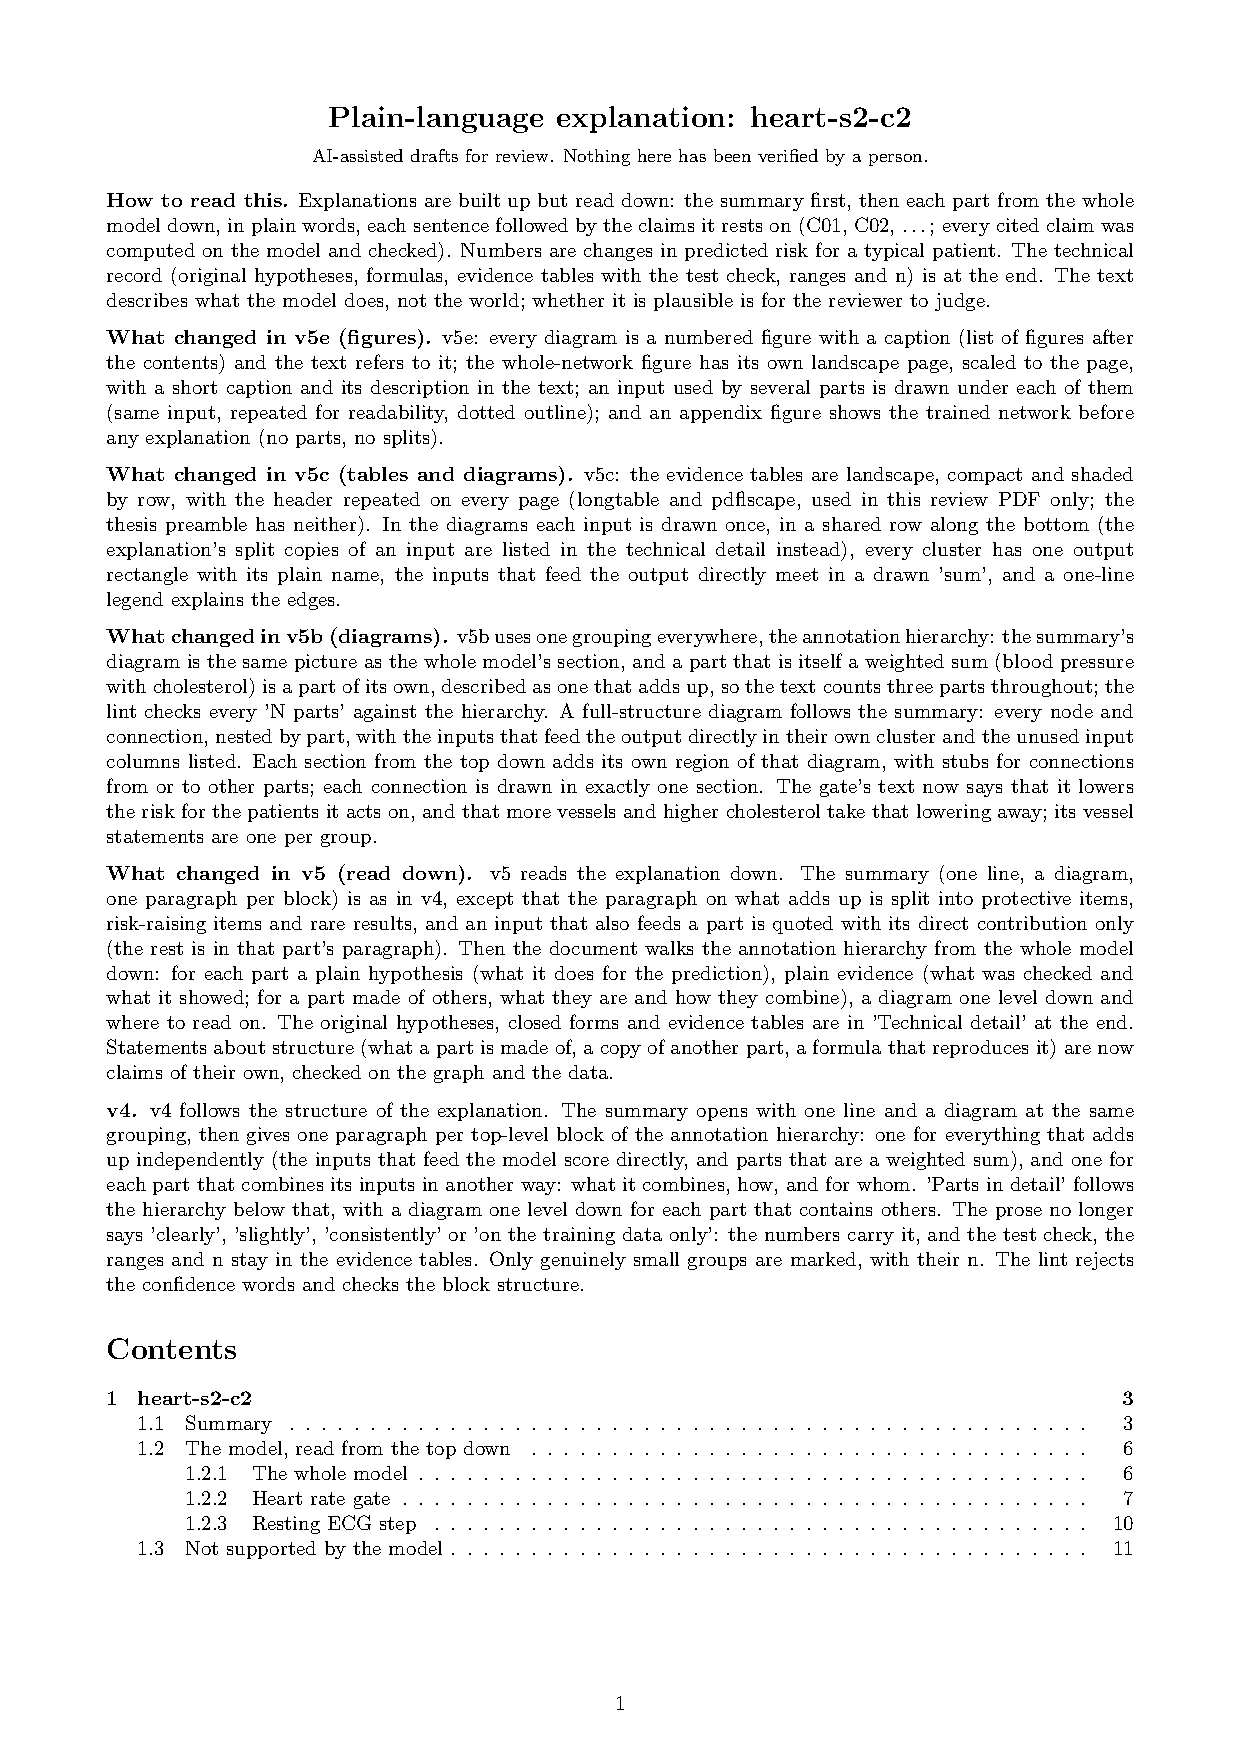
\includepdf[pages={1-4},addtotoc={1,section,1,{heart-s2-c2: plain-language explanation (read-down document)},plain:heart-s2-c2}]{heart-s2-c2/heart-s2-c2-plain-v5.pdf}
\includepdf[pages={5},landscape]{heart-s2-c2/heart-s2-c2-plain-v5.pdf}
\includepdf[pages={6-12}]{heart-s2-c2/heart-s2-c2-plain-v5.pdf}
\includepdf[pages={13-15},landscape]{heart-s2-c2/heart-s2-c2-plain-v5.pdf}
\includepdf[pages={16}]{heart-s2-c2/heart-s2-c2-plain-v5.pdf}
\includepdf[pages={17},landscape]{heart-s2-c2/heart-s2-c2-plain-v5.pdf}
\includepdf[pages={18}]{heart-s2-c2/heart-s2-c2-plain-v5.pdf}
\includepdf[pages={19},landscape]{heart-s2-c2/heart-s2-c2-plain-v5.pdf}
\includepdf[pages={20}]{heart-s2-c2/heart-s2-c2-plain-v5.pdf}
\includepdf[pages={21},landscape]{heart-s2-c2/heart-s2-c2-plain-v5.pdf}
\includepdf[pages={22}]{heart-s2-c2/heart-s2-c2-plain-v5.pdf}
\addcontentsline{toc}{section}{heart-s2-c2: coverage certificate}
% Coverage certificate for heart-s2-c2 (genome d4bbc960-816a-4781-8979-fdd4165debf2); content sha256 1276e9a13f62dbc089618dbbcbf8c7fcbf1ae0d7094c9016ac0b90a0a0c036ac.
\providecommand{\explaneatcertdir}[1]{}
\begin{drafted}[heart-s2-c2 coverage certificate]
\section{Coverage certificate: heart-s2-c2}\label{app:heart-s2-c2:sec}
Provenance, coverage and checks of the explanation, rendered from the canonical JSON record \texttt{heart-s2-c2.json} (schema 1.4.0, SHA-256 \texttt{1276e9a13f62dbc0}\ldots). The explanation itself (summary, parts, evidence, figures) is the read-down document before this page.

\begin{table}[htbp]
\centering\small
\begin{tabularx}{\linewidth}{@{}lX@{}}
\toprule
Dataset & Heart Disease (binary, prepared) \\
Experiment & 10seed-heart-s2, seed 2 \\
Genome & \texttt{d4bbc960-816a-4781-8979-fdd4165debf2} (NEAT key 9685, generation 39) \\
Explanation & \texttt{3531d96c-aa00-4141-863a-2c85155afe8f} (31 operations) \\
Train AUC / accuracy & 0.9403 / 0.8967 (n = 242) \\
Test AUC / accuracy & 0.9009 / 0.8197 (n = 61) \\
Output activation & sigmoid \\
Phenotype & 31 nodes (26 inputs, 4 hidden, 1 output), 24 enabled edges \\
Explained model state & 33 nodes, 24 enabled edges \\
Refactoring operations & split\_\allowbreak{}node 2 \\
Function preservation & max $|\Delta\,\mathrm{output}|$ = $2.22\times 10^{-16}$ on the training split \\
Annotations & 3 (2 leaf, 1 composition) \\
Structural coverage & 1 (32 of 32 candidate nodes; 8 Null) \\
Compositional coverage & 1 \\
Uncovered nodes / edges & 0 / 0 \\
Missing compositions & 0 \\
Full coverage & yes \\
Drafted by & AI-assisted draft \\
Verified by & unverified \\
Record hash (SHA-256) & \texttt{1276e9a13f62dbc0}\ldots \\
\bottomrule
\end{tabularx}
\caption{Explanation certificate summary: heart-s2-c2.}
\label{app:heart-s2-c2:summary}
\end{table}
\subsection{Coverage}\label{app:heart-s2-c2:coverage}
Coverage is computed by the current code (the function behind the \texttt{get\_coverage} tool) under these conventions. \emph{Candidate nodes} are all nodes of the explained model state except the output nodes. A candidate node is \emph{covered} when some annotation of the hierarchy (a leaf, or a composition together with its descendants) contains it and all its enabled outgoing edges. \emph{Exact Null} parts, which have no effect on any output for any input, count as covered: nodes with no path to an output over enabled, non-zero-weight edges (disconnected inputs and dead ends), and edges that have zero weight or touch such a node. Compositional coverage is the fraction of required compositions present: every annotation except a single global root containing every output must have a parent; a parentless, childless annotation made only of Null nodes is exempt.

\begin{itemize}
\item \textbf{Null, disconnected input (8):} \texttt{-10} (fbs:0), \texttt{-12} (restecg:0), \texttt{-13} (restecg:1), \texttt{-16} (exang:0), \texttt{-17} (exang:1), \texttt{-21} (slope:3), \texttt{-23} (thal:3), \texttt{-24} (thal:4).
\item \textbf{Uncovered nodes:} none.
\item \textbf{Uncovered edges:} none.
\item \textbf{Missing compositions:} none.
\end{itemize}
\noindent\textbf{Agreement with the \texttt{get\_coverage} tool:} yes.

\subsection{Closed-form checks}\label{app:heart-s2-c2:closedform}
{\small\noindent\begin{tabularx}{\linewidth}{@{}lXrr@{}}
\toprule Tag & Annotation & Closed form vs forward pass & Exact function vs forward pass \\ \midrule
A1 & heart\_\allowbreak{}disease\_\allowbreak{}logit & $8.94\times 10^{-4}$ & $2.22\times 10^{-16}$ \\
A2 & heart\_\allowbreak{}rate\_\allowbreak{}nonanginal\_\allowbreak{}gate & 0.00534 & $4.44\times 10^{-16}$ \\
A3 & restecg2\_\allowbreak{}relay & $1.39\times 10^{-4}$ & 0 \\
\bottomrule
\end{tabularx}\par}
\subsection{Refactoring operations}\label{app:heart-s2-c2:operations}
The explained model state is the phenotype after these operations, replayed in order. All are function-preserving; the largest change in the model output over the 242 training rows is $2.22\times 10^{-16}$ (tolerance $1.00\times 10^{-9}$).
\begin{itemize}
\item \#26: split \texttt{-15} into \texttt{-15\_\allowbreak{}a}, \texttt{-15\_\allowbreak{}b}.
\item \#27: split \texttt{-25} into \texttt{-25\_\allowbreak{}a}, \texttt{-25\_\allowbreak{}b}.
\end{itemize}
\subsection{Audit against the definitions}\label{app:heart-s2-c2:audit}
Automatic findings on the stored explanation (codes as in the JSON record's \texttt{issues}); they flag what an examiner should check, not verdicts.
\begin{itemize}
\item \textsc{warning} \texttt{unverified}: No human verification is recorded for this explanation.
\end{itemize}
\end{drafted}

\clearpage
\section*{9. heart-s2-c3: verification checklist}
\addcontentsline{toc}{section}{9. heart-s2-c3: verification checklist}
\label{rev:heart-s2-c3}
\textbf{Already recorded:} nothing (no verdict in the record).

\textbf{Recorded vs live.} Agent = the drafting agent's report; orchestrator = the record's automated re-check; live = this export (current code, training split).

{\footnotesize
\begin{tabularx}{\linewidth}{@{}>{\raggedright\arraybackslash}X>{\raggedright\arraybackslash}p{2.1cm}>{\raggedright\arraybackslash}p{3.0cm}>{\raggedright\arraybackslash}p{3.0cm}l@{}}
\toprule
Check & Agent & Orchestrator & Live & Status \\
\midrule
Function preservation, max $|$change in output$|$ & 2.22e-16 & 2.22e-16 & 2.22e-16 & agree \\
Closed-form max abs error (all leaves) & 0.006749 & 0.006749 & 0.006749 & agree \\
Numeric-function max abs error & n/a & 0 & 0 & agree \\
Structural coverage & 1 & 1 & 1 & agree \\
Compositional coverage & 1 & 1 & 1 & agree \\
Hierarchy complete & yes & yes & yes & agree \\
Root annotation & n/a & heart\_\allowbreak{}disease\_\allowbreak{}logit & heart\_\allowbreak{}disease\_\allowbreak{}logit & agree \\
Leaf / composition counts & 3 / 1 & n/a & 3 / 1 & agree \\
Operation counts & 4 splits, 0 identity & annotate 4, rename node 26, split node 4 & annotate 4, rename node 26, split node 4 & agree \\
Full coverage & yes & yes & yes & agree \\
\bottomrule
\end{tabularx}}

\textbf{What to look at.}
\begin{itemize}
\item Largest closed-form error: \texttt{nonanginal\_\allowbreak{}thalach\_\allowbreak{}gate} (0.00675). This is the cost of the 3 s.f. display rounding, in the exit's own units; the numeric function is exact. Check that the rounded formula still supports the hypothesis as worded.
\item Strong claim in \texttt{nonanginal\_\allowbreak{}thalach\_\allowbreak{}gate}: \emph{``...(train, n=242): active for 97\% of the 70 non-anginal-pain patients (closed only for z-thalach $<$ -1.97) and 5\% of the 172 others (only z-thalach $>$ 1.53).''} Is this (exactness, threshold, rare category) supported by the evidence, or fitted to a few rows?
\item 4 split(s), all of input nodes (an input feeding two annotations). These are routine; check only that each input copy sits in the annotation whose hypothesis uses it.
\item Read the root's hypothesis against its closed form: does the stated combination of children (additive, gated, serial) match the formula?
\end{itemize}
\textbf{Tool notes (record):} No v3 tool bugs met. compute\_\allowbreak{}shap on all 242 train rows took about a minute; it gives the nine unconnected inputs mean $|$SHAP$|$ about 0.001 (estimator noise, not an effect). The agent sandbox refused shell loops calling uv with variables, so tools were called through a small Python subprocess wrapper in scratch (same xn.py). Input fan-out splits (-6, -15, -18, -9) taken from the topology and detect\_\allowbreak{}splits.

\textbf{Plain-language layer} (AI-assisted draft for review (unverified)): the read-down document follows this page (summary, parts, evidence, worth checking; also \texttt{heart-s2-c3-plain-v5.pdf} in this genome's folder). Record a verdict on it with \texttt{uv run python -m explaneat export record-plain-verdict heart-s2-c3 --verified --minutes N --notes "..."}.

\textbf{Verdict.}

\begin{tabularx}{\linewidth}{@{}lX@{}}
Verified (correct as it stands, or after my changes): & $\square$ yes \quad $\square$ no \\[4pt]
Minutes: & \rule{3cm}{0.4pt} \\[4pt]
Changes: & \rule{\linewidth}{0.4pt} \\[10pt]
 & \rule{\linewidth}{0.4pt} \\[4pt]
Notes: & \rule{\linewidth}{0.4pt} \\[10pt]
 & \rule{\linewidth}{0.4pt} \\
\end{tabularx}

\textbf{Record it} (writes \texttt{mike\_verification} into \texttt{experiments/10seed/explanations/heart-s2-c3.json}; use \texttt{-{}-not-verified} for no; rebuild the CSVs with \texttt{uv run python experiments/10seed/build\_explanations\_csv.py}):

{\footnotesize\raggedright\texttt{uv run python -m explaneat export record-verdict heart-s2-c3 --verified --minutes N --changes "..." --notes "..."}\par}


\clearpage
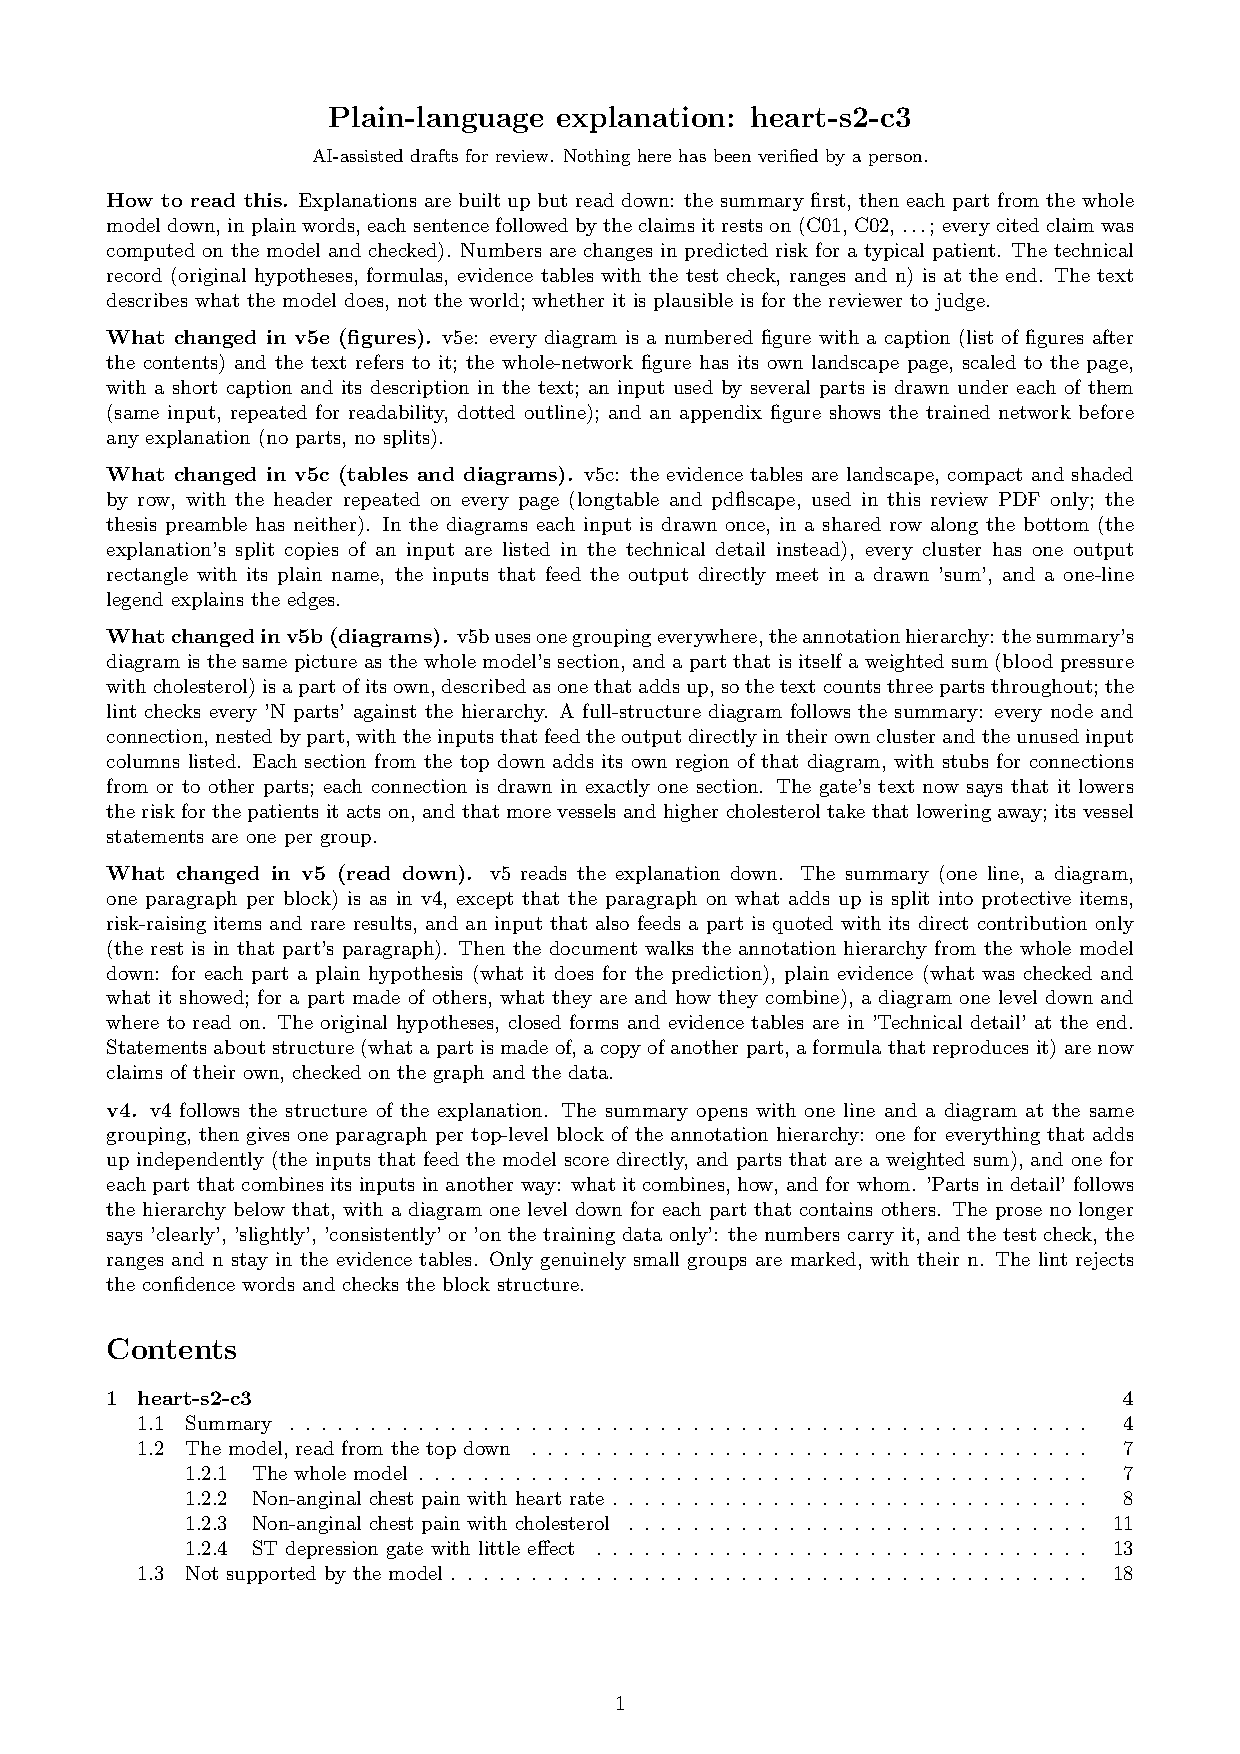
\includepdf[pages={1-5},addtotoc={1,section,1,{heart-s2-c3: plain-language explanation (read-down document)},plain:heart-s2-c3}]{heart-s2-c3/heart-s2-c3-plain-v5.pdf}
\includepdf[pages={6},landscape]{heart-s2-c3/heart-s2-c3-plain-v5.pdf}
\includepdf[pages={7-19}]{heart-s2-c3/heart-s2-c3-plain-v5.pdf}
\includepdf[pages={20-21},landscape]{heart-s2-c3/heart-s2-c3-plain-v5.pdf}
\includepdf[pages={22}]{heart-s2-c3/heart-s2-c3-plain-v5.pdf}
\includepdf[pages={23},landscape]{heart-s2-c3/heart-s2-c3-plain-v5.pdf}
\includepdf[pages={24}]{heart-s2-c3/heart-s2-c3-plain-v5.pdf}
\includepdf[pages={25},landscape]{heart-s2-c3/heart-s2-c3-plain-v5.pdf}
\includepdf[pages={26}]{heart-s2-c3/heart-s2-c3-plain-v5.pdf}
\includepdf[pages={27},landscape]{heart-s2-c3/heart-s2-c3-plain-v5.pdf}
\includepdf[pages={28}]{heart-s2-c3/heart-s2-c3-plain-v5.pdf}
\includepdf[pages={29},landscape]{heart-s2-c3/heart-s2-c3-plain-v5.pdf}
\includepdf[pages={30}]{heart-s2-c3/heart-s2-c3-plain-v5.pdf}
\addcontentsline{toc}{section}{heart-s2-c3: coverage certificate}
% Coverage certificate for heart-s2-c3 (genome 1a5255ec-4f4d-4ff4-916a-1b5c4622ccc9); content sha256 6b36c4ae4f91161350a650f7da79e66ec93b2fa97254ec7aeab35bbb6828150b.
\providecommand{\explaneatcertdir}[1]{}
\begin{drafted}[heart-s2-c3 coverage certificate]
\section{Coverage certificate: heart-s2-c3}\label{app:heart-s2-c3:sec}
Provenance, coverage and checks of the explanation, rendered from the canonical JSON record \texttt{heart-s2-c3.json} (schema 1.4.0, SHA-256 \texttt{6b36c4ae4f911613}\ldots). The explanation itself (summary, parts, evidence, figures) is the read-down document before this page.

\begin{table}[htbp]
\centering\small
\begin{tabularx}{\linewidth}{@{}lX@{}}
\toprule
Dataset & Heart Disease (binary, prepared) \\
Experiment & 10seed-heart-s2, seed 2 \\
Genome & \texttt{1a5255ec-4f4d-4ff4-916a-1b5c4622ccc9} (NEAT key 9600, generation 39) \\
Explanation & \texttt{6565cffd-9c19-4ae2-b635-a2e35f3d485a} (34 operations) \\
Train AUC / accuracy & 0.9381 / 0.8884 (n = 242) \\
Test AUC / accuracy & 0.8987 / 0.8197 (n = 61) \\
Output activation & sigmoid \\
Phenotype & 30 nodes (26 inputs, 3 hidden, 1 output), 26 enabled edges \\
Explained model state & 36 nodes, 26 enabled edges \\
Refactoring operations & split\_\allowbreak{}node 4 \\
Function preservation & max $|\Delta\,\mathrm{output}|$ = $2.22\times 10^{-16}$ on the training split \\
Annotations & 4 (3 leaf, 1 composition) \\
Structural coverage & 1 (35 of 35 candidate nodes; 9 Null) \\
Compositional coverage & 1 \\
Uncovered nodes / edges & 0 / 0 \\
Missing compositions & 0 \\
Full coverage & yes \\
Drafted by & AI-assisted draft \\
Verified by & unverified \\
Record hash (SHA-256) & \texttt{6b36c4ae4f911613}\ldots \\
\bottomrule
\end{tabularx}
\caption{Explanation certificate summary: heart-s2-c3.}
\label{app:heart-s2-c3:summary}
\end{table}
\subsection{Coverage}\label{app:heart-s2-c3:coverage}
Coverage is computed by the current code (the function behind the \texttt{get\_coverage} tool) under these conventions. \emph{Candidate nodes} are all nodes of the explained model state except the output nodes. A candidate node is \emph{covered} when some annotation of the hierarchy (a leaf, or a composition together with its descendants) contains it and all its enabled outgoing edges. \emph{Exact Null} parts, which have no effect on any output for any input, count as covered: nodes with no path to an output over enabled, non-zero-weight edges (disconnected inputs and dead ends), and edges that have zero weight or touch such a node. Compositional coverage is the fraction of required compositions present: every annotation except a single global root containing every output must have a parent; a parentless, childless annotation made only of Null nodes is exempt.

\begin{itemize}
\item \textbf{Null, disconnected input (9):} \texttt{-1} (age), \texttt{-10} (fbs:0), \texttt{-12} (restecg:0), \texttt{-13} (restecg:1), \texttt{-16} (exang:0), \texttt{-17} (exang:1), \texttt{-21} (slope:3), \texttt{-23} (thal:3), \texttt{-24} (thal:4).
\item \textbf{Uncovered nodes:} none.
\item \textbf{Uncovered edges:} none.
\item \textbf{Missing compositions:} none.
\end{itemize}
\noindent\textbf{Agreement with the \texttt{get\_coverage} tool:} yes.

\subsection{Closed-form checks}\label{app:heart-s2-c3:closedform}
{\small\noindent\begin{tabularx}{\linewidth}{@{}lXrr@{}}
\toprule Tag & Annotation & Closed form vs forward pass & Exact function vs forward pass \\ \midrule
A1 & heart\_\allowbreak{}disease\_\allowbreak{}logit & 0.00141 & $2.22\times 10^{-16}$ \\
A2 & nonanginal\_\allowbreak{}thalach\_\allowbreak{}gate & 0.00675 & 0 \\
A3 & oldpeak\_\allowbreak{}gate\_\allowbreak{}without\_\allowbreak{}nonanginal & 0.00186 & 0 \\
A4 & nonanginal\_\allowbreak{}low\_\allowbreak{}chol\_\allowbreak{}gate & 0.00471 & 0 \\
\bottomrule
\end{tabularx}\par}
\subsection{Refactoring operations}\label{app:heart-s2-c3:operations}
The explained model state is the phenotype after these operations, replayed in order. All are function-preserving; the largest change in the model output over the 242 training rows is $2.22\times 10^{-16}$ (tolerance $1.00\times 10^{-9}$).
\begin{itemize}
\item \#26: split \texttt{-6} into \texttt{-6\_\allowbreak{}a}, \texttt{-6\_\allowbreak{}b}, \texttt{-6\_\allowbreak{}c}.
\item \#27: split \texttt{-15} into \texttt{-15\_\allowbreak{}a}, \texttt{-15\_\allowbreak{}b}, \texttt{-15\_\allowbreak{}c}.
\item \#28: split \texttt{-18} into \texttt{-18\_\allowbreak{}a}, \texttt{-18\_\allowbreak{}b}.
\item \#29: split \texttt{-9} into \texttt{-9\_\allowbreak{}a}, \texttt{-9\_\allowbreak{}b}.
\end{itemize}
\subsection{Audit against the definitions}\label{app:heart-s2-c3:audit}
Automatic findings on the stored explanation (codes as in the JSON record's \texttt{issues}); they flag what an examiner should check, not verdicts.
\begin{itemize}
\item \textsc{warning} \texttt{unverified}: No human verification is recorded for this explanation.
\end{itemize}
\end{drafted}

\clearpage
\section*{10. heart-s4-c1: verification checklist}
\addcontentsline{toc}{section}{10. heart-s4-c1: verification checklist}
\label{rev:heart-s4-c1}
\textbf{Already recorded:} nothing (no verdict in the record).

\textbf{Recorded vs live.} Agent = the drafting agent's report; orchestrator = the record's automated re-check; live = this export (current code, training split).

{\footnotesize
\begin{tabularx}{\linewidth}{@{}>{\raggedright\arraybackslash}X>{\raggedright\arraybackslash}p{2.1cm}>{\raggedright\arraybackslash}p{3.0cm}>{\raggedright\arraybackslash}p{3.0cm}l@{}}
\toprule
Check & Agent & Orchestrator & Live & Status \\
\midrule
Function preservation, max $|$change in output$|$ & 3.33e-16 & 3.33e-16 & 3.33e-16 & agree \\
Closed-form max abs error (all leaves) & 0.001728 & 0.001728 & 0.001728 & agree \\
Numeric-function max abs error & n/a & 0 & 0 & agree \\
Structural coverage & 1 & 1 & 1 & agree \\
Compositional coverage & 1 & 1 & 1 & agree \\
Hierarchy complete & yes & yes & yes & agree \\
Root annotation & n/a & heart\_\allowbreak{}disease\_\allowbreak{}logit & heart\_\allowbreak{}disease\_\allowbreak{}logit & agree \\
Leaf / composition counts & 4 / 1 & n/a & 4 / 1 & agree \\
Operation counts & 5 splits, 0 identity & annotate 5, rename node 26, split node 5 & annotate 5, rename node 26, split node 5 & agree \\
Full coverage & yes & yes & yes & agree \\
\bottomrule
\end{tabularx}}

\textbf{What to look at.}
\begin{itemize}
\item Largest closed-form error: \texttt{no\_\allowbreak{}asymptomatic\_\allowbreak{}pain\_\allowbreak{}indicator} (0.00173). This is the cost of the 3 s.f. display rounding, in the exit's own units; the numeric function is exact. Check that the rounded formula still supports the hypothesis as worded.
\item Strong claim in \texttt{fixed\_\allowbreak{}defect\_\allowbreak{}normal\_\allowbreak{}sugar\_\allowbreak{}gate}: \emph{``EVIDENCE (train, n=242): exact on-data reduction 2065 = 3.639*[thal:6=1 AND fbs=0] (fbs=1 drives the pre-activation to $<$= -6.39).''} Is this (exactness, threshold, rare category) supported by the evidence, or fitted to a few rows?
\item Strong claim in \texttt{no\_\allowbreak{}asymptomatic\_\allowbreak{}pain\_\allowbreak{}indicator}: \emph{``because cp:4 is binary it is exactly affine on the data, so it only adds to the cp:4 direct edge (+0.308 per z-unit): together, asymptomatic chest pain raises the logit by 1.47 relative to the other pain types.''} Is this (exactness, threshold, rare category) supported by the evidence, or fitted to a few rows?
\item 5 split(s), all of input nodes (an input feeding two annotations). These are routine; check only that each input copy sits in the annotation whose hypothesis uses it.
\item Read the root's hypothesis against its closed form: does the stated combination of children (additive, gated, serial) match the formula?
\end{itemize}
\textbf{Tool notes (record):} No v3 tool bugs met. compute\_\allowbreak{}shap on all 242 train rows (about a minute) gives mean $|$SHAP$|$ about 0.001 to the six unconnected inputs, which have exactly zero effect (KernelSHAP sampling noise). Input fan-out splits (-10, -11, -15, -21, -7) taken from the topology. The agent sandbox refused shell loops calling uv with variables, so tools were called through a small Python subprocess wrapper in scratch (same species\_\allowbreak{}leads/\allowbreak{}xn.py)\allowbreak{}.

\textbf{Plain-language layer} (AI-assisted draft for review (unverified)): the read-down document follows this page (summary, parts, evidence, worth checking; also \texttt{heart-s4-c1-plain-v5.pdf} in this genome's folder). Record a verdict on it with \texttt{uv run python -m explaneat export record-plain-verdict heart-s4-c1 --verified --minutes N --notes "..."}.

\textbf{Verdict.}

\begin{tabularx}{\linewidth}{@{}lX@{}}
Verified (correct as it stands, or after my changes): & $\square$ yes \quad $\square$ no \\[4pt]
Minutes: & \rule{3cm}{0.4pt} \\[4pt]
Changes: & \rule{\linewidth}{0.4pt} \\[10pt]
 & \rule{\linewidth}{0.4pt} \\[4pt]
Notes: & \rule{\linewidth}{0.4pt} \\[10pt]
 & \rule{\linewidth}{0.4pt} \\
\end{tabularx}

\textbf{Record it} (writes \texttt{mike\_verification} into \texttt{experiments/10seed/explanations/heart-s4-c1.json}; use \texttt{-{}-not-verified} for no; rebuild the CSVs with \texttt{uv run python experiments/10seed/build\_explanations\_csv.py}):

{\footnotesize\raggedright\texttt{uv run python -m explaneat export record-verdict heart-s4-c1 --verified --minutes N --changes "..." --notes "..."}\par}


\clearpage
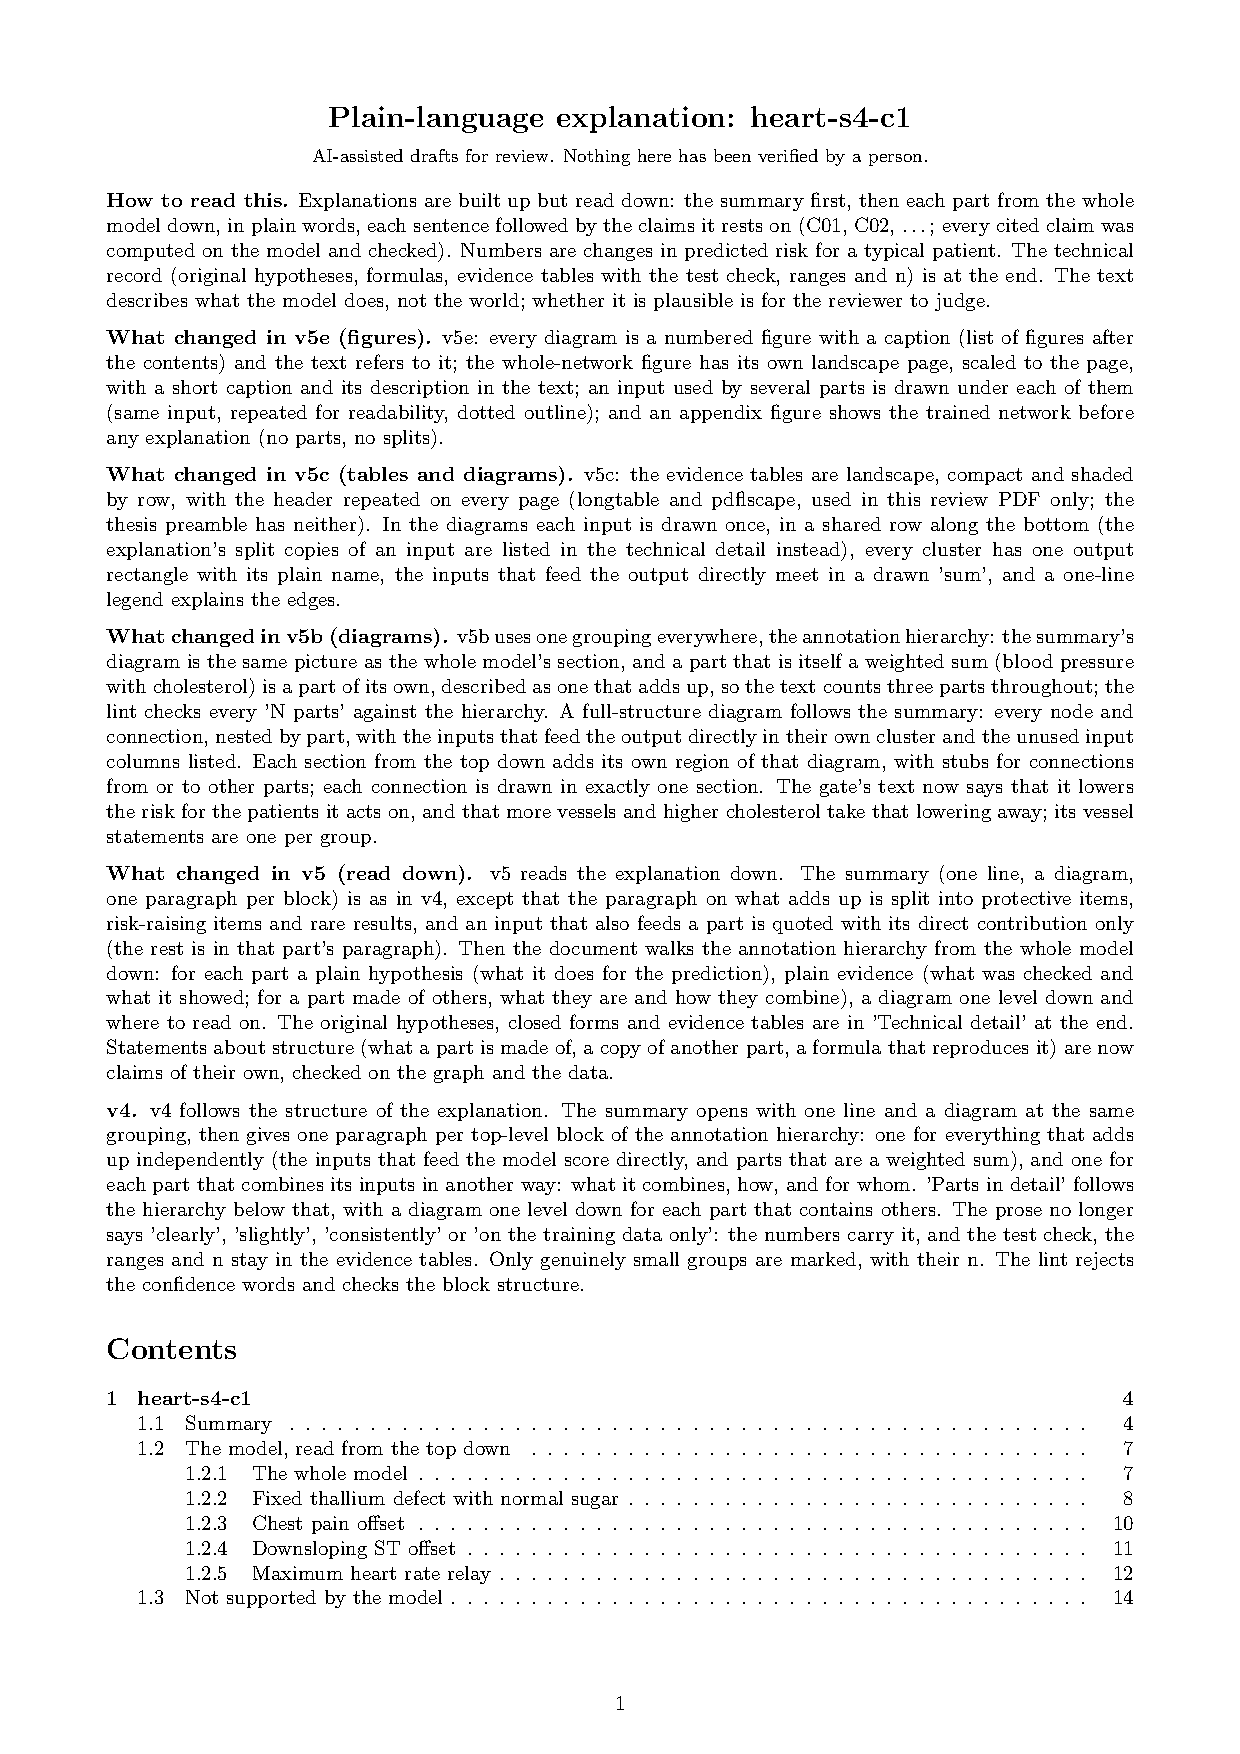
\includepdf[pages={1-5},addtotoc={1,section,1,{heart-s4-c1: plain-language explanation (read-down document)},plain:heart-s4-c1}]{heart-s4-c1/heart-s4-c1-plain-v5.pdf}
\includepdf[pages={6},landscape]{heart-s4-c1/heart-s4-c1-plain-v5.pdf}
\includepdf[pages={7-15}]{heart-s4-c1/heart-s4-c1-plain-v5.pdf}
\includepdf[pages={16-18},landscape]{heart-s4-c1/heart-s4-c1-plain-v5.pdf}
\includepdf[pages={19}]{heart-s4-c1/heart-s4-c1-plain-v5.pdf}
\includepdf[pages={20},landscape]{heart-s4-c1/heart-s4-c1-plain-v5.pdf}
\includepdf[pages={21}]{heart-s4-c1/heart-s4-c1-plain-v5.pdf}
\includepdf[pages={22},landscape]{heart-s4-c1/heart-s4-c1-plain-v5.pdf}
\includepdf[pages={23}]{heart-s4-c1/heart-s4-c1-plain-v5.pdf}
\includepdf[pages={24},landscape]{heart-s4-c1/heart-s4-c1-plain-v5.pdf}
\includepdf[pages={25}]{heart-s4-c1/heart-s4-c1-plain-v5.pdf}
\includepdf[pages={26},landscape]{heart-s4-c1/heart-s4-c1-plain-v5.pdf}
\includepdf[pages={27}]{heart-s4-c1/heart-s4-c1-plain-v5.pdf}
\includepdf[pages={28},landscape]{heart-s4-c1/heart-s4-c1-plain-v5.pdf}
\includepdf[pages={29}]{heart-s4-c1/heart-s4-c1-plain-v5.pdf}
\addcontentsline{toc}{section}{heart-s4-c1: coverage certificate}
% Coverage certificate for heart-s4-c1 (genome c85804fa-08bd-4207-ac69-a31a8567473c); content sha256 5bb264e6720c1a25b94714c430f44b3b1f28f41592eef373c0a2d422a381b5a0.
\providecommand{\explaneatcertdir}[1]{}
\begin{drafted}[heart-s4-c1 coverage certificate]
\section{Coverage certificate: heart-s4-c1}\label{app:heart-s4-c1:sec}
Provenance, coverage and checks of the explanation, rendered from the canonical JSON record \texttt{heart-s4-c1.json} (schema 1.4.0, SHA-256 \texttt{5bb264e6720c1a25}\ldots). The explanation itself (summary, parts, evidence, figures) is the read-down document before this page.

\begin{table}[htbp]
\centering\small
\begin{tabularx}{\linewidth}{@{}lX@{}}
\toprule
Dataset & Heart Disease (binary, prepared) \\
Experiment & 10seed-heart-s4, seed 4 \\
Genome & \texttt{c85804fa-08bd-4207-ac69-a31a8567473c} (NEAT key 9679, generation 39) \\
Explanation & \texttt{10565a81-f55b-47f4-b51e-21641ec08556} (36 operations) \\
Train AUC / accuracy & 0.9423 / 0.8884 (n = 242) \\
Test AUC / accuracy & 0.8858 / 0.8197 (n = 61) \\
Output activation & sigmoid \\
Phenotype & 31 nodes (26 inputs, 4 hidden, 1 output), 29 enabled edges \\
Explained model state & 36 nodes, 29 enabled edges \\
Refactoring operations & split\_\allowbreak{}node 5 \\
Function preservation & max $|\Delta\,\mathrm{output}|$ = $3.33\times 10^{-16}$ on the training split \\
Annotations & 5 (4 leaf, 1 composition) \\
Structural coverage & 1 (35 of 35 candidate nodes; 6 Null) \\
Compositional coverage & 1 \\
Uncovered nodes / edges & 0 / 0 \\
Missing compositions & 0 \\
Full coverage & yes \\
Drafted by & AI-assisted draft \\
Verified by & unverified \\
Record hash (SHA-256) & \texttt{5bb264e6720c1a25}\ldots \\
\bottomrule
\end{tabularx}
\caption{Explanation certificate summary: heart-s4-c1.}
\label{app:heart-s4-c1:summary}
\end{table}
\subsection{Coverage}\label{app:heart-s4-c1:coverage}
Coverage is computed by the current code (the function behind the \texttt{get\_coverage} tool) under these conventions. \emph{Candidate nodes} are all nodes of the explained model state except the output nodes. A candidate node is \emph{covered} when some annotation of the hierarchy (a leaf, or a composition together with its descendants) contains it and all its enabled outgoing edges. \emph{Exact Null} parts, which have no effect on any output for any input, count as covered: nodes with no path to an output over enabled, non-zero-weight edges (disconnected inputs and dead ends), and edges that have zero weight or touch such a node. Compositional coverage is the fraction of required compositions present: every annotation except a single global root containing every output must have a parent; a parentless, childless annotation made only of Null nodes is exempt.

\begin{itemize}
\item \textbf{Null, disconnected input (6):} \texttt{-12} (restecg:0), \texttt{-14} (restecg:2), \texttt{-16} (exang:0), \texttt{-24} (thal:4), \texttt{-26} (thal:7), \texttt{-5} (cp:2).
\item \textbf{Uncovered nodes:} none.
\item \textbf{Uncovered edges:} none.
\item \textbf{Missing compositions:} none.
\end{itemize}
\noindent\textbf{Agreement with the \texttt{get\_coverage} tool:} yes.

\subsection{Closed-form checks}\label{app:heart-s4-c1:closedform}
{\small\noindent\begin{tabularx}{\linewidth}{@{}lXrr@{}}
\toprule Tag & Annotation & Closed form vs forward pass & Exact function vs forward pass \\ \midrule
A1 & heart\_\allowbreak{}disease\_\allowbreak{}logit & 0.00419 & $2.78\times 10^{-16}$ \\
A2 & fixed\_\allowbreak{}defect\_\allowbreak{}normal\_\allowbreak{}sugar\_\allowbreak{}gate & $4.34\times 10^{-4}$ & 0 \\
A3 & no\_\allowbreak{}asymptomatic\_\allowbreak{}pain\_\allowbreak{}indicator & 0.00173 & 0 \\
A4 & downsloping\_\allowbreak{}st\_\allowbreak{}indicator & $1.95\times 10^{-4}$ & 0 \\
A5 & thalach\_\allowbreak{}floor\_\allowbreak{}relay & $8.60\times 10^{-4}$ & 0 \\
\bottomrule
\end{tabularx}\par}
\subsection{Refactoring operations}\label{app:heart-s4-c1:operations}
The explained model state is the phenotype after these operations, replayed in order. All are function-preserving; the largest change in the model output over the 242 training rows is $3.33\times 10^{-16}$ (tolerance $1.00\times 10^{-9}$).
\begin{itemize}
\item \#26: split \texttt{-10} into \texttt{-10\_\allowbreak{}a}, \texttt{-10\_\allowbreak{}b}.
\item \#27: split \texttt{-11} into \texttt{-11\_\allowbreak{}a}, \texttt{-11\_\allowbreak{}b}.
\item \#28: split \texttt{-15} into \texttt{-15\_\allowbreak{}a}, \texttt{-15\_\allowbreak{}b}.
\item \#29: split \texttt{-21} into \texttt{-21\_\allowbreak{}a}, \texttt{-21\_\allowbreak{}b}.
\item \#30: split \texttt{-7} into \texttt{-7\_\allowbreak{}a}, \texttt{-7\_\allowbreak{}b}.
\end{itemize}
\subsection{Audit against the definitions}\label{app:heart-s4-c1:audit}
Automatic findings on the stored explanation (codes as in the JSON record's \texttt{issues}); they flag what an examiner should check, not verdicts.
\begin{itemize}
\item \textsc{warning} \texttt{unverified}: No human verification is recorded for this explanation.
\end{itemize}
\end{drafted}

\clearpage
\section*{11. heart-s5-c1: verification checklist}
\addcontentsline{toc}{section}{11. heart-s5-c1: verification checklist}
\label{rev:heart-s5-c1}
\textbf{Already recorded:} nothing (no verdict in the record).

\textbf{Errata applied 2026-11-11}: 2 correction(s), see \texttt{experiments/\allowbreak{}errata/\allowbreak{}2026-11-11/\allowbreak{}ERRATA.md}.

\textbf{Recorded vs live.} Agent = the drafting agent's report; orchestrator = the record's automated re-check; live = this export (current code, training split).

{\footnotesize
\begin{tabularx}{\linewidth}{@{}>{\raggedright\arraybackslash}X>{\raggedright\arraybackslash}p{2.1cm}>{\raggedright\arraybackslash}p{3.0cm}>{\raggedright\arraybackslash}p{3.0cm}l@{}}
\toprule
Check & Agent & Orchestrator & Live & Status \\
\midrule
Function preservation, max $|$change in output$|$ & 2.22e-16 & 2.22e-16 & 2.22e-16 & agree \\
Closed-form max abs error (all leaves) & 0.01126 & 0.01126 & 0.01125 & agree \\
Numeric-function max abs error & n/a & 1.78e-15 & 1.78e-15 & agree \\
Structural coverage & 1 & 1 & 1 & agree \\
Compositional coverage & 1 & 1 & 1 & agree \\
Hierarchy complete & yes & yes & yes & agree \\
Root annotation & n/a & heart\_\allowbreak{}disease\_\allowbreak{}logit & heart\_\allowbreak{}disease\_\allowbreak{}logit & agree \\
Leaf / composition counts & 3 / 1 & n/a & 3 / 1 & agree \\
Operation counts & 4 splits, 2 identity & add identity node 2, annotate 4, rename node 26, split node 4 & add identity node 2, annotate 4, rename node 26, split node 4 & agree \\
Full coverage & yes & yes & yes & agree \\
\bottomrule
\end{tabularx}}

\textbf{What to look at.}
\begin{itemize}
\item Largest closed-form error: \texttt{ischaemia\_\allowbreak{}gate} (0.0113). This is the cost of the 3 s.f. display rounding, in the exit's own units; the numeric function is exact. Check that the rounded formula still supports the hypothesis as worded.
\item Strong claim in \texttt{ischaemia\_\allowbreak{}gate}: \emph{``above z-oldpeak -0.09 with a normal ECG only, -0.33 with a defect only, +0.58 with neither), and then raises the logit with oldpeak, directly (0.143 per unit) and through the blood-pressure gate (a further 0.183 per unit while tha...''} Is this (exactness, threshold, rare category) supported by the evidence, or fitted to a few rows?
\item Strong claim in \texttt{age\_\allowbreak{}gate\_\allowbreak{}without\_\allowbreak{}ischaemia}: \emph{``...tra age term (0.125 per SD of age, on top of age's direct +0.117) that acts only while the BP gate is closed or nearly closed, i.e.''} Is this (exactness, threshold, rare category) supported by the evidence, or fitted to a few rows?
\item 4 split(s), all of input nodes (an input feeding two annotations). These are routine; check only that each input copy sits in the annotation whose hypothesis uses it.
\item Read the root's hypothesis against its closed form: does the stated combination of children (additive, gated, serial) match the formula?
\end{itemize}
\textbf{Tool notes (record):} get\_\allowbreak{}input\_\allowbreak{}distribution does not accept sample\_\allowbreak{}fraction (called with max\_\allowbreak{}samples only; all 242 rows used). get\_\allowbreak{}viz\_\allowbreak{}summary requires viz\_\allowbreak{}type (sensitivity used). compute\_\allowbreak{}shap (kernel, all 242 train rows) gives the four unconnected inputs mean $|$SHAP$|$ about 0.001 instead of exactly 0 (sampling noise). The agent sandbox refused compound shell commands, so tools were called through a small Python subprocess wrapper in scratch (same xn.py).

\textbf{Plain-language layer} (AI-assisted draft for review (unverified)): the read-down document follows this page (summary, parts, evidence, worth checking; also \texttt{heart-s5-c1-plain-v5.pdf} in this genome's folder). Record a verdict on it with \texttt{uv run python -m explaneat export record-plain-verdict heart-s5-c1 --verified --minutes N --notes "..."}.

\textbf{Verdict.}

\begin{tabularx}{\linewidth}{@{}lX@{}}
Verified (correct as it stands, or after my changes): & $\square$ yes \quad $\square$ no \\[4pt]
Minutes: & \rule{3cm}{0.4pt} \\[4pt]
Changes: & \rule{\linewidth}{0.4pt} \\[10pt]
 & \rule{\linewidth}{0.4pt} \\[4pt]
Notes: & \rule{\linewidth}{0.4pt} \\[10pt]
 & \rule{\linewidth}{0.4pt} \\
\end{tabularx}

\textbf{Record it} (writes \texttt{mike\_verification} into \texttt{experiments/10seed/explanations/heart-s5-c1.json}; use \texttt{-{}-not-verified} for no; rebuild the CSVs with \texttt{uv run python experiments/10seed/build\_explanations\_csv.py}):

{\footnotesize\raggedright\texttt{uv run python -m explaneat export record-verdict heart-s5-c1 --verified --minutes N --changes "..." --notes "..."}\par}


\clearpage
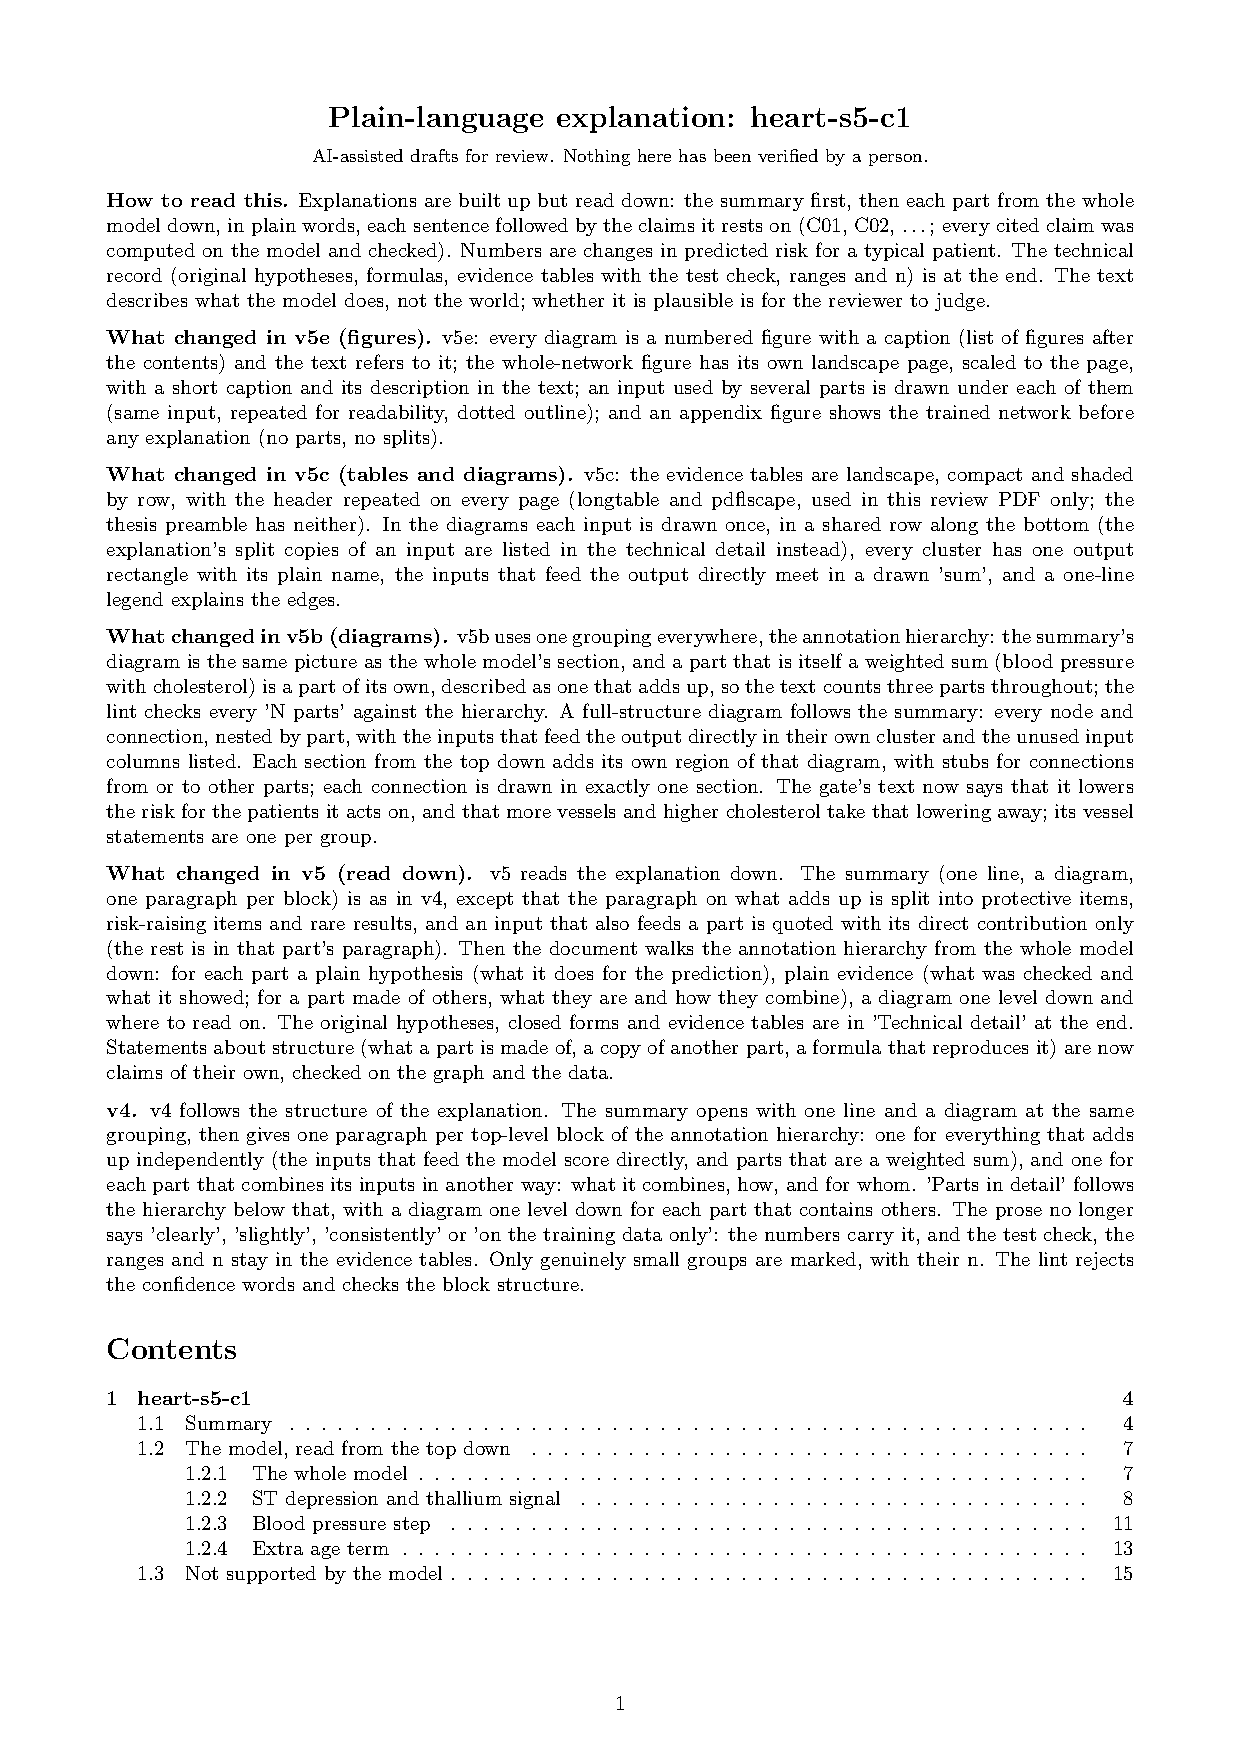
\includepdf[pages={1-5},addtotoc={1,section,1,{heart-s5-c1: plain-language explanation (read-down document)},plain:heart-s5-c1}]{heart-s5-c1/heart-s5-c1-plain-v5.pdf}
\includepdf[pages={6},landscape]{heart-s5-c1/heart-s5-c1-plain-v5.pdf}
\includepdf[pages={7-16}]{heart-s5-c1/heart-s5-c1-plain-v5.pdf}
\includepdf[pages={17-19},landscape]{heart-s5-c1/heart-s5-c1-plain-v5.pdf}
\includepdf[pages={20}]{heart-s5-c1/heart-s5-c1-plain-v5.pdf}
\includepdf[pages={21},landscape]{heart-s5-c1/heart-s5-c1-plain-v5.pdf}
\includepdf[pages={22}]{heart-s5-c1/heart-s5-c1-plain-v5.pdf}
\includepdf[pages={23},landscape]{heart-s5-c1/heart-s5-c1-plain-v5.pdf}
\includepdf[pages={24}]{heart-s5-c1/heart-s5-c1-plain-v5.pdf}
\includepdf[pages={25},landscape]{heart-s5-c1/heart-s5-c1-plain-v5.pdf}
\includepdf[pages={26}]{heart-s5-c1/heart-s5-c1-plain-v5.pdf}
\includepdf[pages={27},landscape]{heart-s5-c1/heart-s5-c1-plain-v5.pdf}
\includepdf[pages={28}]{heart-s5-c1/heart-s5-c1-plain-v5.pdf}
\addcontentsline{toc}{section}{heart-s5-c1: coverage certificate}
% Coverage certificate for heart-s5-c1 (genome 4f9f15fb-446b-4560-9704-c7b1a83617b5); content sha256 f3feba786432f89359505ee8928bcbe868228dc48e57707b5b20ab57f49b46fb.
\providecommand{\explaneatcertdir}[1]{}
\begin{drafted}[heart-s5-c1 coverage certificate]
\section{Coverage certificate: heart-s5-c1}\label{app:heart-s5-c1:sec}
Provenance, coverage and checks of the explanation, rendered from the canonical JSON record \texttt{heart-s5-c1.json} (schema 1.4.0, SHA-256 \texttt{f3feba786432f893}\ldots). The explanation itself (summary, parts, evidence, figures) is the read-down document before this page.

\begin{table}[htbp]
\centering\small
\begin{tabularx}{\linewidth}{@{}lX@{}}
\toprule
Dataset & Heart Disease (binary, prepared) \\
Experiment & 10seed-heart-s5, seed 5 \\
Genome & \texttt{4f9f15fb-446b-4560-9704-c7b1a83617b5} (NEAT key 9259, generation 39) \\
Explanation & \texttt{39c7fe21-518b-4517-8765-7e6008dc7d98} (36 operations) \\
Train AUC / accuracy & 0.9418 / 0.8719 (n = 242) \\
Test AUC / accuracy & 0.8869 / 0.8033 (n = 61) \\
Output activation & sigmoid \\
Phenotype & 30 nodes (26 inputs, 3 hidden, 1 output), 31 enabled edges \\
Explained model state & 36 nodes, 33 enabled edges \\
Refactoring operations & add\_\allowbreak{}identity\_\allowbreak{}node 2, split\_\allowbreak{}node 4 \\
Function preservation & max $|\Delta\,\mathrm{output}|$ = $2.22\times 10^{-16}$ on the training split \\
Annotations & 4 (3 leaf, 1 composition) \\
Structural coverage & 1 (35 of 35 candidate nodes; 4 Null) \\
Compositional coverage & 1 \\
Uncovered nodes / edges & 0 / 0 \\
Missing compositions & 0 \\
Full coverage & yes \\
Drafted by & AI-assisted draft \\
Verified by & unverified \\
Record hash (SHA-256) & \texttt{f3feba786432f893}\ldots \\
\bottomrule
\end{tabularx}
\caption{Explanation certificate summary: heart-s5-c1.}
\label{app:heart-s5-c1:summary}
\end{table}
\subsection{Coverage}\label{app:heart-s5-c1:coverage}
Coverage is computed by the current code (the function behind the \texttt{get\_coverage} tool) under these conventions. \emph{Candidate nodes} are all nodes of the explained model state except the output nodes. A candidate node is \emph{covered} when some annotation of the hierarchy (a leaf, or a composition together with its descendants) contains it and all its enabled outgoing edges. \emph{Exact Null} parts, which have no effect on any output for any input, count as covered: nodes with no path to an output over enabled, non-zero-weight edges (disconnected inputs and dead ends), and edges that have zero weight or touch such a node. Compositional coverage is the fraction of required compositions present: every annotation except a single global root containing every output must have a parent; a parentless, childless annotation made only of Null nodes is exempt.

\begin{itemize}
\item \textbf{Null, disconnected input (4):} \texttt{-11} (fbs:1), \texttt{-13} (restecg:1), \texttt{-14} (restecg:2), \texttt{-3} (sex:1).
\item \textbf{Uncovered nodes:} none.
\item \textbf{Uncovered edges:} none.
\item \textbf{Missing compositions:} none.
\end{itemize}
\noindent\textbf{Agreement with the \texttt{get\_coverage} tool:} yes.

\subsection{Closed-form checks}\label{app:heart-s5-c1:closedform}
{\small\noindent\begin{tabularx}{\linewidth}{@{}lXrr@{}}
\toprule Tag & Annotation & Closed form vs forward pass & Exact function vs forward pass \\ \midrule
A1 & heart\_\allowbreak{}disease\_\allowbreak{}logit & 0.00186 & $2.78\times 10^{-16}$ \\
A2 & ischaemia\_\allowbreak{}gate & 0.0113 & $1.78\times 10^{-15}$ \\
A3 & bp\_\allowbreak{}offset\_\allowbreak{}gate & $8.86\times 10^{-4}$ & $8.88\times 10^{-16}$ \\
A4 & age\_\allowbreak{}gate\_\allowbreak{}without\_\allowbreak{}ischaemia & $4.99\times 10^{-4}$ & $2.22\times 10^{-16}$ \\
\bottomrule
\end{tabularx}\par}
\subsection{Refactoring operations}\label{app:heart-s5-c1:operations}
The explained model state is the phenotype after these operations, replayed in order. All are function-preserving; the largest change in the model output over the 242 training rows is $2.22\times 10^{-16}$ (tolerance $1.00\times 10^{-9}$).
\begin{itemize}
\item \#26: split \texttt{-26} into \texttt{-26\_\allowbreak{}a}, \texttt{-26\_\allowbreak{}b}.
\item \#27: split \texttt{-6} into \texttt{-6\_\allowbreak{}a}, \texttt{-6\_\allowbreak{}b}.
\item \#28: split \texttt{-8} into \texttt{-8\_\allowbreak{}a}, \texttt{-8\_\allowbreak{}b}.
\item \#29: split \texttt{-1} into \texttt{-1\_\allowbreak{}a}, \texttt{-1\_\allowbreak{}b}.
\item \#30: identity node \texttt{identity\_\allowbreak{}290} before \texttt{290} (1 connection(s)).
\item \#31: identity node \texttt{identity\_\allowbreak{}1987} before \texttt{1987} (1 connection(s)).
\end{itemize}
\subsection{Audit against the definitions}\label{app:heart-s5-c1:audit}
Automatic findings on the stored explanation (codes as in the JSON record's \texttt{issues}); they flag what an examiner should check, not verdicts.
\begin{itemize}
\item \textsc{warning} \texttt{unverified}: No human verification is recorded for this explanation.
\end{itemize}
\end{drafted}

\clearpage
\section*{12. heart-s5-c2: verification checklist}
\addcontentsline{toc}{section}{12. heart-s5-c2: verification checklist}
\label{rev:heart-s5-c2}
\textbf{Already recorded:} nothing (no verdict in the record).

\textbf{Recorded vs live.} Agent = the drafting agent's report; orchestrator = the record's automated re-check; live = this export (current code, training split).

{\footnotesize
\begin{tabularx}{\linewidth}{@{}>{\raggedright\arraybackslash}X>{\raggedright\arraybackslash}p{2.1cm}>{\raggedright\arraybackslash}p{3.0cm}>{\raggedright\arraybackslash}p{3.0cm}l@{}}
\toprule
Check & Agent & Orchestrator & Live & Status \\
\midrule
Function preservation, max $|$change in output$|$ & 2.22e-16 & 2.22e-16 & 2.22e-16 & agree \\
Closed-form max abs error (all leaves) & 0.0173 & 0.0173 & 0.0173 & agree \\
Numeric-function max abs error & n/a & 1.78e-15 & 1.78e-15 & agree \\
Structural coverage & 1 & 1 & 1 & agree \\
Compositional coverage & 1 & 1 & 1 & agree \\
Hierarchy complete & yes & yes & yes & agree \\
Root annotation & n/a & heart\_\allowbreak{}disease\_\allowbreak{}logit & heart\_\allowbreak{}disease\_\allowbreak{}logit & agree \\
Leaf / composition counts & 5 / 1 & n/a & 5 / 1 & agree \\
Operation counts & 5 splits, 2 identity & add identity node 2, annotate 6, rename node 26, split node 5 & add identity node 2, annotate 6, rename node 26, split node 5 & agree \\
Full coverage & yes & yes & yes & agree \\
\bottomrule
\end{tabularx}}

\textbf{What to look at.}
\begin{itemize}
\item Largest closed-form error: \texttt{ischaemia\_\allowbreak{}gate} (0.0173). This is the cost of the 3 s.f. display rounding, in the exit's own units; the numeric function is exact. Check that the rounded formula still supports the hypothesis as worded.
\item Strong claim in \texttt{lvh\_\allowbreak{}without\_\allowbreak{}exercise\_\allowbreak{}angina}: \emph{``Hypothesis: a binary AND: open (constant 0.324, +0.236 logit) only for patients with left ventricular hypertrophy on the resting ECG and no exercise-induced angina, zero otherwise.''} Is this (exactness, threshold, rare category) supported by the evidence, or fitted to a few rows?
\item Strong claim in \texttt{high\_\allowbreak{}fasting\_\allowbreak{}sugar}: \emph{``Hypothesis: a small additive term for high fasting sugar (exactly linear on the two values of fbs:1);''} Is this (exactness, threshold, rare category) supported by the evidence, or fitted to a few rows?
\item 5 split(s), all of input nodes (an input feeding two annotations). These are routine; check only that each input copy sits in the annotation whose hypothesis uses it.
\item Read the root's hypothesis against its closed form: does the stated combination of children (additive, gated, serial) match the formula?
\end{itemize}
\textbf{Tool notes (record):} get\_\allowbreak{}input\_\allowbreak{}distribution does not accept sample\_\allowbreak{}fraction (called with max\_\allowbreak{}samples only; all 242 rows used). get\_\allowbreak{}viz\_\allowbreak{}summary requires viz\_\allowbreak{}type (sensitivity used). compute\_\allowbreak{}shap (kernel, all 242 train rows) gives the five unconnected inputs mean $|$SHAP$|$ about 0.001 instead of exactly 0 (sampling noise). get\_\allowbreak{}model\_\allowbreak{}state's 'operations' key is absent, so op counts come from check\_\allowbreak{}explanation.py. The agent sandbox refused compound shell commands, so tools were called through a small Python subprocess wrapper in scratch (same xn.py).

\textbf{Plain-language layer} (AI-assisted draft for review (unverified)): the read-down document follows this page (summary, parts, evidence, worth checking; also \texttt{heart-s5-c2-plain-v5.pdf} in this genome's folder). Record a verdict on it with \texttt{uv run python -m explaneat export record-plain-verdict heart-s5-c2 --verified --minutes N --notes "..."}.

\textbf{Verdict.}

\begin{tabularx}{\linewidth}{@{}lX@{}}
Verified (correct as it stands, or after my changes): & $\square$ yes \quad $\square$ no \\[4pt]
Minutes: & \rule{3cm}{0.4pt} \\[4pt]
Changes: & \rule{\linewidth}{0.4pt} \\[10pt]
 & \rule{\linewidth}{0.4pt} \\[4pt]
Notes: & \rule{\linewidth}{0.4pt} \\[10pt]
 & \rule{\linewidth}{0.4pt} \\
\end{tabularx}

\textbf{Record it} (writes \texttt{mike\_verification} into \texttt{experiments/10seed/explanations/heart-s5-c2.json}; use \texttt{-{}-not-verified} for no; rebuild the CSVs with \texttt{uv run python experiments/10seed/build\_explanations\_csv.py}):

{\footnotesize\raggedright\texttt{uv run python -m explaneat export record-verdict heart-s5-c2 --verified --minutes N --changes "..." --notes "..."}\par}


\clearpage
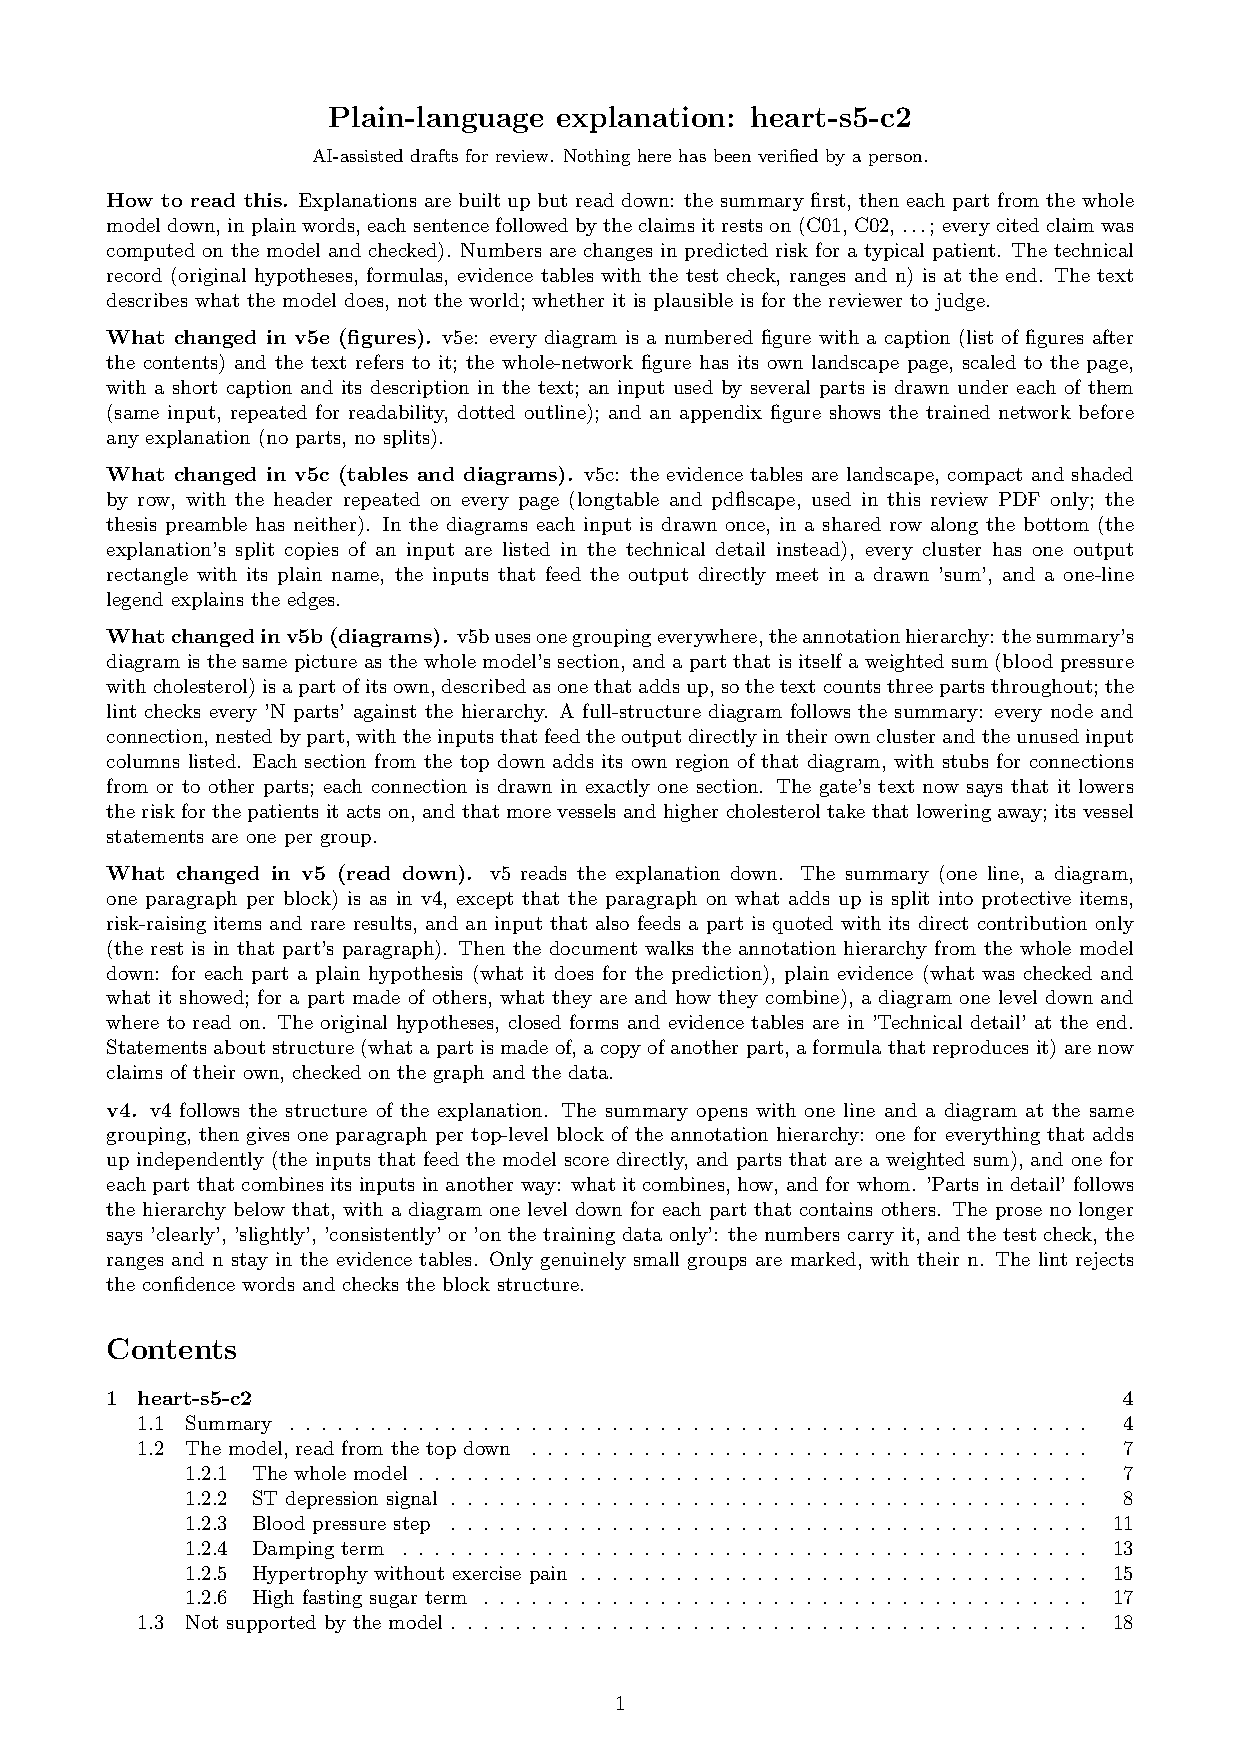
\includepdf[pages={1-5},addtotoc={1,section,1,{heart-s5-c2: plain-language explanation (read-down document)},plain:heart-s5-c2}]{heart-s5-c2/heart-s5-c2-plain-v5.pdf}
\includepdf[pages={6},landscape]{heart-s5-c2/heart-s5-c2-plain-v5.pdf}
\includepdf[pages={7-19}]{heart-s5-c2/heart-s5-c2-plain-v5.pdf}
\includepdf[pages={20-22},landscape]{heart-s5-c2/heart-s5-c2-plain-v5.pdf}
\includepdf[pages={23}]{heart-s5-c2/heart-s5-c2-plain-v5.pdf}
\includepdf[pages={24},landscape]{heart-s5-c2/heart-s5-c2-plain-v5.pdf}
\includepdf[pages={25}]{heart-s5-c2/heart-s5-c2-plain-v5.pdf}
\includepdf[pages={26},landscape]{heart-s5-c2/heart-s5-c2-plain-v5.pdf}
\includepdf[pages={27}]{heart-s5-c2/heart-s5-c2-plain-v5.pdf}
\includepdf[pages={28},landscape]{heart-s5-c2/heart-s5-c2-plain-v5.pdf}
\includepdf[pages={29}]{heart-s5-c2/heart-s5-c2-plain-v5.pdf}
\includepdf[pages={30},landscape]{heart-s5-c2/heart-s5-c2-plain-v5.pdf}
\includepdf[pages={31}]{heart-s5-c2/heart-s5-c2-plain-v5.pdf}
\includepdf[pages={32},landscape]{heart-s5-c2/heart-s5-c2-plain-v5.pdf}
\includepdf[pages={33}]{heart-s5-c2/heart-s5-c2-plain-v5.pdf}
\includepdf[pages={34},landscape]{heart-s5-c2/heart-s5-c2-plain-v5.pdf}
\includepdf[pages={35}]{heart-s5-c2/heart-s5-c2-plain-v5.pdf}
\addcontentsline{toc}{section}{heart-s5-c2: coverage certificate}
% Coverage certificate for heart-s5-c2 (genome 57c311c6-56f5-4c5d-a475-46433ef58bf2); content sha256 e5293773fce87faec815a166111f195edf55b68bde14ba046b51556ab442dcea.
\providecommand{\explaneatcertdir}[1]{}
\begin{drafted}[heart-s5-c2 coverage certificate]
\section{Coverage certificate: heart-s5-c2}\label{app:heart-s5-c2:sec}
Provenance, coverage and checks of the explanation, rendered from the canonical JSON record \texttt{heart-s5-c2.json} (schema 1.4.0, SHA-256 \texttt{e5293773fce87fae}\ldots). The explanation itself (summary, parts, evidence, figures) is the read-down document before this page.

\begin{table}[htbp]
\centering\small
\begin{tabularx}{\linewidth}{@{}lX@{}}
\toprule
Dataset & Heart Disease (binary, prepared) \\
Experiment & 10seed-heart-s5, seed 5 \\
Genome & \texttt{57c311c6-56f5-4c5d-a475-46433ef58bf2} (NEAT key 9858, generation 39) \\
Explanation & \texttt{dabdb4bb-e227-46eb-a995-d4123373f234} (39 operations) \\
Train AUC / accuracy & 0.9389 / 0.8802 (n = 242) \\
Test AUC / accuracy & 0.8922 / 0.8197 (n = 61) \\
Output activation & sigmoid \\
Phenotype & 32 nodes (26 inputs, 5 hidden, 1 output), 35 enabled edges \\
Explained model state & 41 nodes, 37 enabled edges \\
Refactoring operations & add\_\allowbreak{}identity\_\allowbreak{}node 2, split\_\allowbreak{}node 5 \\
Function preservation & max $|\Delta\,\mathrm{output}|$ = $2.22\times 10^{-16}$ on the training split \\
Annotations & 6 (5 leaf, 1 composition) \\
Structural coverage & 1 (40 of 40 candidate nodes; 5 Null) \\
Compositional coverage & 1 \\
Uncovered nodes / edges & 0 / 0 \\
Missing compositions & 0 \\
Full coverage & yes \\
Drafted by & AI-assisted draft \\
Verified by & unverified \\
Record hash (SHA-256) & \texttt{e5293773fce87fae}\ldots \\
\bottomrule
\end{tabularx}
\caption{Explanation certificate summary: heart-s5-c2.}
\label{app:heart-s5-c2:summary}
\end{table}
\subsection{Coverage}\label{app:heart-s5-c2:coverage}
Coverage is computed by the current code (the function behind the \texttt{get\_coverage} tool) under these conventions. \emph{Candidate nodes} are all nodes of the explained model state except the output nodes. A candidate node is \emph{covered} when some annotation of the hierarchy (a leaf, or a composition together with its descendants) contains it and all its enabled outgoing edges. \emph{Exact Null} parts, which have no effect on any output for any input, count as covered: nodes with no path to an output over enabled, non-zero-weight edges (disconnected inputs and dead ends), and edges that have zero weight or touch such a node. Compositional coverage is the fraction of required compositions present: every annotation except a single global root containing every output must have a parent; a parentless, childless annotation made only of Null nodes is exempt.

\begin{itemize}
\item \textbf{Null, disconnected input (5):} \texttt{-13} (restecg:1), \texttt{-20} (slope:2), \texttt{-26} (thal:7), \texttt{-3} (sex:1), \texttt{-5} (cp:2).
\item \textbf{Uncovered nodes:} none.
\item \textbf{Uncovered edges:} none.
\item \textbf{Missing compositions:} none.
\end{itemize}
\noindent\textbf{Agreement with the \texttt{get\_coverage} tool:} yes.

\subsection{Closed-form checks}\label{app:heart-s5-c2:closedform}
{\small\noindent\begin{tabularx}{\linewidth}{@{}lXrr@{}}
\toprule Tag & Annotation & Closed form vs forward pass & Exact function vs forward pass \\ \midrule
A1 & heart\_\allowbreak{}disease\_\allowbreak{}logit & 0.00243 & $2.22\times 10^{-16}$ \\
A2 & ischaemia\_\allowbreak{}gate & 0.0173 & 0 \\
A3 & bp\_\allowbreak{}offset\_\allowbreak{}gate & 0.00119 & $1.78\times 10^{-15}$ \\
A4 & ischaemia\_\allowbreak{}damping\_\allowbreak{}thal6 & 0.00134 & $2.22\times 10^{-16}$ \\
A5 & lvh\_\allowbreak{}without\_\allowbreak{}exercise\_\allowbreak{}angina & $2.52\times 10^{-4}$ & 0 \\
A6 & high\_\allowbreak{}fasting\_\allowbreak{}sugar & $3.12\times 10^{-4}$ & 0 \\
\bottomrule
\end{tabularx}\par}
\subsection{Refactoring operations}\label{app:heart-s5-c2:operations}
The explained model state is the phenotype after these operations, replayed in order. All are function-preserving; the largest change in the model output over the 242 training rows is $2.22\times 10^{-16}$ (tolerance $1.00\times 10^{-9}$).
\begin{itemize}
\item \#26: split \texttt{-12} into \texttt{-12\_\allowbreak{}a}, \texttt{-12\_\allowbreak{}b}.
\item \#27: split \texttt{-17} into \texttt{-17\_\allowbreak{}a}, \texttt{-17\_\allowbreak{}b}, \texttt{-17\_\allowbreak{}c}.
\item \#28: split \texttt{-25} into \texttt{-25\_\allowbreak{}a}, \texttt{-25\_\allowbreak{}b}, \texttt{-25\_\allowbreak{}c}.
\item \#29: split \texttt{-8} into \texttt{-8\_\allowbreak{}a}, \texttt{-8\_\allowbreak{}b}.
\item \#30: split \texttt{-6} into \texttt{-6\_\allowbreak{}a}, \texttt{-6\_\allowbreak{}b}.
\item \#31: identity node \texttt{identity\_\allowbreak{}290} before \texttt{290} (1 connection(s)).
\item \#32: identity node \texttt{identity\_\allowbreak{}1416} before \texttt{1416} (1 connection(s)).
\end{itemize}
\subsection{Audit against the definitions}\label{app:heart-s5-c2:audit}
Automatic findings on the stored explanation (codes as in the JSON record's \texttt{issues}); they flag what an examiner should check, not verdicts.
\begin{itemize}
\item \textsc{warning} \texttt{unverified}: No human verification is recorded for this explanation.
\end{itemize}
\end{drafted}

\clearpage
\section*{13. heart-s5-c3: verification checklist}
\addcontentsline{toc}{section}{13. heart-s5-c3: verification checklist}
\label{rev:heart-s5-c3}
\textbf{Already recorded:} nothing (no verdict in the record).

\textbf{Recorded vs live.} Agent = the drafting agent's report; orchestrator = the record's automated re-check; live = this export (current code, training split).

{\footnotesize
\begin{tabularx}{\linewidth}{@{}>{\raggedright\arraybackslash}X>{\raggedright\arraybackslash}p{2.1cm}>{\raggedright\arraybackslash}p{3.0cm}>{\raggedright\arraybackslash}p{3.0cm}l@{}}
\toprule
Check & Agent & Orchestrator & Live & Status \\
\midrule
Function preservation, max $|$change in output$|$ & 2.22e-16 & 2.22e-16 & 2.22e-16 & agree \\
Closed-form max abs error (all leaves) & 0.0205 & 0.0205 & 0.0205 & agree \\
Numeric-function max abs error & n/a & 1.78e-15 & 1.78e-15 & agree \\
Structural coverage & 1 & 1 & 1 & agree \\
Compositional coverage & 1 & 1 & 1 & agree \\
Hierarchy complete & yes & yes & yes & agree \\
Root annotation & n/a & heart\_\allowbreak{}disease\_\allowbreak{}logit & heart\_\allowbreak{}disease\_\allowbreak{}logit & agree \\
Leaf / composition counts & 2 / 1 & n/a & 2 / 1 & agree \\
Operation counts & 1 splits, 0 identity & annotate 3, rename node 26, split node 1 & annotate 3, rename node 26, split node 1 & agree \\
Full coverage & yes & yes & yes & agree \\
\bottomrule
\end{tabularx}}

\textbf{What to look at.}
\begin{itemize}
\item Largest closed-form error: \texttt{ischaemia\_\allowbreak{}chain} (0.0205). This is the cost of the 3 s.f. display rounding, in the exit's own units; the numeric function is exact. Check that the rounded formula still supports the hypothesis as worded.
\item 1 split(s), all of input nodes (an input feeding two annotations). These are routine; check only that each input copy sits in the annotation whose hypothesis uses it.
\item Read the root's hypothesis against its closed form: does the stated combination of children (additive, gated, serial) match the formula?
\end{itemize}
\textbf{Tool notes (record):} get\_\allowbreak{}input\_\allowbreak{}distribution does not accept sample\_\allowbreak{}fraction (called with max\_\allowbreak{}samples only; all 242 rows used). get\_\allowbreak{}viz\_\allowbreak{}summary requires viz\_\allowbreak{}type (sensitivity and line\_\allowbreak{}plot used). add\_\allowbreak{}identity\_\allowbreak{}node cannot intercept a node's only input (by design), which forced the two-exit leaf. compute\_\allowbreak{}shap (kernel, all 242 train rows) gives the seven unconnected inputs mean $|$SHAP$|$ about 0.001 instead of exactly 0 (sampling noise). The agent sandbox refused compound shell commands, so tools were called through a small Python subprocess wrapper in scratch (same species\_\allowbreak{}leads/\allowbreak{}xn.py)\allowbreak{}.

\textbf{Plain-language layer} (AI-assisted draft for review (unverified)): the read-down document follows this page (summary, parts, evidence, worth checking; also \texttt{heart-s5-c3-plain-v5.pdf} in this genome's folder). Record a verdict on it with \texttt{uv run python -m explaneat export record-plain-verdict heart-s5-c3 --verified --minutes N --notes "..."}.

\textbf{Verdict.}

\begin{tabularx}{\linewidth}{@{}lX@{}}
Verified (correct as it stands, or after my changes): & $\square$ yes \quad $\square$ no \\[4pt]
Minutes: & \rule{3cm}{0.4pt} \\[4pt]
Changes: & \rule{\linewidth}{0.4pt} \\[10pt]
 & \rule{\linewidth}{0.4pt} \\[4pt]
Notes: & \rule{\linewidth}{0.4pt} \\[10pt]
 & \rule{\linewidth}{0.4pt} \\
\end{tabularx}

\textbf{Record it} (writes \texttt{mike\_verification} into \texttt{experiments/10seed/explanations/heart-s5-c3.json}; use \texttt{-{}-not-verified} for no; rebuild the CSVs with \texttt{uv run python experiments/10seed/build\_explanations\_csv.py}):

{\footnotesize\raggedright\texttt{uv run python -m explaneat export record-verdict heart-s5-c3 --verified --minutes N --changes "..." --notes "..."}\par}


\clearpage
\includepdf[pages={1-4},addtotoc={1,section,1,{heart-s5-c3: plain-language explanation (read-down document)},plain:heart-s5-c3}]{heart-s5-c3/heart-s5-c3-plain-v5.pdf}
\includepdf[pages={5},landscape]{heart-s5-c3/heart-s5-c3-plain-v5.pdf}
\includepdf[pages={6-14}]{heart-s5-c3/heart-s5-c3-plain-v5.pdf}
\includepdf[pages={15-16},landscape]{heart-s5-c3/heart-s5-c3-plain-v5.pdf}
\includepdf[pages={17}]{heart-s5-c3/heart-s5-c3-plain-v5.pdf}
\includepdf[pages={18},landscape]{heart-s5-c3/heart-s5-c3-plain-v5.pdf}
\includepdf[pages={19}]{heart-s5-c3/heart-s5-c3-plain-v5.pdf}
\includepdf[pages={20},landscape]{heart-s5-c3/heart-s5-c3-plain-v5.pdf}
\includepdf[pages={21}]{heart-s5-c3/heart-s5-c3-plain-v5.pdf}
\includepdf[pages={22},landscape]{heart-s5-c3/heart-s5-c3-plain-v5.pdf}
\includepdf[pages={23}]{heart-s5-c3/heart-s5-c3-plain-v5.pdf}
\addcontentsline{toc}{section}{heart-s5-c3: coverage certificate}
% Coverage certificate for heart-s5-c3 (genome 96fb45fb-972d-4aaa-b6d5-01fc63fbc4e6); content sha256 644db15ecc0191f8ed73b9a23757dccfcf5f1809df487f9171d22800751515e6.
\providecommand{\explaneatcertdir}[1]{}
\begin{drafted}[heart-s5-c3 coverage certificate]
\section{Coverage certificate: heart-s5-c3}\label{app:heart-s5-c3:sec}
Provenance, coverage and checks of the explanation, rendered from the canonical JSON record \texttt{heart-s5-c3.json} (schema 1.4.0, SHA-256 \texttt{644db15ecc0191f8}\ldots). The explanation itself (summary, parts, evidence, figures) is the read-down document before this page.

\begin{table}[htbp]
\centering\small
\begin{tabularx}{\linewidth}{@{}lX@{}}
\toprule
Dataset & Heart Disease (binary, prepared) \\
Experiment & 10seed-heart-s5, seed 5 \\
Genome & \texttt{96fb45fb-972d-4aaa-b6d5-01fc63fbc4e6} (NEAT key 9698, generation 39) \\
Explanation & \texttt{1b3f669d-9fb5-4126-b6e4-35535db7b3b1} (30 operations) \\
Train AUC / accuracy & 0.9376 / 0.8884 (n = 242) \\
Test AUC / accuracy & 0.9084 / 0.8197 (n = 61) \\
Output activation & sigmoid \\
Phenotype & 31 nodes (26 inputs, 4 hidden, 1 output), 26 enabled edges \\
Explained model state & 32 nodes, 26 enabled edges \\
Refactoring operations & split\_\allowbreak{}node 1 \\
Function preservation & max $|\Delta\,\mathrm{output}|$ = $2.22\times 10^{-16}$ on the training split \\
Annotations & 3 (2 leaf, 1 composition) \\
Structural coverage & 1 (31 of 31 candidate nodes; 7 Null) \\
Compositional coverage & 1 \\
Uncovered nodes / edges & 0 / 0 \\
Missing compositions & 0 \\
Full coverage & yes \\
Drafted by & AI-assisted draft \\
Verified by & unverified \\
Record hash (SHA-256) & \texttt{644db15ecc0191f8}\ldots \\
\bottomrule
\end{tabularx}
\caption{Explanation certificate summary: heart-s5-c3.}
\label{app:heart-s5-c3:summary}
\end{table}
\subsection{Coverage}\label{app:heart-s5-c3:coverage}
Coverage is computed by the current code (the function behind the \texttt{get\_coverage} tool) under these conventions. \emph{Candidate nodes} are all nodes of the explained model state except the output nodes. A candidate node is \emph{covered} when some annotation of the hierarchy (a leaf, or a composition together with its descendants) contains it and all its enabled outgoing edges. \emph{Exact Null} parts, which have no effect on any output for any input, count as covered: nodes with no path to an output over enabled, non-zero-weight edges (disconnected inputs and dead ends), and edges that have zero weight or touch such a node. Compositional coverage is the fraction of required compositions present: every annotation except a single global root containing every output must have a parent; a parentless, childless annotation made only of Null nodes is exempt.

\begin{itemize}
\item \textbf{Null, disconnected input (7):} \texttt{-11} (fbs:1), \texttt{-13} (restecg:1), \texttt{-14} (restecg:2), \texttt{-16} (exang:0), \texttt{-20} (slope:2), \texttt{-3} (sex:1), \texttt{-5} (cp:2).
\item \textbf{Uncovered nodes:} none.
\item \textbf{Uncovered edges:} none.
\item \textbf{Missing compositions:} none.
\end{itemize}
\noindent\textbf{Agreement with the \texttt{get\_coverage} tool:} yes.

\subsection{Closed-form checks}\label{app:heart-s5-c3:closedform}
{\small\noindent\begin{tabularx}{\linewidth}{@{}lXrr@{}}
\toprule Tag & Annotation & Closed form vs forward pass & Exact function vs forward pass \\ \midrule
A1 & heart\_\allowbreak{}disease\_\allowbreak{}logit & 0.00216 & $2.78\times 10^{-16}$ \\
A2 & ischaemia\_\allowbreak{}chain & 0.0205 & $1.78\times 10^{-15}$ \\
A3 & age\_\allowbreak{}hinge & $2.75\times 10^{-4}$ & 0 \\
\bottomrule
\end{tabularx}\par}
\subsection{Refactoring operations}\label{app:heart-s5-c3:operations}
The explained model state is the phenotype after these operations, replayed in order. All are function-preserving; the largest change in the model output over the 242 training rows is $2.22\times 10^{-16}$ (tolerance $1.00\times 10^{-9}$).
\begin{itemize}
\item \#26: split \texttt{-12} into \texttt{-12\_\allowbreak{}a}, \texttt{-12\_\allowbreak{}b}.
\end{itemize}
\subsection{Audit against the definitions}\label{app:heart-s5-c3:audit}
Automatic findings on the stored explanation (codes as in the JSON record's \texttt{issues}); they flag what an examiner should check, not verdicts.
\begin{itemize}
\item \textsc{warning} \texttt{unverified}: No human verification is recorded for this explanation.
\end{itemize}
\end{drafted}

\clearpage
\end{document}
